%%
%% This is file `sample-manuscript.tex',
%% generated with the docstrip utility.
%%
%% The original source files were:
%%
%% samples.dtx  (with options: `all,proceedings,bibtex,manuscript')
%% 
%% IMPORTANT NOTICE:
%% 
%% For the copyright see the source file.
%% 
%% Any modified versions of this file must be renamed
%% with new filenames distinct from sample-manuscript.tex.
%% 
%% For distribution of the original source see the terms
%% for copying and modification in the file samples.dtx.
%% 
%% This generated file may be distributed as long as the
%% original source files, as listed above, are part of the
%% same distribution. (The sources need not necessarily be
%% in the same archive or directory.)
%%
%%
%% Commands for TeXCount
%TC:macro \cite [option:text,text]
%TC:macro \citep [option:text,text]
%TC:macro \citet [option:text,text]
%TC:envir table 0 1
%TC:envir table* 0 1
%TC:envir tabular [ignore] word
%TC:envir displaymath 0 word
%TC:envir math 0 word
%TC:envir comment 0 0
%%
%% The first command in your LaTeX source must be the \documentclass
%% command.
%%
%% For submission and review of your manuscript please change the
%% command to \documentclass[manuscript, screen, review]{acmart}.
%%
%% When submitting camera ready or to TAPS, please change the command
%% to \documentclass[sigconf]{acmart} or whichever template is required
%% for your publication.
%%
%%
% \documentclass[manuscript,screen,review]{acmart}
% \documentclass[manuscript,screen,review,anonymous]{acmart}
\documentclass[sigconf]{acmart}
%%
%% \BibTeX command to typeset BibTeX logo in the docs
\AtBeginDocument{%
  \providecommand\BibTeX{{%
    Bib\TeX}}}

%% Rights management information.  This information is sent to you
%% when you complete the rights form.  These commands have SAMPLE
%% values in them; it is your responsibility as an author to replace
%% the commands and values with those provided to you when you
%% complete the rights form.
\setcopyright{acmlicensed}
\copyrightyear{2018}
\acmYear{2018}
\acmDOI{XXXXXXX.XXXXXXX}
%% These commands are for a PROCEEDINGS abstract or paper.
\acmConference[FAccT '25]{ACM Conference on Fairness, Accountability, and Transparency}{June 03--05, 2025}{Athens, Greece}
%%
%%  Uncomment \acmBooktitle if the title of the proceedings is different
%%  from ``Proceedings of ...''!
%%
%%\acmBooktitle{Woodstock '18: ACM Symposium on Neural Gaze Detection,
%%  June 03--05, 2018, Woodstock, NY}
\acmISBN{978-1-4503-XXXX-X/2018/06}


%%
%% Submission ID.
%% Use this when submitting an article to a sponsored event. You'll
%% receive a unique submission ID from the organizers
%% of the event, and this ID should be used as the parameter to this command.
%%\acmSubmissionID{123-A56-BU3}

%%
%% For managing citations, it is recommended to use bibliography
%% files in BibTeX format.
%%
%% You can then either use BibTeX with the ACM-Reference-Format style,
%% or BibLaTeX with the acmnumeric or acmauthoryear sytles, that include
%% support for advanced citation of software artefact from the
%% biblatex-software package, also separately available on CTAN.
%%
%% Look at the sample-*-biblatex.tex files for templates showcasing
%% the biblatex styles.
%%

%%
%% The majority of ACM publications use numbered citations and
%% references.  The command \citestyle{authoryear} switches to the
%% "author year" style.
%%
%% If you are preparing content for an event
%% sponsored by ACM SIGGRAPH, you must use the "author year" style of
%% citations and references.
%% Uncommenting
%% the next command will enable that style.
%%\citestyle{acmauthoryear}

\usepackage{natbib}
\renewcommand{\bibname}{References}
\renewcommand{\bibsection}{\subsubsection*{\bibname}}

% If you use BibTeX in apalike style, activate the following line:
% \bibliographystyle{apalike}

% Optional math commands from https://github.com/goodfeli/dlbook_notation.
%%%%% NEW MATH DEFINITIONS %%%%%

\usepackage{amsmath,amsfonts,bm}

% Mark sections of captions for referring to divisions of figures
\newcommand{\figleft}{{\em (Left)}}
\newcommand{\figcenter}{{\em (Center)}}
\newcommand{\figright}{{\em (Right)}}
\newcommand{\figtop}{{\em (Top)}}
\newcommand{\figbottom}{{\em (Bottom)}}
\newcommand{\captiona}{{\em (a)}}
\newcommand{\captionb}{{\em (b)}}
\newcommand{\captionc}{{\em (c)}}
\newcommand{\captiond}{{\em (d)}}

% Highlight a newly defined term
\newcommand{\newterm}[1]{{\bf #1}}


% Figure reference, lower-case.
\def\figref#1{figure~\ref{#1}}
% Figure reference, capital. For start of sentence
\def\Figref#1{Figure~\ref{#1}}
\def\twofigref#1#2{figures \ref{#1} and \ref{#2}}
\def\quadfigref#1#2#3#4{figures \ref{#1}, \ref{#2}, \ref{#3} and \ref{#4}}
% Section reference, lower-case.
\def\secref#1{section~\ref{#1}}
% Section reference, capital.
\def\Secref#1{Section~\ref{#1}}
% Reference to two sections.
\def\twosecrefs#1#2{sections \ref{#1} and \ref{#2}}
% Reference to three sections.
\def\secrefs#1#2#3{sections \ref{#1}, \ref{#2} and \ref{#3}}
% Reference to an equation, lower-case.
\def\eqref#1{equation~\ref{#1}}
% Reference to an equation, upper case
\def\Eqref#1{Equation~\ref{#1}}
% A raw reference to an equation---avoid using if possible
\def\plaineqref#1{\ref{#1}}
% Reference to a chapter, lower-case.
\def\chapref#1{chapter~\ref{#1}}
% Reference to an equation, upper case.
\def\Chapref#1{Chapter~\ref{#1}}
% Reference to a range of chapters
\def\rangechapref#1#2{chapters\ref{#1}--\ref{#2}}
% Reference to an algorithm, lower-case.
\def\algref#1{algorithm~\ref{#1}}
% Reference to an algorithm, upper case.
\def\Algref#1{Algorithm~\ref{#1}}
\def\twoalgref#1#2{algorithms \ref{#1} and \ref{#2}}
\def\Twoalgref#1#2{Algorithms \ref{#1} and \ref{#2}}
% Reference to a part, lower case
\def\partref#1{part~\ref{#1}}
% Reference to a part, upper case
\def\Partref#1{Part~\ref{#1}}
\def\twopartref#1#2{parts \ref{#1} and \ref{#2}}

\def\ceil#1{\lceil #1 \rceil}
\def\floor#1{\lfloor #1 \rfloor}
\def\1{\bm{1}}
\newcommand{\train}{\mathcal{D}}
\newcommand{\valid}{\mathcal{D_{\mathrm{valid}}}}
\newcommand{\test}{\mathcal{D_{\mathrm{test}}}}

\def\eps{{\epsilon}}


% Random variables
\def\reta{{\textnormal{$\eta$}}}
\def\ra{{\textnormal{a}}}
\def\rb{{\textnormal{b}}}
\def\rc{{\textnormal{c}}}
\def\rd{{\textnormal{d}}}
\def\re{{\textnormal{e}}}
\def\rf{{\textnormal{f}}}
\def\rg{{\textnormal{g}}}
\def\rh{{\textnormal{h}}}
\def\ri{{\textnormal{i}}}
\def\rj{{\textnormal{j}}}
\def\rk{{\textnormal{k}}}
\def\rl{{\textnormal{l}}}
% rm is already a command, just don't name any random variables m
\def\rn{{\textnormal{n}}}
\def\ro{{\textnormal{o}}}
\def\rp{{\textnormal{p}}}
\def\rq{{\textnormal{q}}}
\def\rr{{\textnormal{r}}}
\def\rs{{\textnormal{s}}}
\def\rt{{\textnormal{t}}}
\def\ru{{\textnormal{u}}}
\def\rv{{\textnormal{v}}}
\def\rw{{\textnormal{w}}}
\def\rx{{\textnormal{x}}}
\def\ry{{\textnormal{y}}}
\def\rz{{\textnormal{z}}}

% Random vectors
\def\rvepsilon{{\mathbf{\epsilon}}}
\def\rvtheta{{\mathbf{\theta}}}
\def\rva{{\mathbf{a}}}
\def\rvb{{\mathbf{b}}}
\def\rvc{{\mathbf{c}}}
\def\rvd{{\mathbf{d}}}
\def\rve{{\mathbf{e}}}
\def\rvf{{\mathbf{f}}}
\def\rvg{{\mathbf{g}}}
\def\rvh{{\mathbf{h}}}
\def\rvu{{\mathbf{i}}}
\def\rvj{{\mathbf{j}}}
\def\rvk{{\mathbf{k}}}
\def\rvl{{\mathbf{l}}}
\def\rvm{{\mathbf{m}}}
\def\rvn{{\mathbf{n}}}
\def\rvo{{\mathbf{o}}}
\def\rvp{{\mathbf{p}}}
\def\rvq{{\mathbf{q}}}
\def\rvr{{\mathbf{r}}}
\def\rvs{{\mathbf{s}}}
\def\rvt{{\mathbf{t}}}
\def\rvu{{\mathbf{u}}}
\def\rvv{{\mathbf{v}}}
\def\rvw{{\mathbf{w}}}
\def\rvx{{\mathbf{x}}}
\def\rvy{{\mathbf{y}}}
\def\rvz{{\mathbf{z}}}

% Elements of random vectors
\def\erva{{\textnormal{a}}}
\def\ervb{{\textnormal{b}}}
\def\ervc{{\textnormal{c}}}
\def\ervd{{\textnormal{d}}}
\def\erve{{\textnormal{e}}}
\def\ervf{{\textnormal{f}}}
\def\ervg{{\textnormal{g}}}
\def\ervh{{\textnormal{h}}}
\def\ervi{{\textnormal{i}}}
\def\ervj{{\textnormal{j}}}
\def\ervk{{\textnormal{k}}}
\def\ervl{{\textnormal{l}}}
\def\ervm{{\textnormal{m}}}
\def\ervn{{\textnormal{n}}}
\def\ervo{{\textnormal{o}}}
\def\ervp{{\textnormal{p}}}
\def\ervq{{\textnormal{q}}}
\def\ervr{{\textnormal{r}}}
\def\ervs{{\textnormal{s}}}
\def\ervt{{\textnormal{t}}}
\def\ervu{{\textnormal{u}}}
\def\ervv{{\textnormal{v}}}
\def\ervw{{\textnormal{w}}}
\def\ervx{{\textnormal{x}}}
\def\ervy{{\textnormal{y}}}
\def\ervz{{\textnormal{z}}}

% Random matrices
\def\rmA{{\mathbf{A}}}
\def\rmB{{\mathbf{B}}}
\def\rmC{{\mathbf{C}}}
\def\rmD{{\mathbf{D}}}
\def\rmE{{\mathbf{E}}}
\def\rmF{{\mathbf{F}}}
\def\rmG{{\mathbf{G}}}
\def\rmH{{\mathbf{H}}}
\def\rmI{{\mathbf{I}}}
\def\rmJ{{\mathbf{J}}}
\def\rmK{{\mathbf{K}}}
\def\rmL{{\mathbf{L}}}
\def\rmM{{\mathbf{M}}}
\def\rmN{{\mathbf{N}}}
\def\rmO{{\mathbf{O}}}
\def\rmP{{\mathbf{P}}}
\def\rmQ{{\mathbf{Q}}}
\def\rmR{{\mathbf{R}}}
\def\rmS{{\mathbf{S}}}
\def\rmT{{\mathbf{T}}}
\def\rmU{{\mathbf{U}}}
\def\rmV{{\mathbf{V}}}
\def\rmW{{\mathbf{W}}}
\def\rmX{{\mathbf{X}}}
\def\rmY{{\mathbf{Y}}}
\def\rmZ{{\mathbf{Z}}}

% Elements of random matrices
\def\ermA{{\textnormal{A}}}
\def\ermB{{\textnormal{B}}}
\def\ermC{{\textnormal{C}}}
\def\ermD{{\textnormal{D}}}
\def\ermE{{\textnormal{E}}}
\def\ermF{{\textnormal{F}}}
\def\ermG{{\textnormal{G}}}
\def\ermH{{\textnormal{H}}}
\def\ermI{{\textnormal{I}}}
\def\ermJ{{\textnormal{J}}}
\def\ermK{{\textnormal{K}}}
\def\ermL{{\textnormal{L}}}
\def\ermM{{\textnormal{M}}}
\def\ermN{{\textnormal{N}}}
\def\ermO{{\textnormal{O}}}
\def\ermP{{\textnormal{P}}}
\def\ermQ{{\textnormal{Q}}}
\def\ermR{{\textnormal{R}}}
\def\ermS{{\textnormal{S}}}
\def\ermT{{\textnormal{T}}}
\def\ermU{{\textnormal{U}}}
\def\ermV{{\textnormal{V}}}
\def\ermW{{\textnormal{W}}}
\def\ermX{{\textnormal{X}}}
\def\ermY{{\textnormal{Y}}}
\def\ermZ{{\textnormal{Z}}}

% Vectors
\def\vzero{{\bm{0}}}
\def\vone{{\bm{1}}}
\def\vmu{{\bm{\mu}}}
\def\vtheta{{\bm{\theta}}}
\def\vbeta{{\bm{\beta}}}
\def\va{{\bm{a}}}
\def\vb{{\bm{b}}}
\def\vc{{\bm{c}}}
\def\vd{{\bm{d}}}
\def\ve{{\bm{e}}}
\def\vf{{\bm{f}}}
\def\vg{{\bm{g}}}
\def\vh{{\bm{h}}}
\def\vi{{\bm{i}}}
\def\vj{{\bm{j}}}
\def\vk{{\bm{k}}}
\def\vl{{\bm{l}}}
\def\vm{{\bm{m}}}
\def\vn{{\bm{n}}}
\def\vo{{\bm{o}}}
\def\vp{{\bm{p}}}
\def\vq{{\bm{q}}}
\def\vr{{\bm{r}}}
\def\vs{{\bm{s}}}
\def\vt{{\bm{t}}}
\def\vu{{\bm{u}}}
\def\vv{{\bm{v}}}
\def\vw{{\bm{w}}}
\def\vx{{\bm{x}}}
\def\vy{{\bm{y}}}
\def\vz{{\bm{z}}}

% Elements of vectors
\def\evalpha{{\alpha}}
\def\evbeta{{\beta}}
\def\evepsilon{{\epsilon}}
\def\evlambda{{\lambda}}
\def\evomega{{\omega}}
\def\evmu{{\mu}}
\def\evpsi{{\psi}}
\def\evsigma{{\sigma}}
\def\evtheta{{\theta}}
\def\eva{{a}}
\def\evb{{b}}
\def\evc{{c}}
\def\evd{{d}}
\def\eve{{e}}
\def\evf{{f}}
\def\evg{{g}}
\def\evh{{h}}
\def\evi{{i}}
\def\evj{{j}}
\def\evk{{k}}
\def\evl{{l}}
\def\evm{{m}}
\def\evn{{n}}
\def\evo{{o}}
\def\evp{{p}}
\def\evq{{q}}
\def\evr{{r}}
\def\evs{{s}}
\def\evt{{t}}
\def\evu{{u}}
\def\evv{{v}}
\def\evw{{w}}
\def\evx{{x}}
\def\evy{{y}}
\def\evz{{z}}

% Matrix
\def\mA{{\bm{A}}}
\def\mB{{\bm{B}}}
\def\mC{{\bm{C}}}
\def\mD{{\bm{D}}}
\def\mE{{\bm{E}}}
\def\mF{{\bm{F}}}
\def\mG{{\bm{G}}}
\def\mH{{\bm{H}}}
\def\mI{{\bm{I}}}
\def\mJ{{\bm{J}}}
\def\mK{{\bm{K}}}
\def\mL{{\bm{L}}}
\def\mM{{\bm{M}}}
\def\mN{{\bm{N}}}
\def\mO{{\bm{O}}}
\def\mP{{\bm{P}}}
\def\mQ{{\bm{Q}}}
\def\mR{{\bm{R}}}
\def\mS{{\bm{S}}}
\def\mT{{\bm{T}}}
\def\mU{{\bm{U}}}
\def\mV{{\bm{V}}}
\def\mW{{\bm{W}}}
\def\mX{{\bm{X}}}
\def\mY{{\bm{Y}}}
\def\mZ{{\bm{Z}}}
\def\mBeta{{\bm{\beta}}}
\def\mPhi{{\bm{\Phi}}}
\def\mLambda{{\bm{\Lambda}}}
\def\mSigma{{\bm{\Sigma}}}

% Tensor
\DeclareMathAlphabet{\mathsfit}{\encodingdefault}{\sfdefault}{m}{sl}
\SetMathAlphabet{\mathsfit}{bold}{\encodingdefault}{\sfdefault}{bx}{n}
\newcommand{\tens}[1]{\bm{\mathsfit{#1}}}
\def\tA{{\tens{A}}}
\def\tB{{\tens{B}}}
\def\tC{{\tens{C}}}
\def\tD{{\tens{D}}}
\def\tE{{\tens{E}}}
\def\tF{{\tens{F}}}
\def\tG{{\tens{G}}}
\def\tH{{\tens{H}}}
\def\tI{{\tens{I}}}
\def\tJ{{\tens{J}}}
\def\tK{{\tens{K}}}
\def\tL{{\tens{L}}}
\def\tM{{\tens{M}}}
\def\tN{{\tens{N}}}
\def\tO{{\tens{O}}}
\def\tP{{\tens{P}}}
\def\tQ{{\tens{Q}}}
\def\tR{{\tens{R}}}
\def\tS{{\tens{S}}}
\def\tT{{\tens{T}}}
\def\tU{{\tens{U}}}
\def\tV{{\tens{V}}}
\def\tW{{\tens{W}}}
\def\tX{{\tens{X}}}
\def\tY{{\tens{Y}}}
\def\tZ{{\tens{Z}}}


% Graph
\def\gA{{\mathcal{A}}}
\def\gB{{\mathcal{B}}}
\def\gC{{\mathcal{C}}}
\def\gD{{\mathcal{D}}}
\def\gE{{\mathcal{E}}}
\def\gF{{\mathcal{F}}}
\def\gG{{\mathcal{G}}}
\def\gH{{\mathcal{H}}}
\def\gI{{\mathcal{I}}}
\def\gJ{{\mathcal{J}}}
\def\gK{{\mathcal{K}}}
\def\gL{{\mathcal{L}}}
\def\gM{{\mathcal{M}}}
\def\gN{{\mathcal{N}}}
\def\gO{{\mathcal{O}}}
\def\gP{{\mathcal{P}}}
\def\gQ{{\mathcal{Q}}}
\def\gR{{\mathcal{R}}}
\def\gS{{\mathcal{S}}}
\def\gT{{\mathcal{T}}}
\def\gU{{\mathcal{U}}}
\def\gV{{\mathcal{V}}}
\def\gW{{\mathcal{W}}}
\def\gX{{\mathcal{X}}}
\def\gY{{\mathcal{Y}}}
\def\gZ{{\mathcal{Z}}}

% Sets
\def\sA{{\mathbb{A}}}
\def\sB{{\mathbb{B}}}
\def\sC{{\mathbb{C}}}
\def\sD{{\mathbb{D}}}
% Don't use a set called E, because this would be the same as our symbol
% for expectation.
\def\sF{{\mathbb{F}}}
\def\sG{{\mathbb{G}}}
\def\sH{{\mathbb{H}}}
\def\sI{{\mathbb{I}}}
\def\sJ{{\mathbb{J}}}
\def\sK{{\mathbb{K}}}
\def\sL{{\mathbb{L}}}
\def\sM{{\mathbb{M}}}
\def\sN{{\mathbb{N}}}
\def\sO{{\mathbb{O}}}
\def\sP{{\mathbb{P}}}
\def\sQ{{\mathbb{Q}}}
\def\sR{{\mathbb{R}}}
\def\sS{{\mathbb{S}}}
\def\sT{{\mathbb{T}}}
\def\sU{{\mathbb{U}}}
\def\sV{{\mathbb{V}}}
\def\sW{{\mathbb{W}}}
\def\sX{{\mathbb{X}}}
\def\sY{{\mathbb{Y}}}
\def\sZ{{\mathbb{Z}}}

% Entries of a matrix
\def\emLambda{{\Lambda}}
\def\emA{{A}}
\def\emB{{B}}
\def\emC{{C}}
\def\emD{{D}}
\def\emE{{E}}
\def\emF{{F}}
\def\emG{{G}}
\def\emH{{H}}
\def\emI{{I}}
\def\emJ{{J}}
\def\emK{{K}}
\def\emL{{L}}
\def\emM{{M}}
\def\emN{{N}}
\def\emO{{O}}
\def\emP{{P}}
\def\emQ{{Q}}
\def\emR{{R}}
\def\emS{{S}}
\def\emT{{T}}
\def\emU{{U}}
\def\emV{{V}}
\def\emW{{W}}
\def\emX{{X}}
\def\emY{{Y}}
\def\emZ{{Z}}
\def\emSigma{{\Sigma}}

% entries of a tensor
% Same font as tensor, without \bm wrapper
\newcommand{\etens}[1]{\mathsfit{#1}}
\def\etLambda{{\etens{\Lambda}}}
\def\etA{{\etens{A}}}
\def\etB{{\etens{B}}}
\def\etC{{\etens{C}}}
\def\etD{{\etens{D}}}
\def\etE{{\etens{E}}}
\def\etF{{\etens{F}}}
\def\etG{{\etens{G}}}
\def\etH{{\etens{H}}}
\def\etI{{\etens{I}}}
\def\etJ{{\etens{J}}}
\def\etK{{\etens{K}}}
\def\etL{{\etens{L}}}
\def\etM{{\etens{M}}}
\def\etN{{\etens{N}}}
\def\etO{{\etens{O}}}
\def\etP{{\etens{P}}}
\def\etQ{{\etens{Q}}}
\def\etR{{\etens{R}}}
\def\etS{{\etens{S}}}
\def\etT{{\etens{T}}}
\def\etU{{\etens{U}}}
\def\etV{{\etens{V}}}
\def\etW{{\etens{W}}}
\def\etX{{\etens{X}}}
\def\etY{{\etens{Y}}}
\def\etZ{{\etens{Z}}}

% The true underlying data generating distribution
\newcommand{\pdata}{p_{\rm{data}}}
% The empirical distribution defined by the training set
\newcommand{\ptrain}{\hat{p}_{\rm{data}}}
\newcommand{\Ptrain}{\hat{P}_{\rm{data}}}
% The model distribution
\newcommand{\pmodel}{p_{\rm{model}}}
\newcommand{\Pmodel}{P_{\rm{model}}}
\newcommand{\ptildemodel}{\tilde{p}_{\rm{model}}}
% Stochastic autoencoder distributions
\newcommand{\pencode}{p_{\rm{encoder}}}
\newcommand{\pdecode}{p_{\rm{decoder}}}
\newcommand{\precons}{p_{\rm{reconstruct}}}

% \newcommand{\laplace}{\mathrm{Laplace}} % Laplace distribution

\newcommand{\E}{\mathbb{E}}
\newcommand{\Ls}{\mathcal{L}}
\newcommand{\R}{\mathbb{R}}
\newcommand{\emp}{\tilde{p}}
\newcommand{\lr}{\alpha}
\newcommand{\reg}{\lambda}
\newcommand{\rect}{\mathrm{rectifier}}
\newcommand{\softmax}{\mathrm{softmax}}
\newcommand{\sigmoid}{\sigma}
\newcommand{\softplus}{\zeta}
\newcommand{\KL}{D_{\mathrm{KL}}}
\newcommand{\Var}{\mathrm{Var}}
\newcommand{\standarderror}{\mathrm{SE}}
\newcommand{\Cov}{\mathrm{Cov}}
% Wolfram Mathworld says $L^2$ is for function spaces and $\ell^2$ is for vectors
% But then they seem to use $L^2$ for vectors throughout the site, and so does
% wikipedia.
\newcommand{\normlzero}{L^0}
\newcommand{\normlone}{L^1}
\newcommand{\normltwo}{L^2}
\newcommand{\normlp}{L^p}
\newcommand{\normmax}{L^\infty}

\newcommand{\parents}{Pa} % See usage in notation.tex. Chosen to match Daphne's book.

\DeclareMathOperator*{\argmax}{arg\,max}
\DeclareMathOperator*{\argmin}{arg\,min}

\DeclareMathOperator{\sign}{sign}
\DeclareMathOperator{\Tr}{Tr}
\let\ab\allowbreak


\usepackage{hyperref}
\usepackage{url}

% amssymb
\usepackage{amsmath,amsfonts,amsthm}
%\let\Bbbk\relax
\usepackage{algorithmic}
\usepackage{graphicx}
\usepackage{bbm}
\usepackage{textcomp}
\usepackage{xcolor}
\usepackage{esvect}
\usepackage{mathtools}
\usepackage{physics}
\usepackage{stmaryrd}
\usepackage{subcaption}
\usepackage{enumitem}
\usepackage{circledsteps}
\usepackage{makecell}


\usepackage{tikz}
\usetikzlibrary{3d, shapes, arrows.meta, positioning}


\newtheorem{definition}{Definition}
\newtheorem{theorem}{Theorem}
\newtheorem{proposition}{Proposition}
\newtheorem{corollary}{Corollary}
\newtheorem{lemma}{Lemma}
\newtheorem{example}{Example}
% \newtheorem*{remark}{Remark}

\ifodd 0
\newcommand{\rev}[1]{{\color{blue}#1}} %revise of the text
\newcommand{\revr}[1]{{\color{blue}#1}} %revise of the text
\newcommand{\com}[1]{{\color{red}\textbf{Parinaz's Comment}: #1}}%comment of the text
\newcommand{\comr}[1]{{\color{orange}\textbf{Raman's Comment}: #1}}%comment of the text
\newcommand{\resp}[1]{{\color{cyan}\textbf{Response}: #1}} %responses to comments of the text
\else
\newcommand{\rev}[1]{#1}
\newcommand{\revr}[1]{#1}
\newcommand{\com}[1]{}
\newcommand{\comr}[1]{}
\newcommand{\resp}[1]{}
\fi


%%
%% end of the preamble, start of the body of the document source.

\copyrightyear{2025}
\acmYear{2025}
\setcopyright{cc}
\setcctype{by}
\acmConference[FAccT '25]{The 2025 ACM Conference on Fairness, Accountability, and Transparency}{June 23--26, 2025}{Athens, Greece}
\acmBooktitle{The 2025 ACM Conference on Fairness, Accountability, and Transparency (FAccT '25), June 23--26, 2025, Athens, Greece}\acmDOI{10.1145/3715275.3732056}
\acmISBN{979-8-4007-1482-5/2025/06}

\begin{document}

%%
%% The "title" command has an optional parameter,
%% allowing the author to define a "short title" to be used in page headers.
\title{The Double-Edged Sword of Behavioral Responses in Strategic Classification: Theory and User Studies}

%%
%% The "author" command and its associated commands are used to define
%% the authors and their affiliations.
%% Of note is the shared affiliation of the first two authors, and the
%% "authornote" and "authornotemark" commands
%% used to denote shared contribution to the research.
\author{Raman Ebrahimi}
\orcid{0009-0004-6724-6029}
\affiliation{%
  \institution{University of California, San Diego}
  \city{San Diego}
  \state{California}
  \country{USA}
}
\email{raman@ucsd.edu}

\author{Kristen Vaccaro}
\affiliation{%
  \institution{University of California, San Diego}
  \city{San Diego}
  \state{California}
  \country{USA}
  }
\email{kv@ucsd.edu}

\author{Parinaz Naghizadeh}
\affiliation{%
  \institution{University of California, San Diego}
  \city{San Diego}
  \state{California}
  \country{USA}
  }
\email{parinaz@ucsd.edu}

%%
%% By default, the full list of authors will be used in the page
%% headers. Often, this list is too long, and will overlap
%% other information printed in the page headers. This command allows
%% the author to define a more concise list
%% of authors' names for this purpose.
\renewcommand{\shortauthors}{Ebrahimi et al.}

%%
%% The abstract is a short summary of the work to be presented in the
%% article.
\begin{abstract}
  When humans are subject to an algorithmic decision system, they can strategically adjust their behavior accordingly (``game'' the system). 
  While a growing line of literature on strategic classification has used game-theoretic modeling to understand and mitigate such gaming, these existing works commonly consider standard models of \emph{fully rational} agents. 
  In this paper, we propose a strategic classification model that considers \emph{behavioral biases} in human responses to algorithms. We show how misperceptions of a classifier (specifically, of its feature weights) can lead to different types of discrepancies between biased and rational agents' responses, and identify when behavioral agents over- or under-invest in different features. We also show that strategic agents with behavioral biases can benefit or (perhaps, unexpectedly) harm the firm compared to fully rational strategic agents. We complement our analytical results with user studies, which support our hypothesis of behavioral biases in human responses to the algorithm. Together, our findings highlight the need to account for human (cognitive) biases when designing AI systems, and providing explanations of them, to strategic human in the loop. 
\end{abstract}

%%
%% The code below is generated by the tool at http://dl.acm.org/ccs.cfm.
%% Please copy and paste the code instead of the example below.
%%
\begin{CCSXML}
<ccs2012>
   <concept>
       <concept_id>10003120.10003121</concept_id>
       <concept_desc>Human-centered computing~Human computer interaction (HCI)</concept_desc>
       <concept_significance>300</concept_significance>
       </concept>
   <concept>
       <concept_id>10010147.10010257</concept_id>
       <concept_desc>Computing methodologies~Machine learning</concept_desc>
       <concept_significance>100</concept_significance>
       </concept>
   <concept>
       <concept_id>10003752.10010070.10010099.10010100</concept_id>
       <concept_desc>Theory of computation~Algorithmic game theory</concept_desc>
       <concept_significance>500</concept_significance>
       </concept>
 </ccs2012>
\end{CCSXML}

\ccsdesc[300]{Human-centered computing~Human computer interaction (HCI)}
\ccsdesc[100]{Computing methodologies~Machine learning}
\ccsdesc[500]{Theory of computation~Algorithmic game theory}

\ccsdesc[500]{Human-centered computing~HCI theory, concepts and models}

%%
%% Keywords. The author(s) should pick words that accurately describe
%% the work being presented. Separate the keywords with commas.
\keywords{Behavioral Game Theory, Explainable AI, Strategic Classification, User Study}

% \received{20 February 2007}

%%
%% This command processes the author and affiliation and title
%% information and builds the first part of the formatted document.
\maketitle


\section{Introduction}

As machine learning systems become more widely deployed, including in settings such as resume screening, hiring, lending, and recommendation systems, people have begun to respond to them strategically. Often, this takes the form of ``gaming the system'' or using an algorithmic system's rules and procedures to manipulate it and achieve desired outcomes. Examples include Uber drivers coordinating the times they log on and off the app to impact its surge pricing algorithm \cite{mohlmann2017hands}, and Twitter \cite{burrell2019users} and Facebook \cite{eslami2016first} users' decisions regarding how to interact with content given the platforms' curation algorithms. 

Game theoretical modeling and analysis have been used in recent years to formally analyze such strategic responses of humans to algorithms (e.g., \cite{Hardt2016strategic, Milli2019socialcost, Liu2020disparateequilibria}; see also Related Work). However, these existing works assume \emph{standard} models of decision making, where agents are fully rational when responding to algorithms; yet, humans exhibit different forms of cognitive biases in decision making \cite{kahnemann1979prospect}. Motivated by this, we explore the impacts \emph{behavioral biases} on agents' strategic responses to algorithms. 

We begin by proposing a model of strategic classification that accounts for agents' behavioral biases. Specifically, our model accounts for agents misperceiving (i.e., over- or under-weighing) the importance of different features in determining the classifier's output. Such feature importance/contribution weights may be known to agents if one assumes a full information game, or can become available to them when the firm offers explanations through an Explainable AI (XAI) method which provides information about feature importance/contribution in the algorithm (e.g. SHAP~\cite{lundberg2017shap} or LIME~\cite{ribeiro2016lime}). We use this model to identify different forms of discrepancies that can arise between behavioral and fully rational agents' responses to the classifier (Lemmas~\ref{lemma:band-optimization}-\ref{lemma:manhattan-cost-band}). We further identify conditions under which agents' behavioral biases lead them to over- or under-invest in specific features (Proposition~\ref{prop:under-invest-high-dim}). Moreover, we show that a firm's utility could increase or decrease when agents are behaviorally biased, compared to when they are fully rational (Proposition~\ref{prop:mismatch-actual-b}). While the former may be intuitively expected (behaviorally biased agents are less adept at gaming algorithms), the latter is more surprising; we  provide an intuitive explanation for this through a numerical example (Example~\ref{ex:firm-benefit-hurt}), highlighting the impact of agents' qualification states in determining the ultimate impact of agents' behavioral biases on the firm. 

Finally, by conducting a user study, we show that this type of behavioral bias is present when individuals interact with an AI decision assistant. Our study shows that individuals' responses can be interpreted as users underestimating the importance of the most crucial feature, while overestimating the importance of the least important one. We also find that increasing the complexity of the model, either by adding more features or having unbalanced feature weights, amplifies this bias. Additionally, we observe other forms of cognitive biases (not captured by probability weighting biases), such as some individuals disproportionately investing in a feature with a lower starting point when feature weights are similar.

Together, our theoretical findings and user studies highlight the necessity of accounting for not just strategic responses but also cognitive biases when designing AI systems with human in the loop. 

\textbf{Summary of contributions.} Our main contributions are summarized below.

\textbullet\, We propose a new model of strategic classification which accounts for agents' cognitive biases (in the form of probability weighing biases) when perceiving the importance of a classifier's features.

\textbullet\, We analyze how and why these biases can lead to over- or under-investment in certain features compared to fully rational agents. We further show that behaviorally biased agents can increase or decrease firm utility, establishing the potential mixed effect of users' behavioral biases on firms implementing algorithmic decision systems.

\textbullet\, Through a user study, we confirm that cognitive biases influence human's understanding of, and responses to, AI systems, especially when participants are given (explanations of) models with unbalanced feature weights and a higher number of features, with the exhibited biases aligning with our model choices.

\subsection{Related Work} 
Our work is closely related to the literature on analyzing agents' responses to machine learning algorithms, when agents have full \cite{Hardt2016strategic, Perdomo2020performative, Milli2019socialcost, Hu2019disparate, Liu2020disparateequilibria, kleinberg202induce, alhanouti2024could, pmlr-v162-zhang22l, bechavod2021gaming} or partial information \cite{haghtalab2023calibratedstackelberggameslearning,cohen2024bayesian, bechavod2022information, harris2022bayesian, Ghalme2021StrategicCI, chen2023persuading, de2022non} about the algorithm. While our base model of agents' strategic responses to (threshold) classifiers has similarities to those in some of these works (e.g., \cite{Hu2019disparate, Liu2020disparateequilibria}), we differ in our modeling of agent's \emph{behavioral} responses as opposed to fully \emph{rational} (non-behavioral) best responses considered in these works. We also note that our work shares a common feature with those where agents have partial information about algorithms~\cite{Ghalme2021StrategicCI, chen2023persuading, de2022non}: in both ours and this line of work, agents respond to a classifier different from the one actually implemented. That said, we take a distinct approach from these existing works: rather than assuming agents lack access to the true classifier, we show that even when the algorithm is fully and truthfully explained, agents can still exhibit suboptimal responses due to their inherent biases. This highlights a fundamental limitation in agents' optimally responding to information on algorithmic systems, even when available to them. 


The necessity of accounting for human biases when designing and developing algorithmic models has been considered in recent work \cite{Morewedge2023bias, zhu2024capturingcomplexityhumanstrategic, liu2024largelanguagemodelsassume,heidari2021perceptions}. Among these, \cite{heidari2021perceptions} uses probability weighting functions to model human perceptions of allocation policies. We also consider (Prelec) weighting functions at times, but only to highlight special cases of our results. We also differ from all these works in our focus on the \emph{strategic classification} problem.

Broadly, our research is also related to the area of explainable machine learning. While explanations can be helpful in increasing accountability, there is debate about the efficacy of existing explainability methods in providing correct and sufficient details in a way that helps users understand and act around these systems \cite{doshivelez2019accountabilityailawrole, kumar2020shapproblem, lakkaraju2020fool, adebayo2018sanity}. To complement these discussions, our work provides a formal model of how agents' behavioral biases may shape their responses to explanations (of feature importance) provided to them. We further confirm the presence of behavioral biases through a user study. Previous works have utilized user studies to assess interpretable models based on factors such as time spent, number of words, and accuracy \cite{lakkaraju2016decisionsets}, to establish the core principles of interpretability goals \cite{hong2020humanfactors}, and to assess the impact of model interpretability on predicting model outputs \cite{poursabzi2021manipulating}. In contrast, we assess how behavioral biases can result in human subjects' sub-optimal responses to interpretable models. 

We review additional related work in Appendix~\ref{sec:app-lit-review}.  

\section{Model and Preliminaries}\label{sec:model}

\subsection{Strategic Classification} 

We consider an environment in which a \emph{firm} makes binary classification decisions on \emph{agents} with (observable) features $\mathbf{x}\in\mathbb{R}^n$ and (unobservable) true qualification states/labels $y\in\{0,1\}$, where label $y=1$ (resp. $y=0$) denotes qualified (resp. unqualified) agents. The firm uses a threshold classifier $h(\vx, (\vtheta, \theta_0))=\mathbf{1}(\vtheta^T\vx\geq \theta_0)$ to classify agents, where $\mathbf{1}(\cdot)$ denotes the indicator function, and $\vtheta=[\theta_1, \theta_2, \ldots, \theta_n]^T$ denotes the \emph{feature weights}; we assume feature weights are normalized so that $\sum_i \theta_i=1$. 

Agents are strategic, in that they can respond to (``game'') this classifier. (As an example, in a college admission setting where grades are used to make admission decisions, students can study or cheat to improve their grades.) Formally, an agent with \emph{pre-strategic} features $\vx_0$ best-responds to classifier $(\vtheta, \theta_0)$ to arrive at the \emph{(non-behavioral) post-strategic} features $\vx_{\text{NB}}$ by solving the optimization problem:
\begin{align}\label{eq:agent-optimization}
    &\vx_\text{NB} := \argmax_\vx ~ rh(\vx, (\vtheta, \theta_0))-c(\vx, \vx_0) \notag\\
    &\text{subject to}\quad c(\vx, \vx_0)\le B
\end{align}
where $r>0$ is the reward of positive classification, $c(\vx, \vx_0)$ is the cost of changing feature vector $\vx_0$ to $\vx$, and $B$ is the agent's budget. 

We will primarily consider three different cost functions: \emph{norm-2 cost} (with $c(\vx, \vx_0) = \norm{\vx-\vx_0}_2^2=\sum_i (x_i-x_{i,0})^2$), \emph{quadratic cost} {(with $c(\vx, \vx_0) = \sum_i c_i(x_{i}-x_{0,i})^2$)}, and \emph{weighted Manhattan (taxicab) distance cost} (with $c(\vx, \vx_0)=\vc^T|\vx-\vx_0|=\sum_i c_i(|x_{i}-x_{0,i}|)$). These distance-based cost functions offer a straightforward approach to modeling scenarios where features can be adjusted, and investments in one feature may influence investments in others. They encompass cost functions commonly used in the literature (e.g., \cite{dong2018strategic, ahmadi2021strategic, Perdomo2020performative, Hu2019disparate, Milli2019socialcost}). Our analytical results are presented for the \emph{norm-2 cost}. We also characterize the agent's best-responses under other cost functions to highlight that similar agent behavior can be seen under them; the detailed analysis on cost functions is provided in Appendix~\ref{app:alternative_costs}. 


Anticipating the agents' responses, the firm can choose the optimal (non-behavioral) classifier threshold by solving 
\begin{align}
(\vtheta_\text{NB}, \theta_{0, \text{NB}}) := \argmin_{(\vtheta, \theta_0)} ~ \E_{\vx\sim\mathcal{D}(\vtheta, \theta_0)}[l(\vx, (\vtheta, \theta_0))],
\label{eq:NB-firm-U}
\end{align}
where $\mathcal{D}(\vtheta, \theta_0)$ is the post-strategic feature distribution of agents responding to classifier $(\vtheta, \theta_0)$, and $l(\cdot)$ is the firm's loss function (e.g., weighted sum of TP and FP costs). \rev{We will assume that this optimization problem has a unique solution.} 

\subsection{Behavioral Responses}
We extend the above strategic classification model to allow for behavioral responses by agents. Formally, recall that we normalize the feature weight vector $\vtheta=[\theta_1, \theta_2, \ldots, \theta_n]^T$ to have $\sum_i \theta_i=1$. We interpret it as a probability vector, and assume that behaviorally biased agents misperceive $\vtheta$ as $\vw(\vtheta)$, where $\vw(\cdot)$ is a function capturing their biases. As an example, one choice for $\vw(\cdot)$ can be $\evw_j(\vtheta) = p(\sum_{i=1}^j \theta_i)-p(\sum_{i=1}^{j-1} \theta_i)$~\cite{gonzalez1999shape} where $p(z)=\exp(-(-\ln(z))^\gamma)$ is the widely used probability weighting function introduced by \cite{Prelec1998} with $\gamma$ reflecting the intensity of biases. 

Now, a behaviorally biased agent with {pre-strategic} features $\vx_0$ best-responds to classifier $(\vtheta, \theta_0)$ to arrive at the \emph{behavioral post-strategic} features $\vx_{\text{B}}$ by solving:
\begin{align}\label{eq:agent-optimization-behavioral}
    &\vx_\text{B} := \argmax_\vx ~ rh(\vx, (\vw(\vtheta), \theta_0))-c(\vx, \vx_0)\notag\\
    &\text{subject to} \quad c(\vx, \vx_0)\le B
\end{align}
Note that the agent now responds to \emph{perceived feature weights} $\vw(\vtheta)$ and classifier $(\vw(\vtheta), \theta_0)$. 

In return, while always accounting for agents' strategic behavior (``gaming''), we assume the firm may or may not be aware that agents have behavioral biases when gaming the system. Specifically, let $\sL(\vtheta', (\vtheta, \theta_{0})):= \E_{\vx\sim\mathcal{D}(\vtheta', \theta_{0})}[l(\vx, (\vtheta, \theta_{0}))]$ denote a firm's expected loss when it implements a classifier $(\vtheta, \theta_{0})$ and agents respond to a (potentially different) classifier $(\vtheta', \theta_{0})$. Then, if a firm is aware of strategic agents' behavioral biases, it selects the threshold 
\begin{align}(\vtheta_\text{B}, \theta_{0, \text{B}}) := & \argmin_{(\vtheta, \theta_0)} ~ \sL(\vw(\vtheta), (\vtheta, \theta_0))\notag\\
= &\argmin_{(\vtheta, \theta_0)} ~ \E_{\vx\sim\mathcal{D}(\vw(\vtheta), \theta_{0})}[l(\vx, (\vtheta, \theta_{0}))]
\label{eq:B-firm-U}
\end{align}
and incurs a loss $\sL(\vw(\vtheta_{B}), (\vtheta_{B}, \theta_{0, \text{B}}))$. On the other hand, a firm that assumes agents are fully rational selects the threshold classifier $(\vtheta_\text{NB}, \theta_{0, \text{NB}})$ found by a firm through \eqref{eq:NB-firm-U}, yet incurs the loss $\sL(\vw(\vtheta_\text{NB}), (\vtheta_\text{NB}, \theta_{0, \text{NB}}))$. 

{We note that some other forms of bias may potentially be investigated using small variations of our model. For instance, the misperception of the threshold parameter could be viewed as a variant of the bias model we consider. This is because $\boldsymbol{\theta}^T \boldsymbol{x} = \theta_0' = \alpha \theta_0 = \frac{1}{\alpha}\boldsymbol{\theta}^T \boldsymbol{x} = \boldsymbol{w}(\boldsymbol{\theta})^T\boldsymbol{x}$, which states that a misperception in the threshold can be seen as a transformation of the weight vector, matching the structure of our model.} 
%\section{Fully Rational vs. Behavioral Best-Responses by Agents}\label{sec:agetns-response}
\section{Agents' Strategic Responses}\label{sec:agetns-response}

\begin{figure*}[t]
    \centering
    \begin{subfigure}[t]{0.3\textwidth}
        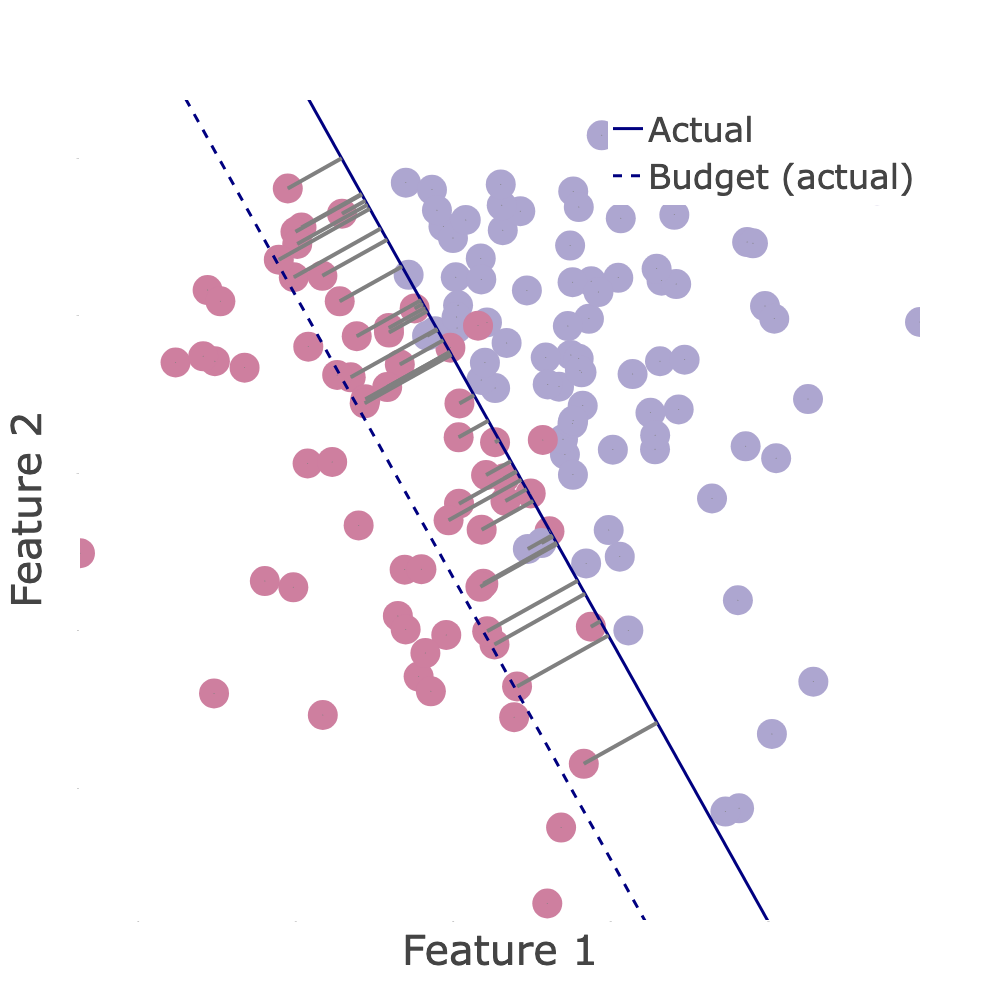
\includegraphics[width=0.82\textwidth]{Figures/NB_movement_arrows.png}
            \caption{Rational strategic response}
            \Description[Rational strategic response]{This figure shows the rational response of agents to a known threshold classifier in 2 dimensions.}
        \label{fig:NB-arrows}
    \end{subfigure}
    \begin{subfigure}[t]{0.3\textwidth}
        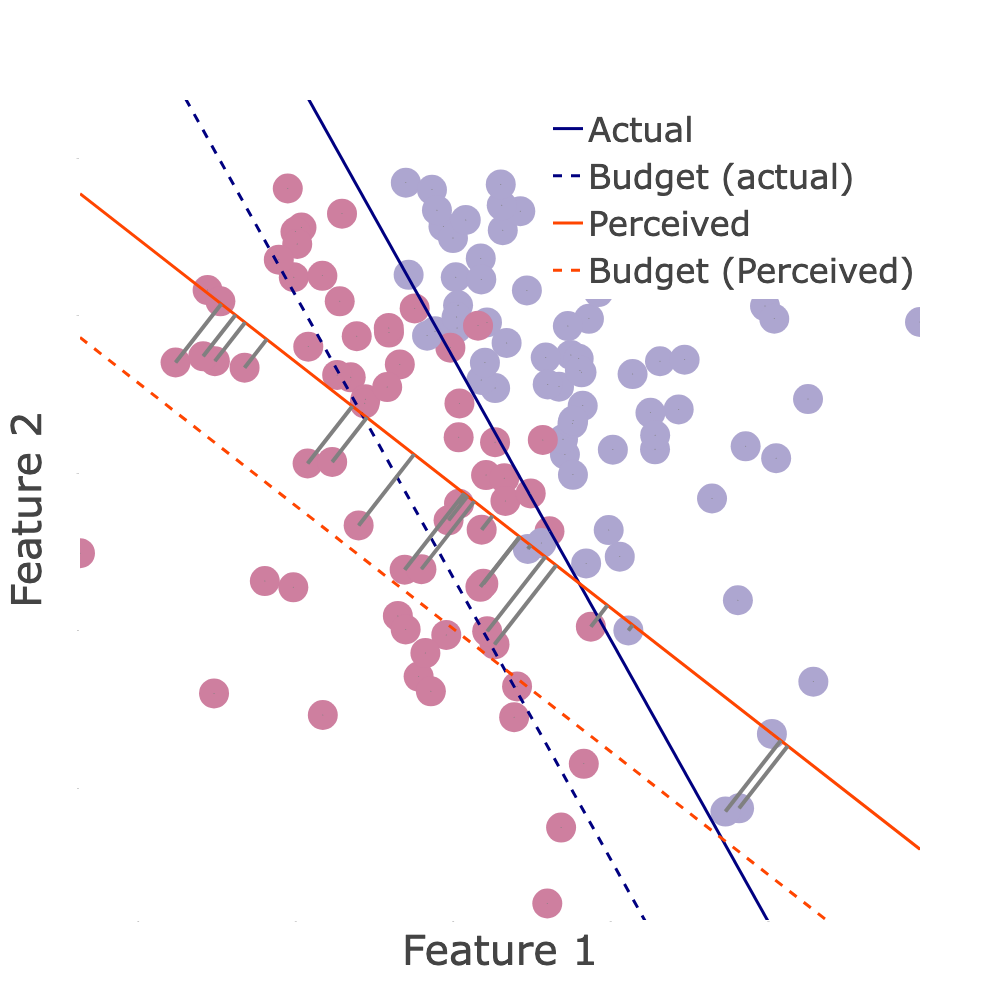
\includegraphics[width=0.82\textwidth]{Figures/B_movement_arrows.png}
        \caption{Biased strategic response}
        \Description[Biased strategic response]{This figure shows the biased response of agents to a known threshold classifier in 2 dimensions.}
        \label{fig:B-arrows}
    \end{subfigure}
    \hspace{0.01in}
    \begin{subfigure}[t]{0.3\textwidth}
        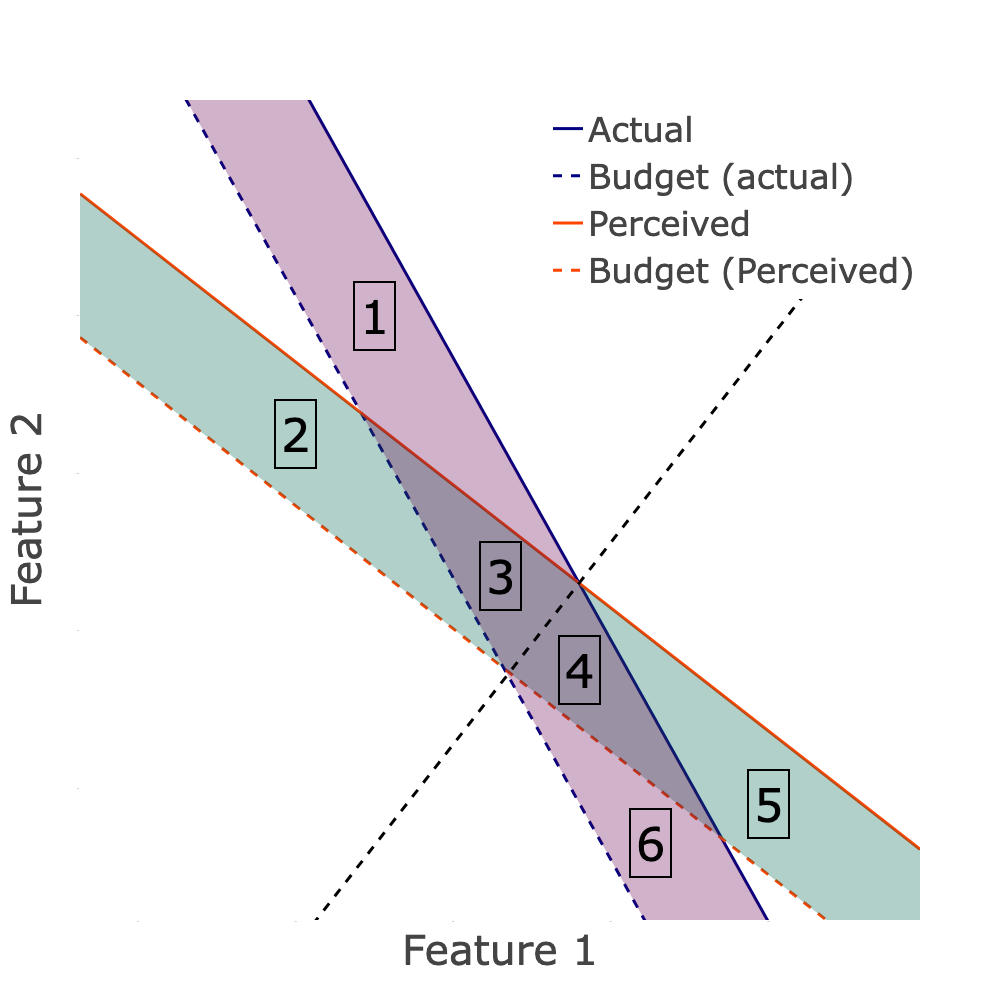
\includegraphics[width=0.82\textwidth]{Figures/B_highlighted_regions.png}
            \caption{Differing strategic responses}
            \Description[Differing strategic response]{This figure shows the regions for the differences between the response of biased and rational agents to a known threshold classifier in 2 dimensions.}
        \label{fig:highlighted}
    \end{subfigure}
    \caption{(a) Fully rational responses, (b) Behaviorally biased responses, and (c) Classes of differing actions. (norm-2 costs)}
    \Description[Rational and biased strategic response]{This figure shows an example of biased and rational response to an algorithm in 2 dimensions.}
    \label{fig:BR-illustration}
\end{figure*} 

We first fix the classifier $(\vtheta, \theta_0)$, and compare fully rational (non-behavioral) and behavioral agents' strategic responses to it. The following Lemma characterizes $\vx_\text{NB}$ (the solution to the optimization problem in \eqref{eq:agent-optimization}) and $\vx_\text{B}$ (the solution to the optimization problem in \eqref{eq:agent-optimization-behavioral}) under the norm-2 cost. All proofs are included in Appendix~\ref{sec:app-proofs}. 


\begin{lemma}\label{lemma:band-optimization}
    Let $d(\vx_0, \vtheta, \theta_0)=\frac{\theta_0-\vtheta^T\vx_0}{\norm{\vtheta}_2^2}$  denote $\vx_0$'s distance to the hyperplane $\vtheta^T\vx=\theta_0$. Then, for an agent with starting feature vector $\vx_0$, if $0 < d(\vx_0, \vtheta, \theta_{0}) \le B$, 
    \begin{align*}
        \vx_\text{NB} = \vx_0 + d(\vx_0, \vtheta, \theta_{0})\vtheta~.%\\
    \end{align*}
    Otherwise, $\vx_\text{NB} = \vx_0$. For behaviorally biased agents, $\vx_{B}$ is obtained similarly by replacing $\vtheta$ with $\vw(\vtheta)$.
\end{lemma}

Figure~\ref{fig:BR-illustration} illustrates the strategic agents' best-responses of Lemma~\ref{lemma:band-optimization}, in a two-dimensional feature space, when they are non-behavioral (Fig.~\ref{fig:NB-arrows}) and when they are behavioral (Fig.~\ref{fig:B-arrows}). We first note that the subset of agents with non-trivial responses to the classifier, as identified in  Lemma~\ref{lemma:band-optimization}, are in a band below the decision boundary. Given the overlaps of these bands under non-behavioral and behavioral responses, there are 6 regions of interest where biased agents' best-responses differ from rational agents (Fig.~\ref{fig:highlighted}). In regions \framebox(7,9){1} and \framebox(7,9){6}, agents invest no effort in manipulating their features when they are behaviorally biased, whereas they do when fully rational; the reasons differ: agents in \framebox(7,9){1} believe they are accepted without effort, while those in \framebox(7,9){6} believe they do not have sufficient budget to succeed. Agents in regions \framebox(7,9){2} and \framebox(7,9){5} manipulate their features unnecessarily (they would not, had they been fully rational), and again, for different reasons: agents in \framebox(7,9){2} are not accepted even at their highest effort level, while those in \framebox(7,9){5} believe they must reach the boundary but they would be accepted regardless of their effort. Finally, in region \framebox(7,9){3}, agents \emph{undershoot} the actual boundary (i.e., exert less effort than needed due to their biases), while those in region \framebox(7,9){4} \emph{overshoot} (i.e., exert more effort than needed to get accepted). 


In the following proposition, we further investigate best-responses in region \framebox(7,9){4} (resp. region \framebox(7,9){3}) and identify which features behavioral agents over-invest in (resp. under-invest in) that leads to them overshooting (resp. undershooting) past the true classifier $(\vtheta, \theta_0)$. 
\begin{proposition}\label{prop:under-invest-high-dim}
Consider an agent with features $\vx_0$, facing classifier $(\vtheta, \theta_0)$, and with a misperceived $\vw(\vtheta)$. Let $\theta_{\max}=\max_i \theta_i$, $d(\vx_0, \vtheta, \theta_0)=\frac{\theta_0-\vtheta^T\vx_0}{\norm{\vtheta}_2^2}$, and  $\delta^{\text{NB}}_i=x_{\text{NB},i}-x_{0,i}$ and $\delta^{\text{B}}_i=x_{\text{B},i}-x_{0,i}$ denote the changes in feature $i$ after best-responses. Then:\\[2pt]
    \hspace*{0.1in}{\textbf{(1)}} If $d(\vx_0, \vw(\vtheta), \theta_0)\le d(\vx_0, \vtheta, \theta_0)$ and $w(\theta_i)<\theta_i$, then $\delta_i^{\text{B}}<\delta_i^{\text{NB}}$.\\[2pt]
    \hspace*{0.1in}\textbf{(2)} If $d(\vx_0, \vtheta, \theta_0)\le d(\vx_0, \vw(\vtheta), \theta_0)$ and $\theta_i<w(\theta_i)$ then $\delta_i^{\text{NB}}<\delta_i^{\text{B}}$.\\[2pt]
    \hspace*{0.1in}\textbf{(3)} For the special case of a Prelec function, we further have: If $d(\vx_0, \vtheta, \theta_0) \le e^{\gamma^\frac{1}{1-\gamma}-\gamma^\frac{\gamma}{1-\gamma}} d(\vx_0, \vw(\vtheta), \theta_0)$ and $w(\theta_{\max})<\theta_{\max}$, then
    $\delta_{\max}^{\text{NB}}<\delta_{\max}^{\text{B}}$. 
\end{proposition}

Intuitively, the proposition states that agents who perceive the decision boundary to be closer to them than it truly is (regions \framebox(7, 9){2} and \framebox(7, 9){3} in Figure~\ref{fig:highlighted}) will under-invest in the features for which they underestimate the importance. Similarly, agents that perceive the boundary to be farther (regions \framebox(7, 9){4} and \framebox(7, 9){5} in Figure~\ref{fig:highlighted}) will over-invest in the features for which they overestimate the importance. 

\section{Firm's Response}\label{sec:firm-response}

We next consider the firm's optimal choice of a classifier, given agents' strategic responses, and its impact on the firm's utility and agents' welfare. Intuitively, one might expect a firm to ultimately benefit from agents' behavioral responses (in contrast to fully rational responses) as behavioral agents are less adept at gaming the algorithm. However, in this section, we show that this is not always true. Intuitively, as demonstrated in Section~\ref{sec:agetns-response}, behavioral agents may overshoot or undershoot the threshold when gaming the algorithm (compared to rational agents); this includes both qualified (label 1) and unqualified (label 0) agents. We show that there exist scenarios in which a relatively higher number of behaviorally biased qualified agents end up below the threshold (due to not trying or undershooting) while relatively more unqualified agents overshoot and end up accepted by the classifier; the combination of these factors can decrease the firm's utility. In other words, perhaps unexpectedly, in these situations, the firm would prefer rational agents, who are better at gaming the system, to behaviorally biased agents, who are worse at gaming the system. 
The following example numerically illustrates this. % possibility. 

\begin{example}\label{ex:firm-benefit-hurt}
Consider a setting where we have a 2D feature space and qualified (resp. unqualified) agents are sampled from a normal distribution $\mathcal{N}(\vmu_{1}, \Sigma_1)$ (resp. $\mathcal{N}(\vmu_0, \Sigma_0)$). We consider three scenarios; the first two scenarios only differ in the mean $\vmu_{1}$ choice, and the third scenario differs with these in $\vmu_{1}$, $\Sigma_1$, $\Sigma_0$, and $B$ (see Appendix~\ref{sec:app-numerical-details} for details). The first two scenarios (top and middle rows in Figure~\ref{fig:firm-benefit-hurt-dist}) are baselines: we consider an \emph{oblivious} firm that chooses its classifier without accounting for any strategic response (whether rational or behavioral) from agents. This helps us hone in on the impacts of agents' qualification states on the firm's utility. Then, in the third scenario (bottom row in Figure~\ref{fig:firm-benefit-hurt-dist}), we consider a firm that is aware of strategic behavior (and any behavioral biases) by agents and optimally adjusts its classifier. For each scenario, Figure~\ref{fig:firm-benefit-hurt-dist} illustrates the distribution of agents' features for pre-strategic (left panel), post-strategic non-behavioral responses (middle panel), and post-strategic behaviorally-biased responses (right panel). The firm's utility in each case is shown at the top of the corresponding subplot.

\begin{figure*}[t]
    \centering
    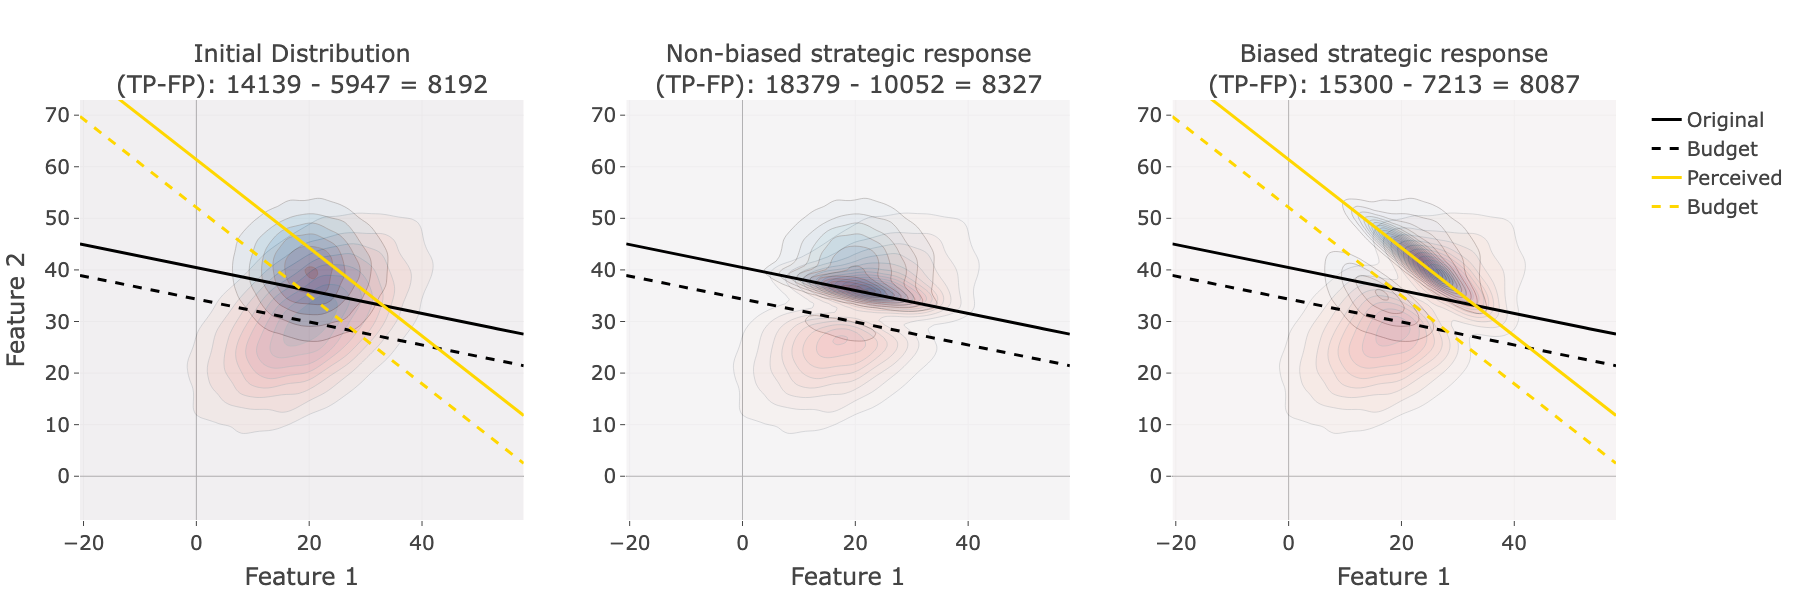
\includegraphics[width=0.9\linewidth]{Figures/1_all_three_GOATEDPLOT1_firm_gets_hurt.png}
    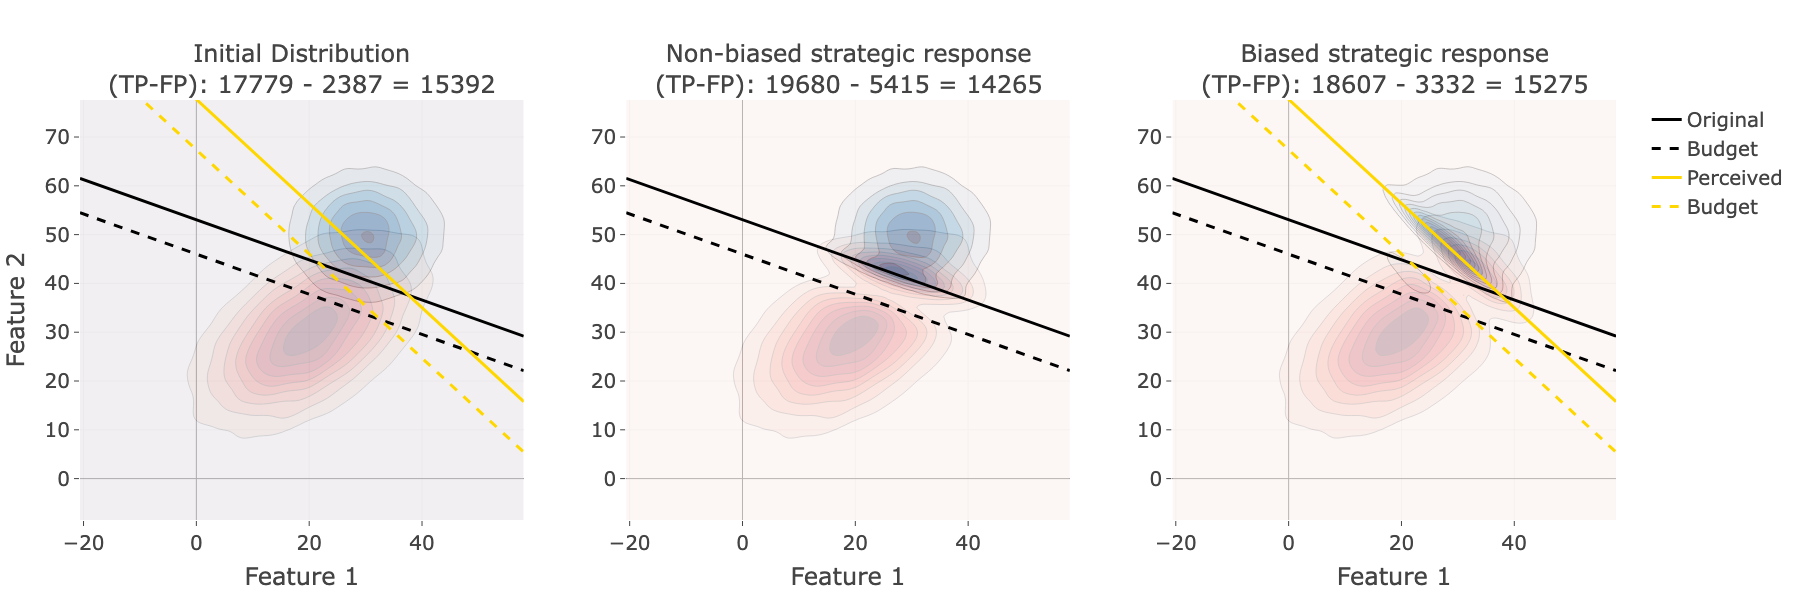
\includegraphics[width=0.9\linewidth]{Figures/1_all_three_GOATEDPLOT2_firm_benefits.png}
    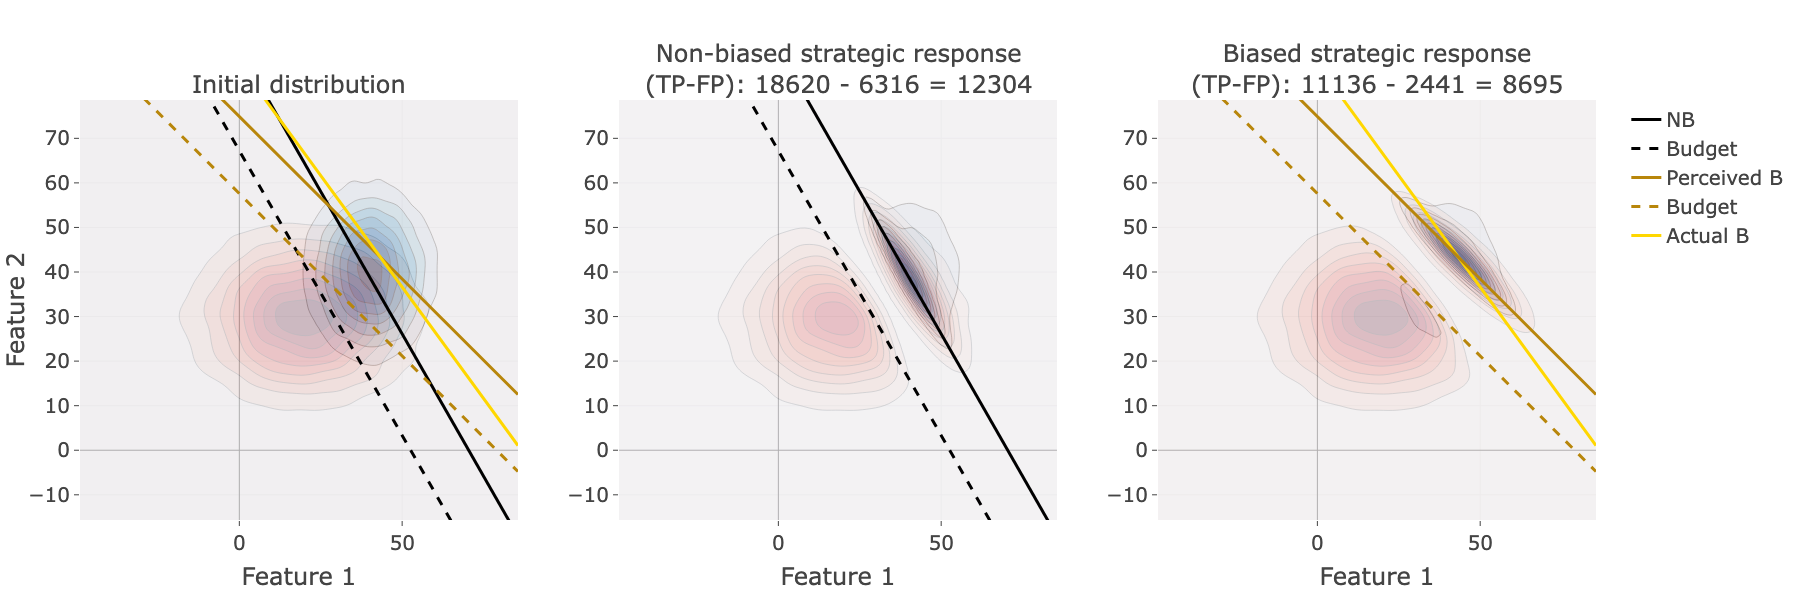
\includegraphics[width=0.9\linewidth]{Figures/1_all_three_GOATEDPLOT_nonoblivious_firm.png}
    \caption{An oblivious firm may have lower (top) or higher (middle) utility when agents are biased (vs. rational). A non-oblivious firm may still have a lower utility when agents are biased (bottom). {The firm's utility is shown above the subplots as (\#TP-\#FP).}}
    \Description[Different scenarios occurring in an example]{An oblivious firm may have lower (top) or higher (middle) utility when agents are biased (vs. rational). A non-oblivious firm may still have a lower utility when agents are biased (bottom).}
    \label{fig:firm-benefit-hurt-dist}
\end{figure*}

We start with the baselines (an oblivious firm that keeps the classifier fixed). In the top row scenario, the firm is negatively impacted by agents' behavioral biases, while in the middle row scenario, the firm benefits from agents' biases (both compared to the fully rational setting). The reason for this difference is that there are more qualified agents than unqualified ones who reach the threshold in non-biased responses. On the other hand, under biased responses, there are more unqualified agents who pass the threshold, regardless of their bias (those in region \framebox(7, 9){3} in Fig.~\ref{fig:highlighted}) in the top row scenario. Behavioral responses by these agents negatively impact the firm, as it leads to these qualified agents no longer being accepted. 

Next, we consider the (non-oblivious) firm that adjusts its classifier optimally (accounting for strategic responses \emph{and} behavioral biases, if any). We observe that even though the firm is aware of agents' bias, its loss is higher than the case of rational responses. As seen in the left panel of the bottom row of Figure~\ref{fig:firm-benefit-hurt-dist}, more regions can impact the loss than in Figure~\ref{fig:BR-illustration}. The most important regions in this scenario are the areas accepted by $\vtheta_\text{NB}$ but not by $\vtheta_\text{B}$ (after response), and vice versa. As there are more qualified than unqualified agents in these two regions, the firm is negatively impacted by agents' bias (compared to fully rational agents) even though the firm is aware of the bias.

\end{example}

The next proposition formalizes the above intuition. 

\begin{proposition}\label{prop:mismatch-actual-b} 
    Consider a loss function $l(\vx, (\vtheta, \theta_0))=-u^+\text{TP}+u^-\text{FP}$. Let the pdf of label $y$ agents' feature distribution be $f_y(\vx)$, and the number of label $y$ agents be $\alpha_0$. Let $\mathcal{H}(\vtheta, \theta_0)$ denote the set of agents that satisfy $(1-\sigma(\vtheta))\theta_0\le(\vtheta-\sigma(\vtheta)\vw(\vtheta))^T\vx$, where $\sigma(\vtheta) \coloneqq \frac{\vtheta^T\vw(\vtheta)}{\norm{\vw(\vtheta)}^2}$\footnote{Note that $\sigma(\vtheta)=\frac{\norm{\vtheta}_2}{\norm{\vw(\vtheta)}_2}\cos(\alpha)$ where $\alpha$ is the angle between the actual and perceived decision boundaries. The larger $\alpha$ is, the lower $\sigma(\vtheta)$ is, indicating a more intense bias.}, and the set of agents that attempt to game the algorithm as $\sA(\vtheta, \theta_0) = \{\vx_0: \theta_0 - B \le \vtheta^T\vx_0 < \theta_0 \}$. Denote the set of accepted (resp. rejected) agents by $(\vtheta, \theta_0)$ with $\sY(\vtheta, \theta_0)$ (resp. $\sN(\vtheta, \theta_0)$). Define the sets 
    \begin{align*}        
        &\sS(\vtheta_\text{NB}, \theta_{0, \text{NB}}) \coloneqq \sA(\vtheta_\text{NB}, \theta_{0, \text{NB}})/(\sA(\vtheta_\text{NB}, \theta_{0, \text{NB}})\cap\mathcal{H}(\vtheta_\text{NB}, \theta_{0, \text{NB}})), \\
        &\sT_1=(\sY(\vtheta_\text{NB}, \theta_{0,\text{NB}})\cup \sA(\vtheta_\text{NB}, \theta_{0,\text{NB}}))\cap \sN(\vtheta_\text{B}, \theta_{0,\text{B}})\text{, and} \\
        &\sT_2 = (\mathcal{H}(\vtheta_\text{B}, \theta_{0,\text{B}})\cap \sA(\vw(\vtheta_\text{B}), \theta_{0,\text{B}}))\cup \\
        &\hspace{1cm}((\sY(\vtheta_\text{B}, \theta_{0,\text{B}}) \cap \sN(\vtheta_\text{NB}, \theta_{0,\text{NB}}))/\sA(\vtheta_\text{NB}, \theta_{0,\text{NB}})).
    \end{align*}
    Then:\\[2pt]
    \hspace*{0.1in}{\textbf{(a)}} If $\int_{x\in \sS(\vtheta_\text{NB}, \theta_{0, \text{NB}})} u^- f_0(\vx)\alpha_0 d\vx \le \int_{x\in \sS(\vtheta_\text{NB}, \theta_{0, \text{NB}})} u^+ f_1(\vx)\alpha_1 d\vx $ we can say: 
    \begin{align}\label{eq:firm-loss-comp-benefit}
        \sL(\vw(\vtheta_\text{B}), (\vtheta_\text{B}, \theta_{0, \text{B}}))&\le \sL(\vw(\vtheta_\text{NB}), (\vtheta_\text{NB}, \theta_{0, \text{NB}}))\notag \\
        &\le \sL(\vtheta_\text{NB}, (\vtheta_\text{NB}, \theta_{0, \text{NB}}))
    \end{align}
    \hspace*{0.1in}{\textbf{(b)}} If $\int_{x\in \sS(\vtheta_\text{NB}, \theta_{0, \text{NB}})} u^+ f_1(\vx)\alpha_1 d\vx \le \int_{x\in \sS(\vtheta_\text{NB}, \theta_{0, \text{NB}})} u^- f_0(\vx)\alpha_0 d\vx $ we can say: 
    \begin{align}\label{eq:firm-loss-comp-hurt}
        \max\{\sL(\vtheta_\text{NB}, (\vtheta_\text{NB}, \theta_{0, \text{NB}}))&,\; \sL(\vw(\vtheta_\text{B}), (\vtheta_\text{B}, \theta_{0, \text{B}}))\}\notag\\
        &\le \sL(\vw(\vtheta_\text{NB}), (\vtheta_\text{NB}, \theta_{0, \text{NB}}))
    \end{align}
    \hspace*{0.1in}{\textbf{(c)}} If $\int_{\vx\in\sT_1}(-u^+f_1(\vx)\alpha_1+u^-f_0(\vx)\alpha_0)d\vx \le \int_{\vx\in\sT_2}(-u^+f_1(\vx)\alpha_1+u^-f_0(\vx)\alpha_0)d\vx$ we can say:
    \begin{align}\label{eq:firm-loss-comp-hurt-NB-B}
        \sL(\vtheta_\text{NB}, (\vtheta_\text{NB}, \theta_{0, \text{NB}}))&\le \sL(\vw(\vtheta_\text{B}), (\vtheta_\text{B}, \theta_{0, \text{B}}))\notag\\
        &\le \sL(\vw(\vtheta_\text{NB}), (\vtheta_\text{NB}, \theta_{0, \text{NB}}))
    \end{align}
\end{proposition}
Part (a) states that if a firm is unaware of agents' behavioral biases, it will suffer a lower loss when the population is biased compared to fully rational. This is the intuitively expected scenario (behaviorally biased agents are less adept than fully rational ones at gaming the algorithm). On the other hand, statement (b) reflects the less expected outcome: a firm unaware of behavioral biases will have \emph{lower} utility when agents are biased compared to if they had been fully rational (as more \emph{qualified} than \emph{unqualified} agents undershoot the threshold under this case's condition). Statement (c) further compares the unaware firm with an aware firm and provides a condition where an aware firm's minimal loss is higher than the non-biased minimal loss. This condition relies on the \emph{difference} of qualified and unqualified agents in two regions.
Lastly, we note that even though $\vw(\cdot)$ is not directly seen in the conditions of Proposition~\ref{prop:mismatch-actual-b}, it affects the regions in which the conditions are satisfied. Generally, the influence of weighting functions, such as Prelec function, on $\vtheta$ can be described as $\vw(\vtheta) = \vtheta + \vbeta$ where $\vbeta$ satisfies two conditions: (1) $\sum_i \beta_i = 0$ ensuring that $\sum_i w_i(\vtheta) = 1$ and implying that increasing the perceived importance of one feature necessarily requires under-estimating at least one other feature and (2) $0\le \theta_i + \beta_i \le 1$ ensuring that the adjusted weights remain within the range $[0,1]$. Therefore, the general impact of other forms of $\vw(\cdot)$ will be similar to Prelec function.

\subsection{Impact on Agents' Welfare}\label{sec:agents_welfare}
We end this section by comparing the impacts of behavioral biases on agents' welfare (sum of their utilities). As a baseline, note that if the firm was oblivious to agents' strategic responses and did not adjust the classifier, agents would have lower welfare when they are behaviorally biased (compared to when rational). This is an expected outcome since behaviorally biased agents are worse at gaming the algorithm and respond sub-optimally. But, perhaps more unexpectedly, when the firm adjusts its classifier in response to agents' strategic behavior and behavioral biases, various scenarios can occur, in some of which behavioral agents obtain \emph{higher} welfare than if they had been rational. For instance, in the bottom row of Figure~\ref{fig:firm-benefit-hurt-dist}, qualified agents have \emph{higher} social welfare when they are behaviorally biased compared to if they had been rational. We provide additional intuition for reasons for this in a 2-D feature space example below. %in Appendix~\ref{app:welfare}. 

Figure~\ref{fig:SW-regions} highlights the change in utility when agents are behaviorally biased (vs. when they were rational) across different regions in the feature space, with the regions generated based on the firm's optimal choice of threshold and agents' responses to it. In particular, the utility of agents in the green-highlighted region (this is $\sY(\vtheta_\text{B}, \theta_{0,\text{B}}) \cap \sN(\vtheta_\text{NB}, \theta_{0,\text{NB}})$ in Proposition~\ref{prop:mismatch-actual-b}) increases when they are behaviorally biased. One subset of agents in this region are those 
%$\sY(\vtheta_\text{B}, \theta_{0,\text{B}}) \cap \sN(\vtheta_\text{NB}, \theta_{0,\text{NB}})\cap \sA(\vtheta_\text{NB}, \theta_{0, \text{NB}})$ where 
who in the rational case exert effort to get admitted and have a utility $r-c(\vx,\vx_0)$, whereas in the behaviorally biased case they attain utility $r > r-c(\vx,\vx_0)$ as they get admitted without any effort (and they correctly assume so). Another one is %subset is $(\sY(\vtheta_\text{B}, \theta_{0,\text{B}}) \cap \sN(\vtheta_\text{NB}, \theta_{0,\text{NB}}))/\sA(\vtheta_\text{NB}, \theta_{0,\text{NB}})$ which is 
the subset of agents who would not try to get to the decision boundary in the rational case (and so have utility of $0$), but in the behavioral case, they are receiving utility $r$ without any movement and due to the change of the decision boundary. For the numerical example in the bottom row of Figure~\ref{fig:firm-benefit-hurt-dist}, there are more agents in this green-highlighted region than in the remaining red-highlighted regions (where biased agents have lower utility than rational agents), leading to an overall higher welfare for all agents when they are biased compared to when they were rational. 

\begin{figure}[ht]
    \centering
    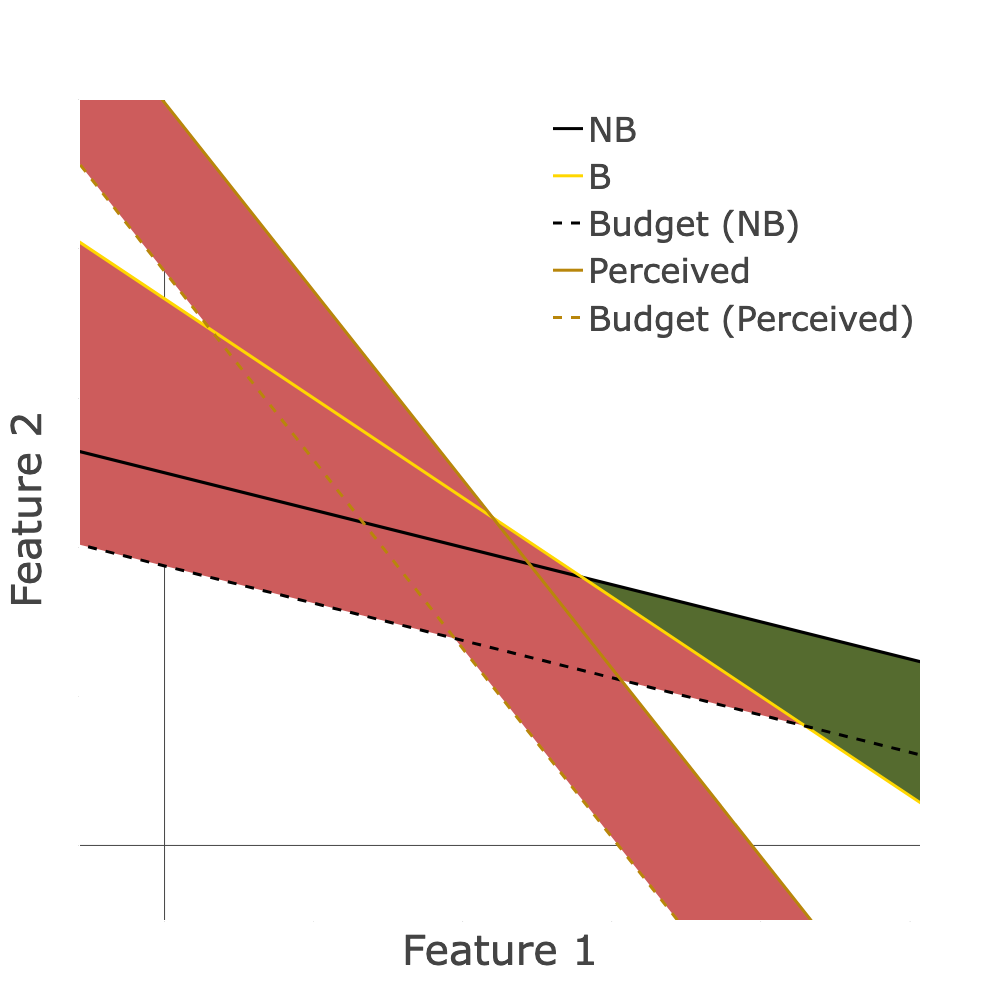
\includegraphics[width=0.6\linewidth]{Figures/SW_highlighted regions.png}
    \caption{Regions where agents have higher (green) or lower (red) utility when biased vs. had they been fully rational.}
    \Description[Welfare regions]{Regions where agents have higher (green) or lower (red) utility when biased vs. had they been fully rational.}
    \label{fig:SW-regions}
\end{figure}


%For B responses, the social welfare for qualified and unqualified agents drops, while unqualified agents get hurt more because they have a higher than necessary or unnecessary cost. 

% Figure~\ref{fig:SW-regions} highlights the change in utility when agents are behaviorally biased (vs. when they were rational) across different regions in the feature space, with the regions generated based on the firm's optimal choice of threshold and agents' responses to it. In particular, the utility of agents in the green-highlighted region (this is $\sY(\vtheta_\text{B}, \theta_{0,\text{B}}) \cap \sN(\vtheta_\text{NB}, \theta_{0,\text{NB}})$ in Proposition~\ref{prop:mismatch-actual-b}) increases when they are behaviorally biased. One subset of agents in this region are those 
% %$\sY(\vtheta_\text{B}, \theta_{0,\text{B}}) \cap \sN(\vtheta_\text{NB}, \theta_{0,\text{NB}})\cap \sA(\vtheta_\text{NB}, \theta_{0, \text{NB}})$ where 
% who in the rational case exert effort to get admitted and have a utility $r-c(\vx,\vx_0)$, whereas in the behaviorally biased case they attain utility $r > r-c(\vx,\vx_0)$ as they get admitted without any effort (and they correctly assume so). Another one is %subset is $(\sY(\vtheta_\text{B}, \theta_{0,\text{B}}) \cap \sN(\vtheta_\text{NB}, \theta_{0,\text{NB}}))/\sA(\vtheta_\text{NB}, \theta_{0,\text{NB}})$ which is 
% the subset of agents who would not try to get to the decision boundary in the rational case (and so have utility of $0$), but in the behavioral case, they are receiving utility $r$ without any movement and due to the change of the decision boundary. For the numerical example in the bottom row of Figure~\ref{fig:firm-benefit-hurt-dist}, there are more agents in this green-highlighted region than in the remaining red-highlighted regions (where biased agents have lower utility than rational agents), leading to an overall higher welfare for all agents when they are biased compared to when they were rational. 

% \begin{figure}[ht]
%     \centering
%     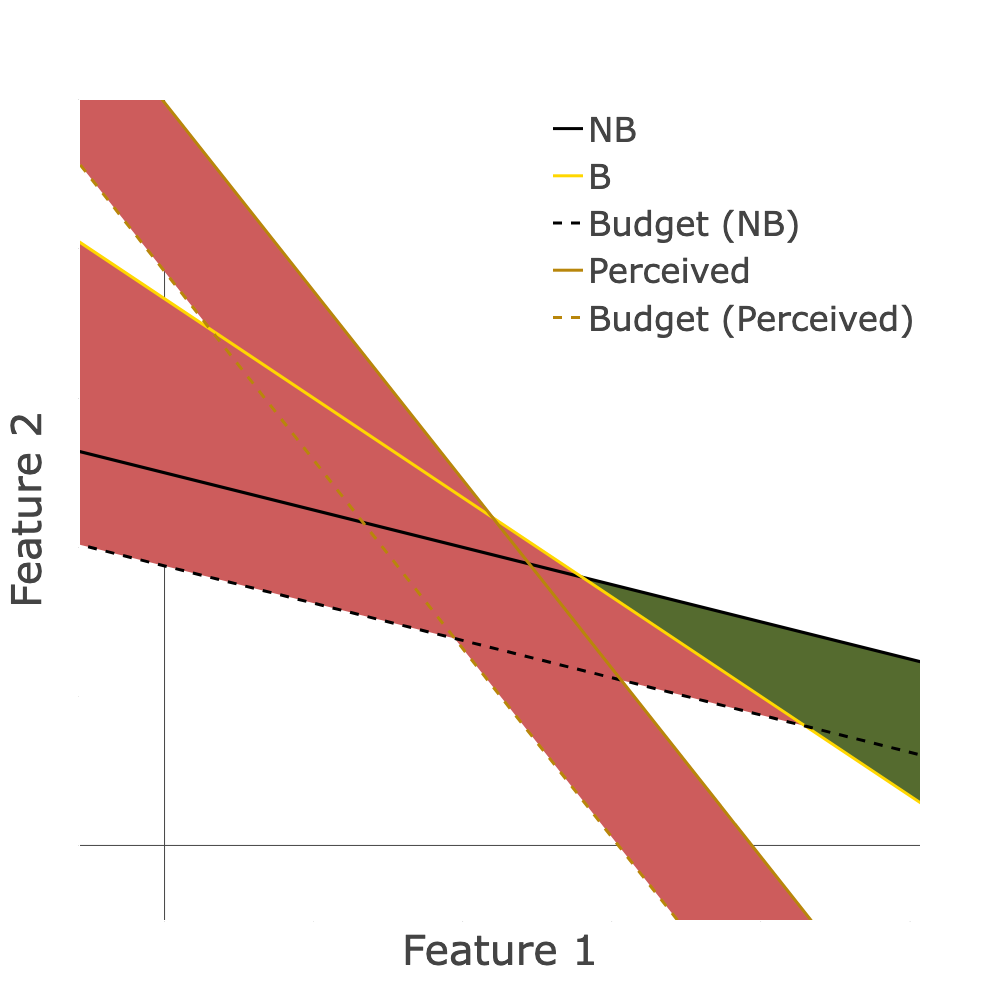
\includegraphics[width=0.5\linewidth]{Figures/SW_highlighted regions.png}
%     \caption{Regions where agents have higher (green) or lower (red) utility when biased vs. when rational.}
%     \label{fig:SW-regions}
% \end{figure}

%In the behavioral case, most regions will not have higher social welfare (Figure~\ref{fig:SW-regions}). Intuitively, for the B case, a firm will ``tilt'' the NB decision boundary to automatically accept more qualified agents and reject more unqualified agents. By this intuition, the firm will see mostly qualified agents in the green region in Figure~\ref{fig:SW-regions} and mostly unqualified agents in the red regions in Figure~\ref{fig:SW-regions}. 

\section{User Study}\label{sec:user-study}
{We next conduct user studies to assess whether and how humans exhibit biases when responding to algorithms. We use the results of these experiments as a proof of concept, shedding light on the existence of misperceptions about algorithm explanations in real-world scenarios, and show that they can be interpreted using our model of feature weight misperceptions. These user studies also help us understand the conditions where our model performs well, as well as settings where our model has shortcomings.}

\subsection{Study Design, Participants, and Setup}\label{sec:study-design}
To understand how human biases affect their responses to algorithms, we conducted a large-scale online survey where participants completed a task with an optimal solution (here, an optimal strategic response to a classifier). We then measured how their answers differed from the optimal solution to assess bias. Similar to previous sections, we focus on how participants perceive the feature weights and how this influences their response to the algorithm. Surveys generally took {5.5} minutes, and participants were paid {\$16 per hour}. The study design was reviewed by our IRB, and the full protocol is included in the supplementary materials. 

\noindent\textbf{Experimental Design.} We used a $2\times2$ between-subjects design, varying the number of features and the feature weights and two contexts. Participants were randomly assigned to a condition and shown a single explanation (shown in Figure~\ref{fig:feature-based-explanations}), with \textit{a}) either two or four features, \textit{b}) either balanced or unbalanced feature weights, and \textit{c}) either familiar or unfamiliar context. 

\noindent\textbf{Procedure.} All participants were shown a truthful and complete explanation from an interpretable ML algorithm. Each participant was asked to complete a task based on the information provided in the explanation. After completing the task, participants were asked questions about their understanding, trust, satisfaction, and performance, common measures in explainability evaluations~\cite{mohseni2021survey}. 

\noindent\textbf{Explanation.} Based on prior work, which has found that feature importance is the most used explanation \cite{systematic2023nauta} and that visualization can help users understand explanations \cite{peeking2018adadi}, we developed an explanation that shows feature weights in a bar graph (Figure~\ref{fig:feature-based-explanations}). The system uses the displayed feature weights as an interpretable ML algorithm. 

\begin{figure*}[ht]
    \centering 
    %KV CHANGED SO ALL IMAGES SAME WIDTH 
    \hspace{.5em}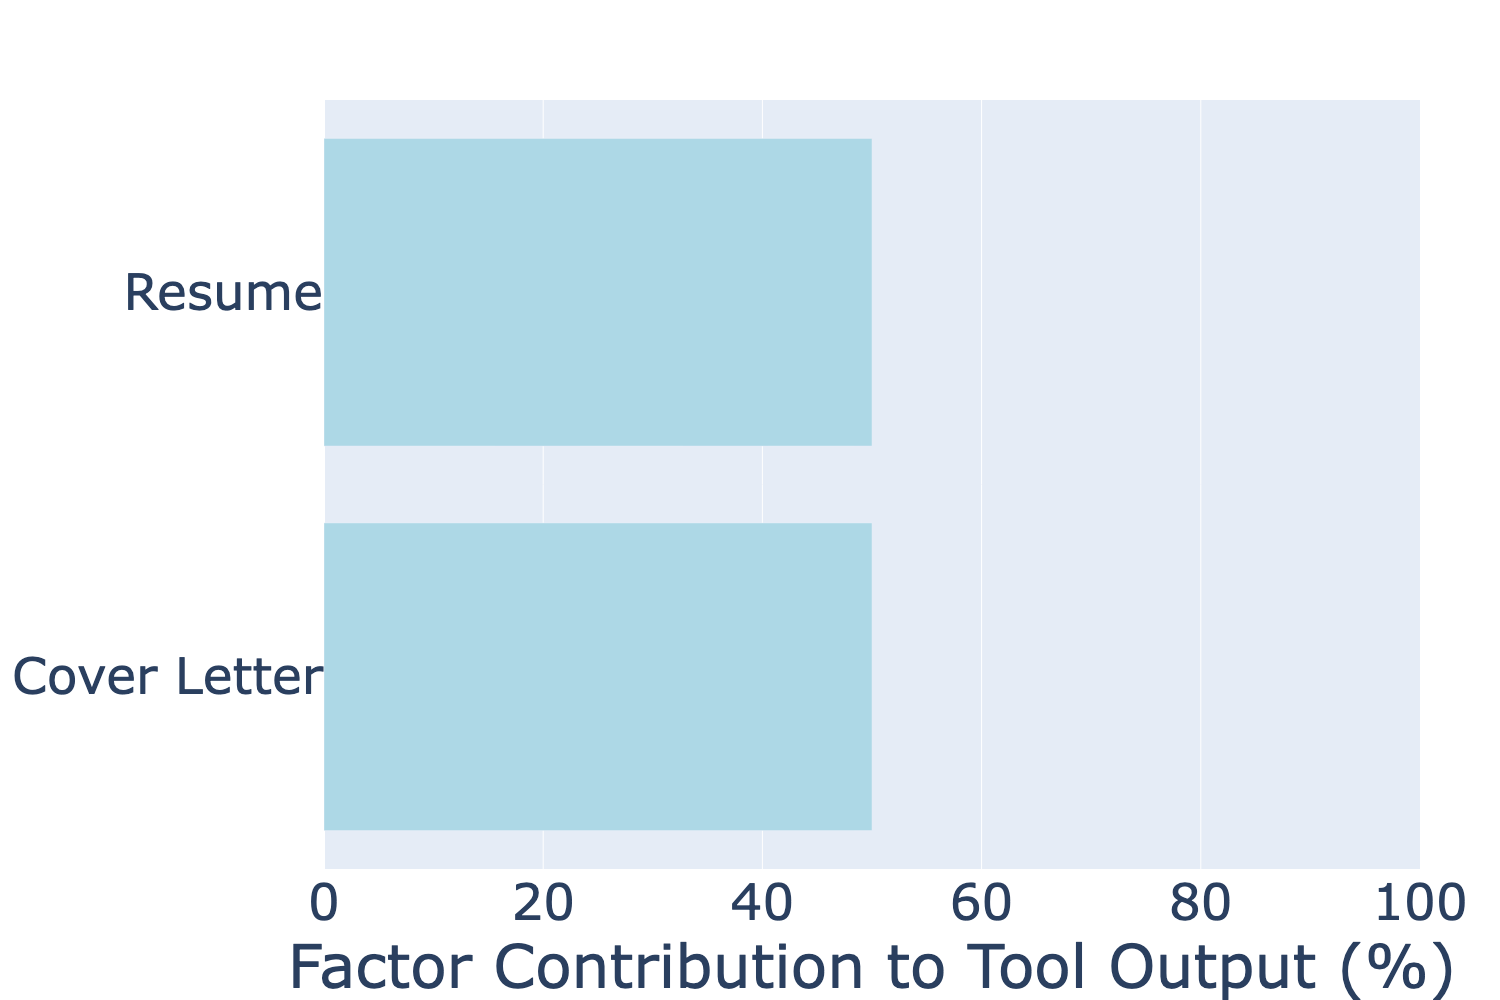
\includegraphics[width=0.245\textwidth]{Figures/2-equal.png}
    \hspace{.5em}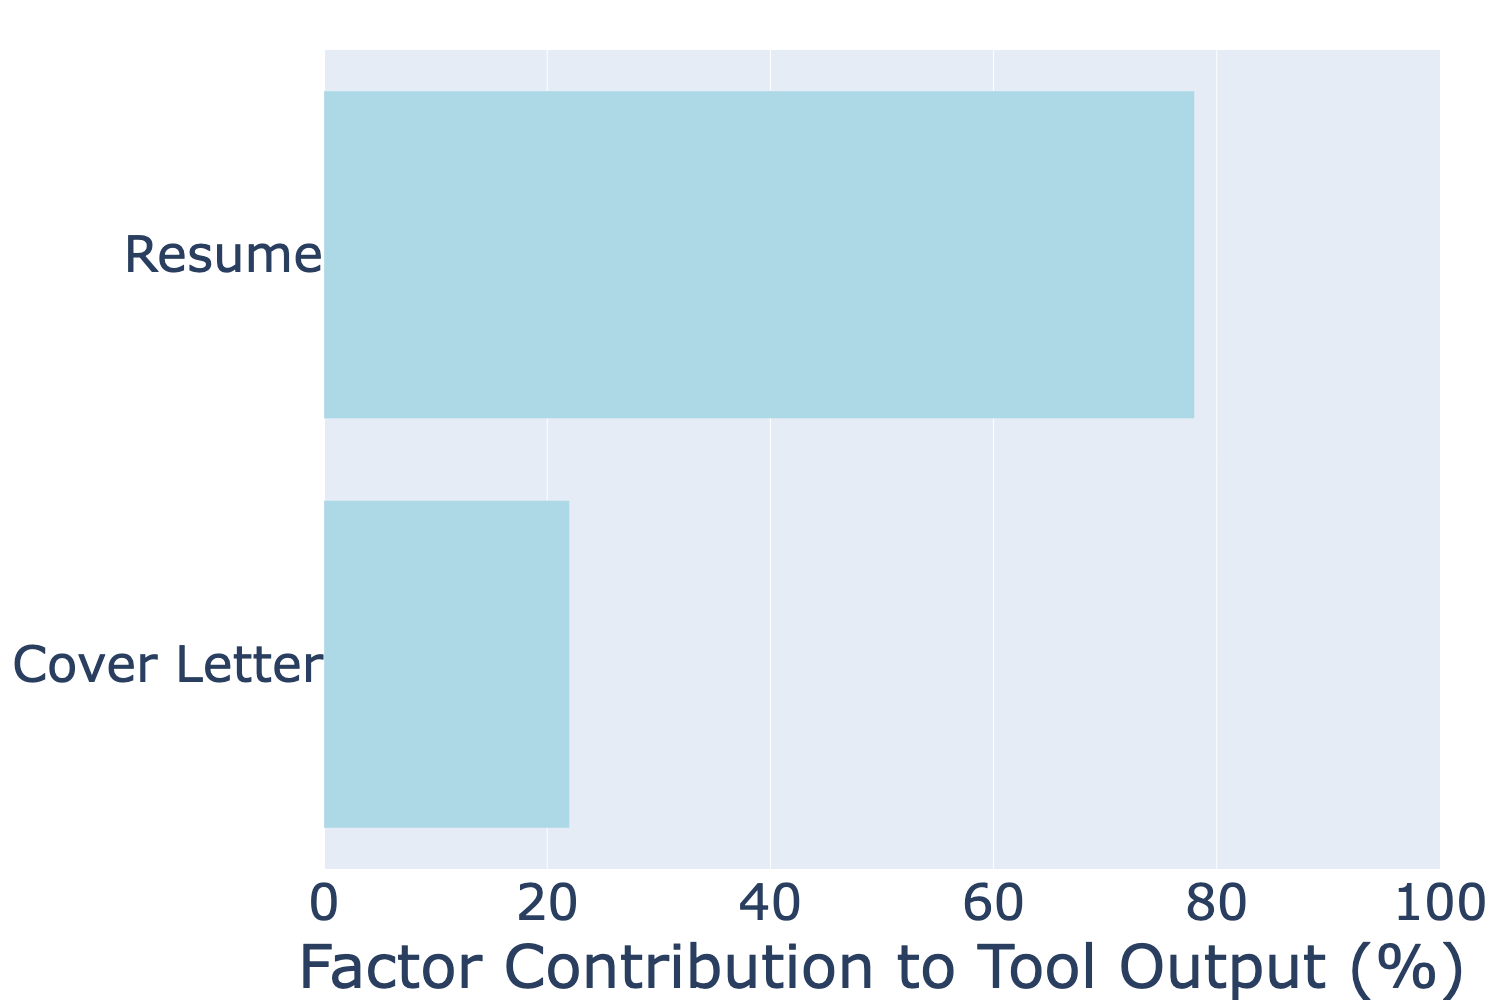
\includegraphics[width=0.24\textwidth]{Figures/2-unequal.png}
    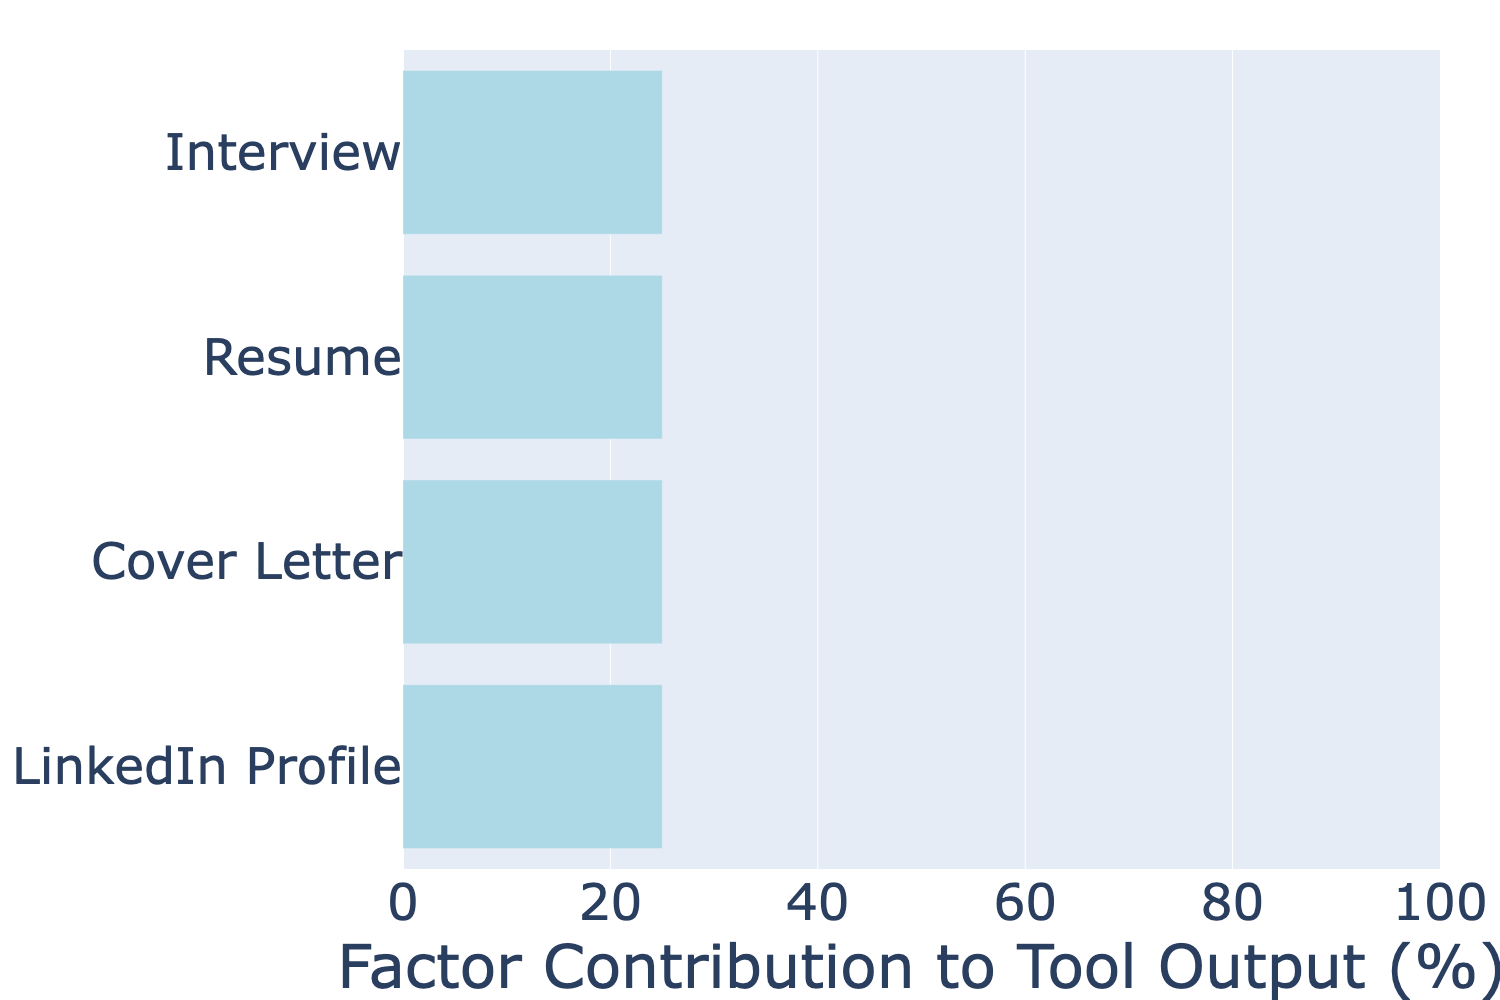
\includegraphics[width=0.24\textwidth]{Figures/4-equal.png}
    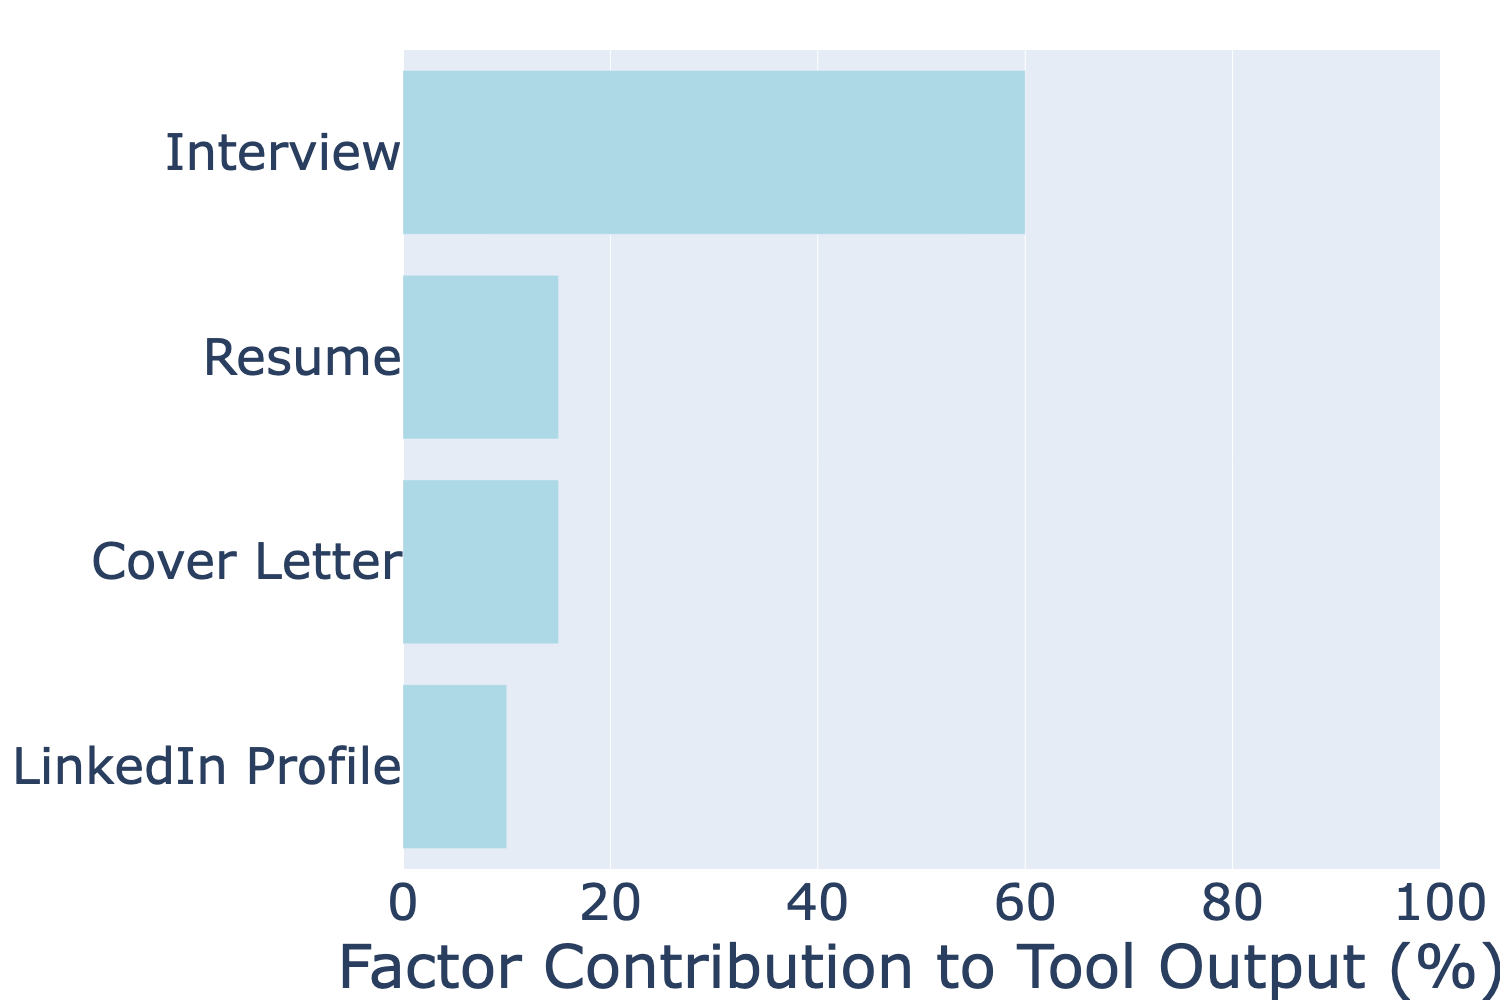
\includegraphics[width=0.24\textwidth]{Figures/4-unequal.png}\\
    \hspace{.5em}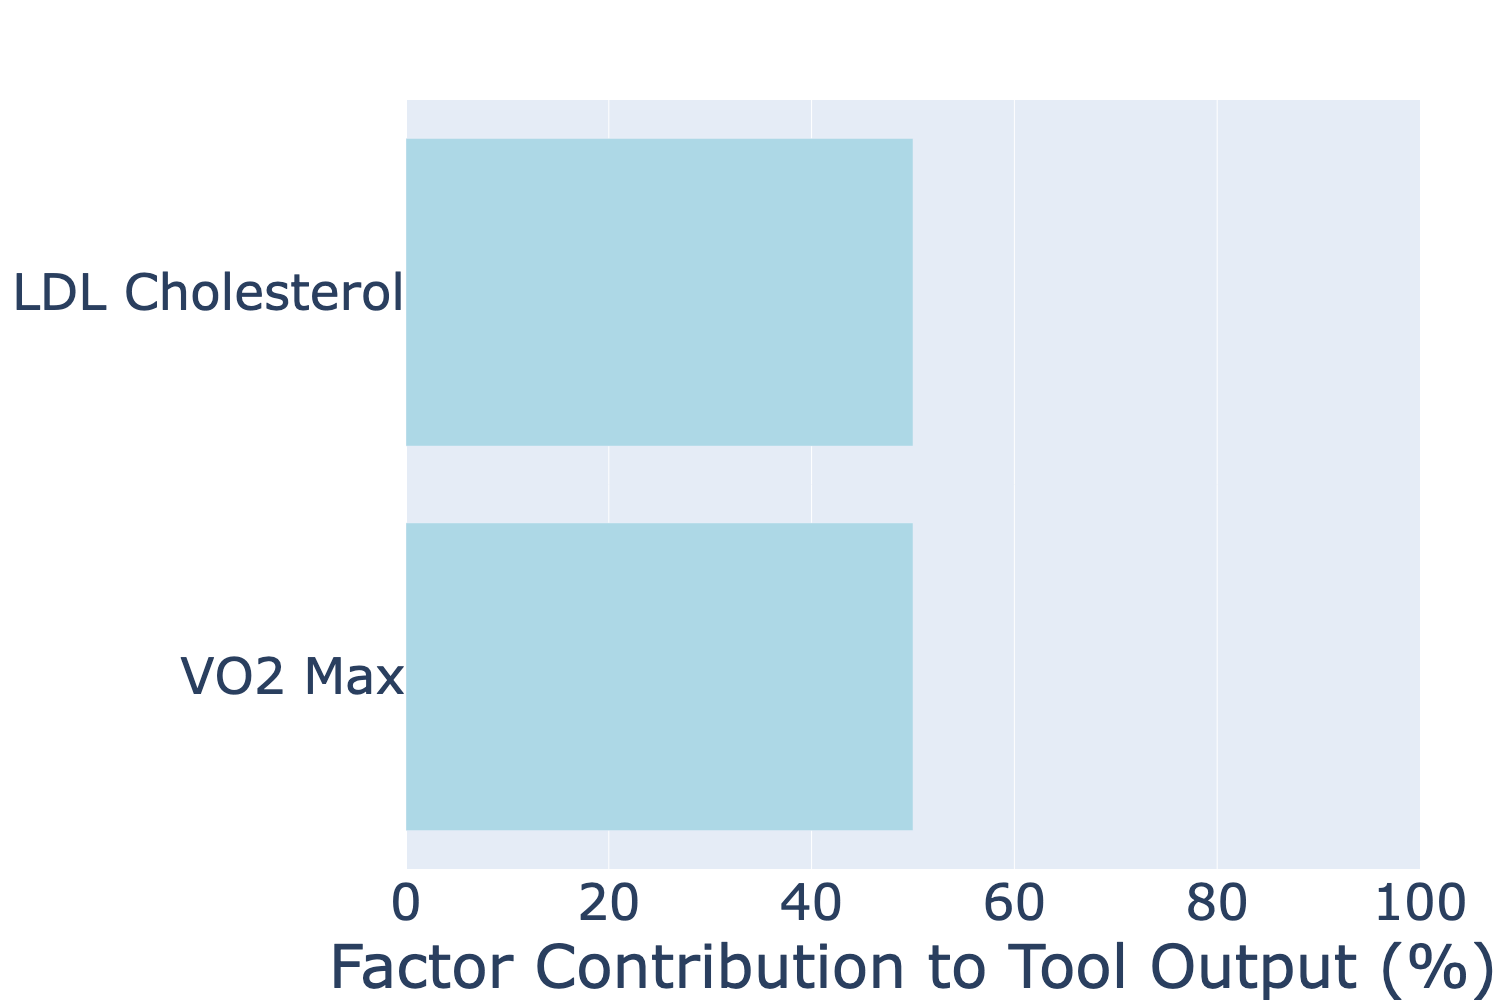
\includegraphics[width=0.245\textwidth]{Figures/2_unf_bal.png}
    \hspace{.5em}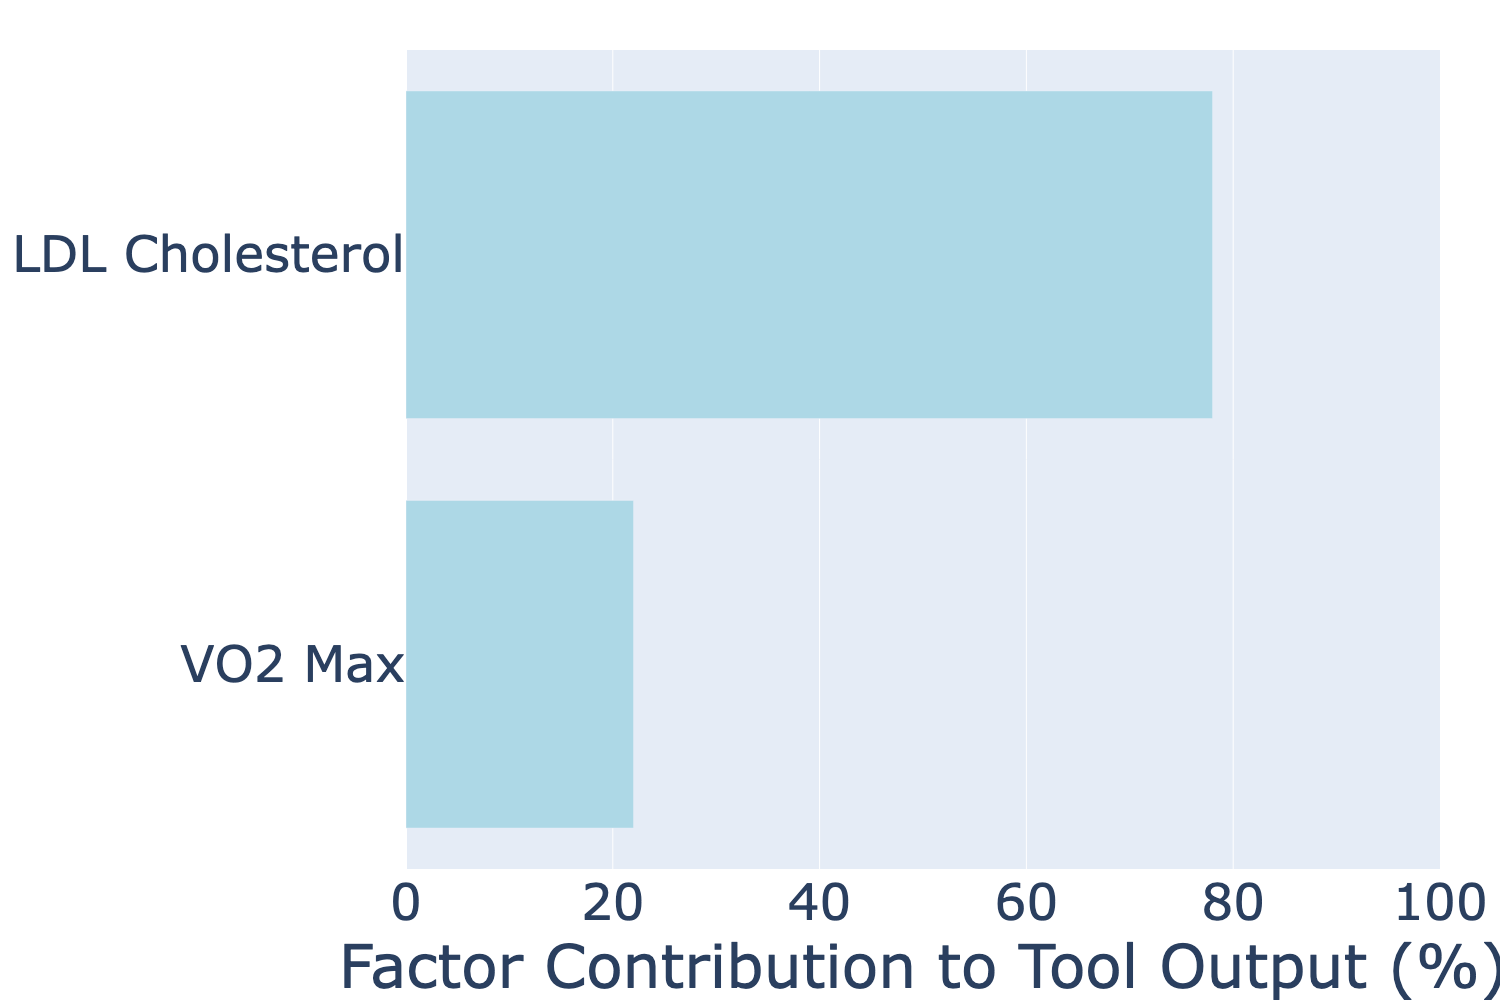
\includegraphics[width=0.24\textwidth]{Figures/2_unf_unbal.png}
    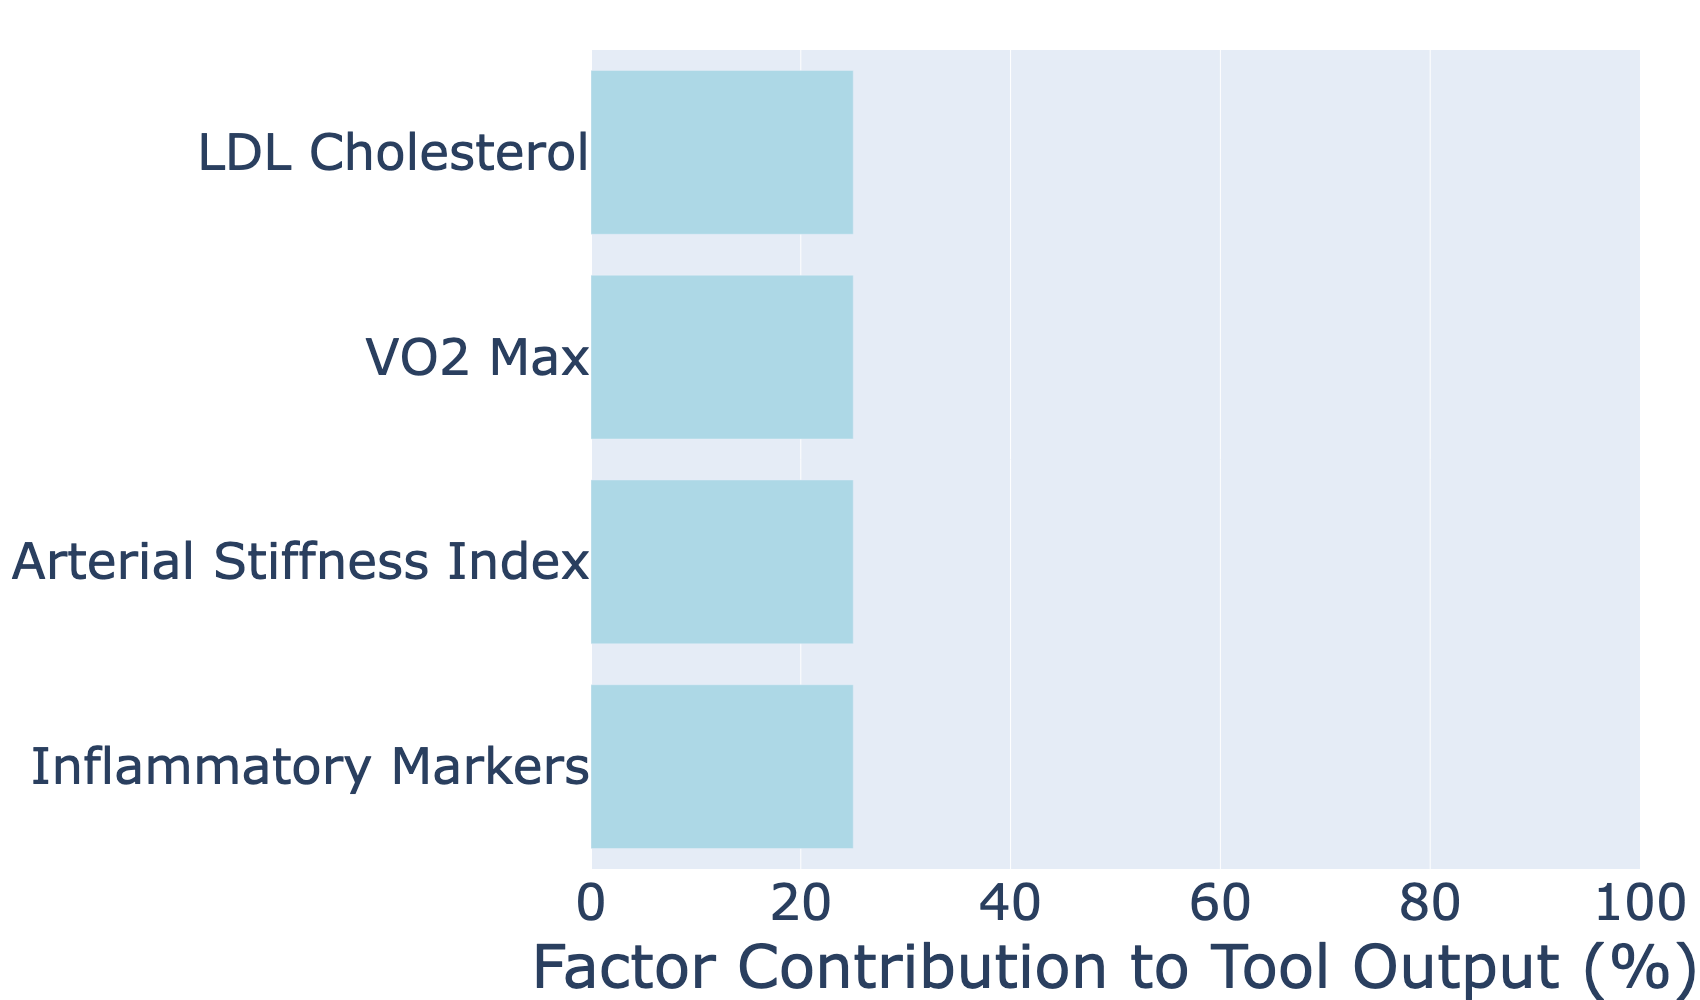
\includegraphics[width=0.24\textwidth]{Figures/4_unf_bal.png}
    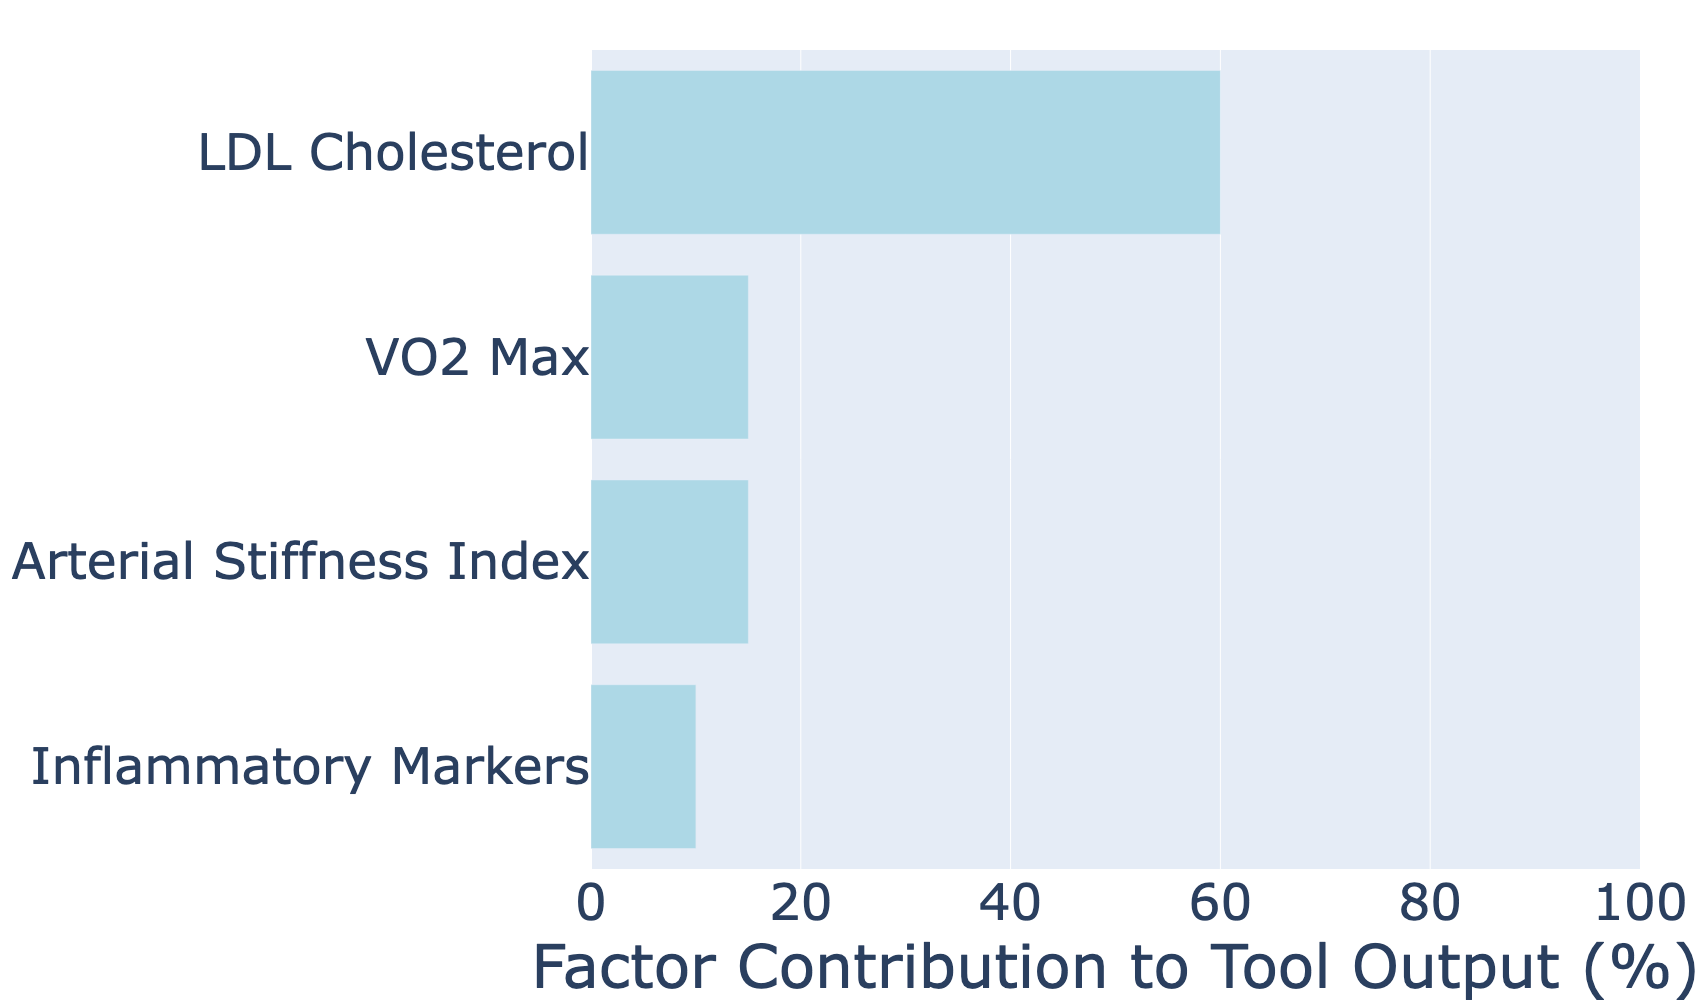
\includegraphics[width=0.24\textwidth]{Figures/4_unf_unbal.png}
    
    \caption{The scenarios shown to participants with familiar context in the first row and unfamiliar context in the second row: two or four features of similar importance (first and third column of figures from the left resp.), and two or four features of differing importance (second and last column of figures from the left resp.).}
    \Description[Survey plots]{The scenarios shown to participants: two or four features of similar importance (top and bottom left resp.), and two or four features of differing importance (top and bottom right).}
    \label{fig:feature-based-explanations}
\end{figure*}


\noindent\textbf{Task.} The familiar task asked participants to give advice to a friend about how to prepare for the job application process. Participants were told an AI system provides predictions of applicants' qualification for the job. The features used by the AI were resume (R) and cover letter (CL), with two additional features, interview (I) and LinkedIn profile (LP), for the four feature conditions. The unfamiliar task asked participants to give a friend advice about how to improve health metrics for a medical test. Participants were told an AI system provides predictions of the likelihood of a major cardiovascular event. The features used by the AI were LDL cholesterol (L) and VO2 max (V), with two additional features, arterial stiffness index (A) and inflammatory markers (I), for the four feature conditions.

Each participant had a budget (10 hours in the familiar context and 10 weeks in the unfamiliar context) to allocate between the given features to improve the likelihood of favorable recommendation. For starting features, in the two-feature and four-feature scenarios, we used $\vx_0=(40, 60)$ and $\vx_0=(60, 40, 60, 65)$, where, the maximum for feature scores is 100. For each hour allocated to any feature, participants were given a piecewise linear cost: the feature's score improves by 5 points for the first four hours, 2.5 points for the second four hours, and 1 point for extra hours after that. 

\noindent\textbf{Correct (``optimal'') answers.} For two balanced features, one should \emph{not} invest more than 6 hours in any feature. In the familiar (unfamiliar) context scenario with two unbalanced features, the optimal investments in the resume (LDL cholesterol) and cover letter (VO2 max) are 8 hours and 2 hours, respectively. For the familiar (unfamiliar) context scenario with four balanced features, the optimal is to invest at most 4 hours in any feature. For the familiar (unfamiliar) unbalanced four features case, the optimal investment is to allocate 8 hours to the interview LDL cholesterol) and the remaining 2 hours to the resume (VO2 max) and cover letter (arterial stiffness index). In this case, any investment in the LinkedIn profile (Inflammatory markers) feature is sub-optimal. A more detailed explanation is given in Appendix~\ref{sec:app-piece-wise-sol}. 

\noindent\textbf{Measures.} For other dependent measures, we used self-reported measurements of satisfaction, understanding, trust, and task performance using five-point semantic scales. We lightly edited questions from \cite{mohseni2021survey} for brevity and clarity.

\noindent\textbf{Recruitment.} We recruited 100 participants for familiar context through Prolific in September 2024 and 100 participants for unfamiliar context in January 2025. Quotas on education level and gender ensured the sample was representative of the United States. Additionally, we gathered demographic information and assessed participants' familiarity with machine learning to ensure a representative and unbiased sample.


\subsection{Results and Discussion}\label{sec:user-study-results}
\textbf{Adding complexity reduces performance.} Our findings indicate that participant performance decreases when we increase the number of features from two to four or shift from balanced to unbalanced feature weights. We evaluate performance by comparing the total score of a response to the optimal total score for that case. The total score of each response is calculated by first determining the new feature vector $\vx$ by adding the improvements of each feature to $\vx_0$ based on the subject's response, and then calculating $\vtheta^T\vx$. 

\begin{figure}[ht]
    \centering
    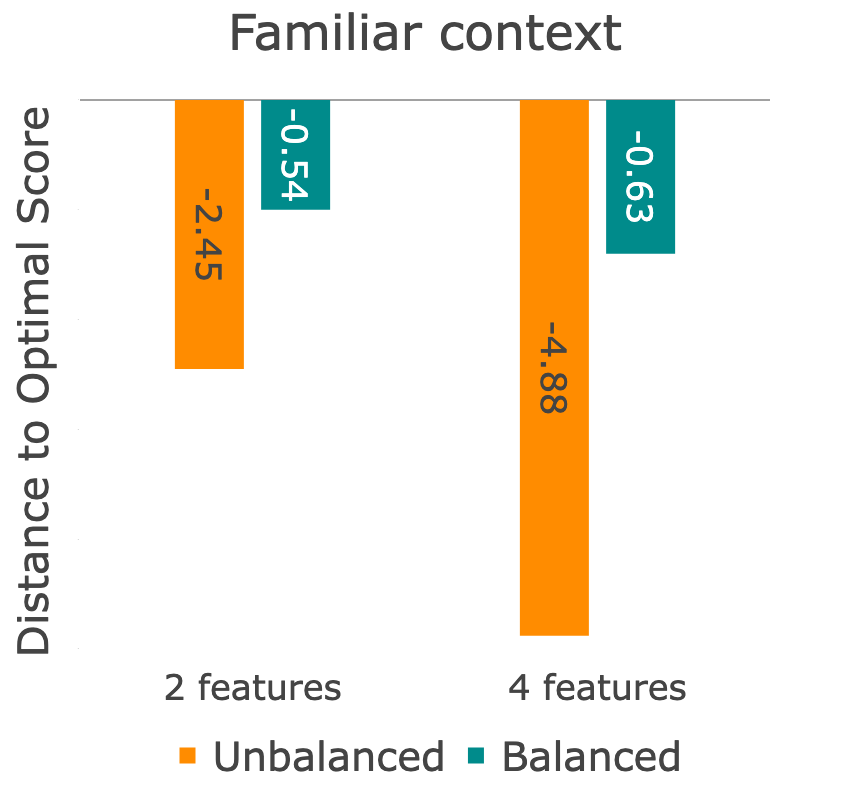
\includegraphics[width=0.2\textwidth]{Figures/distance_fam.png}
    \hspace{0.2in}
    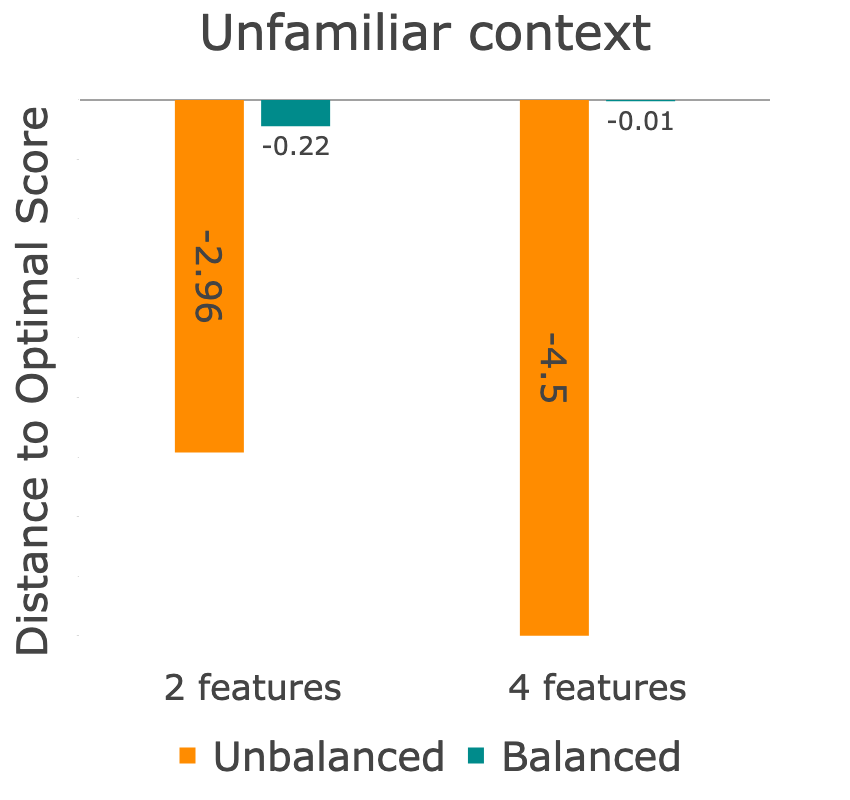
\includegraphics[width=0.2\textwidth]{Figures/distance_unf.png}
    \caption{The average distance to optimal ($\vtheta^T\vx_\text{NB}-\vtheta^T\vx_\text{B}$) for the four scenarios and two contexts.}
    \Description[Survey results showing the distance to optimal]{The average distance to optimal ($\vtheta^T\vx_\text{NB}-\vtheta^T\vx_\text{B}$) for the four scenarios.}
    \label{fig:dist-to-opt}
\end{figure}


In Figure~\ref{fig:dist-to-opt}, we observe that in the familiar context scenarios as the number of features increases, adding more complexity to the model, participants will move further away from the optimal score in balanced and unbalanced cases. The increase in the unbalanced case is almost double that of the balanced case. This indicates that we observe behavioral responses even in the balanced case, indicating biases beyond those in our theoretical predictions. For a fixed number of features, we see that answers are far from optimal when we have unbalanced features. Increasing the number of features will also lead to worse answers. On the other hand, in the unfamiliar context scenario we see the same pattern and numbers for unbalance features. However, with balanced features, the distance from optimal decreases compared to the familiar case. This could be a result of agents relying more on the model and the explanation when the context becomes unfamiliar and therefore respond more rationally. This does not necessarily mean that relying on the model in an unfamiliar context is better. Over reliance on AI models can also be problematic \cite{vasconcelos2023explanations, passi2022overreliance, buccinca2021trust}.

\begin{table}[ht]
    \caption{Number of responses in each scenario, (B) balanced and (U) unbalanced features for familiar context} 
    \label{table:number-of-responses-fam}
    \begin{center}
        \begin{tabular}{llll}
        \textbf{Scenario (familiar)}  &\textbf{Opt.} &\textbf{1-feature} &\textbf{Sub-opt.} \\
        \hline \\[-4.8pt]
        2-features (B) & 21 & 0 & 6 \\
        4-features (B) & 14 & 1 & 10 \\
        2-features (U) & 5 & 3 & 16 \\
        4-features (U) & 1 & 1 & 22
        \end{tabular}
    \end{center}
\end{table}

\begin{table}[ht]
    \caption{Number of responses in each scenario, (B) balanced and (U) unbalanced features for unfamiliar context} 
    \label{table:number-of-responses-unf}
    \begin{center}
        \begin{tabular}{llll}
        \textbf{Scenario (unfamiliar)}  &\textbf{Opt.} &\textbf{1-feature} &\textbf{Sub-opt.} \\
        \hline \\[-4.8pt]
        2-features (B) & 24 & 0 & 4 \\
        4-features (B) & 23 & 0 & 5 \\
        2-features (U) & 5 & 0 & 26 \\
        4-features (U) & 0 & 1 & 31
        \end{tabular}
    \end{center}
\end{table}

Table~\ref{table:number-of-responses-fam} shows that not only does the average distance from the optimal score increase with added complexity, but also the number of participants that responded sub-optimally increases. Most participants could find the optimal answers in the balanced cases, but most responded sub-optimally in the unbalanced cases. On the other hand, Table~\ref{table:number-of-responses-unf} indicates no significant difference in the number of people who responded sub-optimally to 2-feature and 4-feature conditions in the balanced case. However, we see The same pattern as in Table~\ref{table:number-of-responses-fam} for the unbalanced case.

\textbf{Participants exhibit different behavioral biases.} 
The unbalanced scenarios suggest that the behavior of most participants aligns with a Prelec function when (mis)perceiving feature importance. Specifically, the sub-optimal responses provided by the majority of participants would be considered optimal if the weights were adjusted according to Prelec function with $\gamma\le 0.64$ for two features scenario and $\gamma\le 0.55$ for four features scenario. This indicates that their decision-making may be systematically influenced by distorted perceptions of feature importance, consistent with the characteristics of the Prelec function. This leads them to under-invest in the most important feature and over-invest in the least important one. Participants not following the Prelec function tend to allocate all their budget to the most important feature.


The results from the balanced scenarios shed light on another behavioral bias: In the case of similar importance, participants invest more in the feature with a lower starting point (the resume in familiar context and VO2 max in the unfamiliar context). In the balanced scenarios, we notice that most participants respond without a behavioral bias, as predicted by the bias and Prelec functions. However, some participants responded sub-optimally, all over-investing in the feature with a lower starting point (resume or VO2 max). In the unbalanced four-feature case with familiar context, the average investment in the resume is higher despite the resume and the cover letter having the same importance, same statement is true for unfamiliar case and VO2 max and arterial stiffness index, indicating that this occurs for any two features with the same weight regardless of the importance of other features or the context. 

Focusing on the unbalanced scenarios, we see that the number of participants who respond with the optimal answer drops when we increase the number of features. More participants decide to invest all their budget in the most important feature. Findings from the unbalanced two-feature scenario show that if participants do not invest all their budget in the most important feature, they under-invest in it. 

\begin{table}[ht]
    \caption{Average distance of investment in most important and least important features in unbalanced scenarios from the optimal.}\label{table:avg-dist-from-opt}
    \begin{center}
        \begin{tabular}{lll}
         &\textbf{Most important} &\textbf{Least important} \\
        \hline \\[-4.8pt]
        2-features (Familiar) & -2.13 hours & +2.13 hours \\
        2-features (Unfamiliar) & -2.26 hours & +2.26 hours \\
        4-features (Familiar) & -4.11 hours & +1.76 hours \\
        4-features (Unfamiliar) & -3.90 hours & +1.64 hours
        \end{tabular}
    \end{center}
\end{table}
Assuming the Prelec function, we find that $\gamma$ for the participants answering the unbalanced two-features scenario is $\gamma \le 0.64$, vs. $\gamma\le 0.55$ for four-features. (The lower the $\gamma$ in the Prelec function, the more intense the bias.) These upper bounds come from the fact that participants must underestimate the importance of the most important feature enough so that they conclude it is better to invest in the second most important feature.  

Another interesting observation in the unbalanced four-features scenario is that, even though any investment in the least important feature was sub-optimal, 18 participants in the familiar context and 27 participants in the unfamiliar context still invested. This could be either a result of participants overestimating the importance of the least important feature, or a different behavioral bias, where participants prefer to invest in all options, and avoid leaving any feature as is. {A more detailed statistical report of the user study is included in Appendix~\ref{sec:app-stats-survey}}

\section{Conclusion}\label{sec:conclusion}
We presented a new strategic classification framework that accounts for the cognitive biases (in the form of probability weighing functions) of strategic agents when assessing feature importance. 
{Our hypothesis of humans' behavioral biases manifesting as weight misperceptions was motivated by commonly studied Prospect Theoretical models \cite{kahnemann1979prospect}, which found that individuals tend to overweigh or underweigh certain outcomes when making decisions under risk. While not directly a notion of risk, we hypothesized that these biases may also arise when feature importance weights are interpreted by users.}
{Given this type of behavioral bias,} we{, first theoretically, } identify conditions under which the agents over- or under-invest in different features, the impacts of this on a firm's choice of classifier, and the impacts on the firm's utility and agents' welfare. Then, through a user study, we provide support for our theoretical model and results, showing that most participants respond sub-optimally when provided with an explanation of feature importance/contribution, over-investing in the most important feature, while under-investing in the least important one, {a behavior explainable by our proposed weight misperceptions model}. {That said, we recognize that the study of behavioral biases in decision-making is a rich area, and exploring alternative forms of bias beyond weight or threshold misperception (in both theory and user studies) is an exciting avenue for future research; we hope our work provides a first step in this direction.}
Exploring analytical models accounting for biases beyond misperception of feature weights {such as misperception in the cost function (or alternative firm cost functions, or misalignment between users/firm's perception of others' costs) which would not only alter the underlying movement trajectory of each agent (Fig.~\ref{fig:2d-approx-illustration}) but would also affect the constraint $c(\vx,\vx_0)\le B$, complicates the analysis. More general costs such as non-distance-based costs}, and exploring the possibility of designing explanation methods that can help mitigate biases, are also important directions for further investigation. 




% \section{Rights Information}

% Authors of any work published by ACM will need to complete a rights
% form. Depending on the kind of work, and the rights management choice
% made by the author, this may be copyright transfer, permission,
% license, or an OA (open access) agreement.

% Regardless of the rights management choice, the author will receive a
% copy of the completed rights form once it has been submitted. This
% form contains \LaTeX\ commands that must be copied into the source
% document. When the document source is compiled, these commands and
% their parameters add formatted text to several areas of the final
% document:
% \begin{itemize}
% \item the ``ACM Reference Format'' text on the first page.
% \item the ``rights management'' text on the first page.
% \item the conference information in the page header(s).
% \end{itemize}

% Rights information is unique to the work; if you are preparing several
% works for an event, make sure to use the correct set of commands with
% each of the works.

% The ACM Reference Format text is required for all articles over one
% page in length, and is optional for one-page articles (abstracts).

% \section{CCS Concepts and User-Defined Keywords}

% Two elements of the ``acmart'' document class provide powerful
% taxonomic tools for you to help readers find your work in an online
% search.

% The ACM Computing Classification System ---
% \url{https://www.acm.org/publications/class-2012} --- is a set of
% classifiers and concepts that describe the computing
% discipline. Authors can select entries from this classification
% system, via \url{https://dl.acm.org/ccs/ccs.cfm}, and generate the
% commands to be included in the \LaTeX\ source.

% User-defined keywords are a comma-separated list of words and phrases
% of the authors' choosing, providing a more flexible way of describing
% the research being presented.

% CCS concepts and user-defined keywords are required for for all
% articles over two pages in length, and are optional for one- and
% two-page articles (or abstracts).




% \section{Citations and Bibliographies}

% The use of \BibTeX\ for the preparation and formatting of one's
% references is strongly recommended. Authors' names should be complete
% --- use full first names (``Donald E. Knuth'') not initials
% (``D. E. Knuth'') --- and the salient identifying features of a
% reference should be included: title, year, volume, number, pages,
% article DOI, etc.

% The bibliography is included in your source document with these two
% commands, placed just before the \verb|\end{document}| command:
% \begin{verbatim}
%   \bibliographystyle{ACM-Reference-Format}
%   \bibliography{bibfile}
% \end{verbatim}
% where ``\verb|bibfile|'' is the name, without the ``\verb|.bib|''
% suffix, of the \BibTeX\ file.

% Citations and references are numbered by default. A small number of
% ACM publications have citations and references formatted in the
% ``author year'' style; for these exceptions, please include this
% command in the {\bfseries preamble} (before the command
% ``\verb|\begin{document}|'') of your \LaTeX\ source:
% \begin{verbatim}
%   \citestyle{acmauthoryear}
% \end{verbatim}


%   Some examples.  A paginated journal article \cite{Abril07}, an
%   enumerated journal article \cite{Cohen07}, a reference to an entire
%   issue \cite{JCohen96}, a monograph (whole book) \cite{Kosiur01}, a
%   monograph/whole book in a series (see 2a in spec. document)
%   \cite{Harel79}, a divisible-book such as an anthology or compilation
%   \cite{Editor00} followed by the same example, however we only output
%   the series if the volume number is given \cite{Editor00a} (so
%   Editor00a's series should NOT be present since it has no vol. no.),
%   a chapter in a divisible book \cite{Spector90}, a chapter in a
%   divisible book in a series \cite{Douglass98}, a multi-volume work as
%   book \cite{Knuth97}, a couple of articles in a proceedings (of a
%   conference, symposium, workshop for example) (paginated proceedings
%   article) \cite{Andler79, Hagerup1993}, a proceedings article with
%   all possible elements \cite{Smith10}, an example of an enumerated
%   proceedings article \cite{VanGundy07}, an informally published work
%   \cite{Harel78}, a couple of preprints \cite{Bornmann2019,
%     AnzarootPBM14}, a doctoral dissertation \cite{Clarkson85}, a
%   master's thesis: \cite{anisi03}, an online document / world wide web
%   resource \cite{Thornburg01, Ablamowicz07, Poker06}, a video game
%   (Case 1) \cite{Obama08} and (Case 2) \cite{Novak03} and \cite{Lee05}
%   and (Case 3) a patent \cite{JoeScientist001}, work accepted for
%   publication \cite{rous08}, 'YYYYb'-test for prolific author
%   \cite{SaeediMEJ10} and \cite{SaeediJETC10}. Other cites might
%   contain 'duplicate' DOI and URLs (some SIAM articles)
%   \cite{Kirschmer:2010:AEI:1958016.1958018}. Boris / Barbara Beeton:
%   multi-volume works as books \cite{MR781536} and \cite{MR781537}. A
%   couple of citations with DOIs:
%   \cite{2004:ITE:1009386.1010128,Kirschmer:2010:AEI:1958016.1958018}. Online
%   citations: \cite{TUGInstmem, Thornburg01, CTANacmart}.
%   Artifacts: \cite{R} and \cite{UMassCitations}.

% \section{Acknowledgments}

% Identification of funding sources and other support, and thanks to
% individuals and groups that assisted in the research and the
% preparation of the work should be included in an acknowledgment
% section, which is placed just before the reference section in your
% document.

% This section has a special environment:
% \begin{verbatim}
%   \begin{acks}
%   ...
%   \end{acks}
% \end{verbatim}
% so that the information contained therein can be more easily collected
% during the article metadata extraction phase, and to ensure
% consistency in the spelling of the section heading.

% Authors should not prepare this section as a numbered or unnumbered {\verb|\section|}; please use the ``{\verb|acks|}'' environment.

% \section{Appendices}

% If your work needs an appendix, add it before the
% ``\verb|\end{document}|'' command at the conclusion of your source
% document.

% Start the appendix with the ``\verb|appendix|'' command:
% \begin{verbatim}
%   \appendix
% \end{verbatim}
% and note that in the appendix, sections are lettered, not
% numbered. This document has two appendices, demonstrating the section
% and subsection identification method.


\begin{acks}
This work was supported in part a UCSD Jacobs School of Engineering Early Career Faculty Development award, and by the NSF program on Fairness in AI in collaboration with Amazon under Award IIS-2040800. Any opinions, findings, and recommendations expressed in this material are those of the authors.
\end{acks}


% %%
% %% The next two lines define the bibliography style to be used, and
% %% the bibliography file.
\bibliographystyle{ACM-Reference-Format}
\bibliography{references_FAccT}


\clearpage

% %%
% %% If your work has an appendix, this is the place to put it.
% \newpage
\appendix
% \title{Supplementary Materials}
\section{Additional related work}\label{sec:app-lit-review}
\textbf{Iterpretable Machine Learning and Explainable AI:} The interpretability of machine learning models and explainable AI is receiving more attention as it becomes more necessary for firms in various fields of work to explain an AI decision-making assistant or understand the algorithm's process for that specific decision \cite{ALI2023101805, peeking2018adadi}. Many studies have focused on providing guidelines and new objectives for the algorithm to ensure interpretability, \cite{freitas2014position} discusses the interpretability issues for five specific classification models and more generic issues of interpretability. \cite{lakkaraju2016decisionsets} provides a multi-objective optimization problem and uses model interpretability as a goal of the learning algorithm, \cite{lundberg2017shap} and \cite{ribeiro2016lime} provide methods for posthoc explanations. \cite{adebayo2018sanity} provides a method to evaluate an explanation method for image data. Many other works have also conducted user studies for finding or evaluating the guidelines using measures such as satisfaction, understanding, trust, etc. \cite{poursabzi2021manipulating, kulesza2015principles, sixt2022do}. 

\textbf{Strategic Classification:} Explanations enable users to potentially respond \cite{Camacho2011manipulation} to an algorithm to improve, meaning that they change their features to change their actual qualification or cheat, meaning that they manipulate their features to game the algorithm. This topic is extensively discussed in works such as \cite{Perdomo2020performative, Hardt2016strategic, Liu2020disparateequilibria, bechavod2021gaming, Hu2019disparate}. However, these works assume complete information on the model parameters, which is not necessarily a correct assumption. \cite{cohen2024bayesian} explores the partial information released by the firm and discusses the firm's optimization problem and agents' best response. \cite{haghtalab2023calibratedstackelberggameslearning} introduced the calibrated Stackelberg games where the agent does not have direct access to the firm's action. This can also be implemented in our framework where the firm uses $\vtheta$ but announces $\vtheta'$, and agents respond to $\vw(\vtheta')$. Another line of work called actionable recourse suggests giving actionable responses to users alongside the model explanation could be beneficial and help the users have a better outcome \cite{karimi2022recoursesurvey}. \cite{ustun2019recourse} provides an integer programming toolkit and introduces actionable recourse in linear regression. \cite{karimi2021algorithmicrecourse} introduces algorithmic recourse that allows people to act rather than understand. \cite{harris2022bayesian} combines the algorithmic recourse with partial information and has a firm that provides actionable recourse and steers agents. They show that agents and the firm are never worse off in expectation in this setting. 
% \section{Warm Up: One-dimensional features}
Consider the one-dimensional case where the classifier can be expressed as $h(x, \theta) = 1$ if and only if $x\ge \theta$, with $x, \theta \in [0,1]$. Assume we have a $\theta_0$, the non-strategic threshold, and a $\theta^*_\text{NB}$, the strategic threshold when the firm assumes agents are non-behavioral. From \cite{Milli2019socialcost} we already know $\theta_0 < \theta^*_\text{NB}$. However, if the agents are behavioral, this will not be the optimal threshold since the firm can increase its utility by considering agents' behavioral biases. To illustrate why this happens, consider the following setting; we know for behavioral agents and one-dimensional feature space, two scenarios can happen: (i) $w(\theta) < \theta$ and (ii) $w(\theta) > \theta$. Additionally, assume the firm does not know that the agents are behavioral, i.e., announces $\theta^*_\text{NB}$. 

\begin{proposition}\label{prop:B-NB_1D}
    For a one dimensional classifier, if $w(\theta)<\theta$, then $\theta^*_\text{B} = \theta_0 < \theta^*_\text{NB}$.
\end{proposition}
\begin{proof}
For this case, if $\tau^*_\text{NB}$ is announced, behavioral agents will react to $w(\tau^*_\text{NB})<\tau^*_\text{NB}$, so the agents that are manipulating their features will not be successful in their goal. They will only exert a \emph{behavioral cost} without being rewarded. Therefore, since the inequality is strict, there exists a $\tau^*_\text{B} < \tau^*_\text{NB}$ that lets the firm choose more qualified agents without worrying about accepting the unqualified agents that are gaming the features, which results in $\mathcal{U}(h(x, \tau^*_\text{B}))> \mathcal{U}(h(x, \tau^*_\text{NB}))$. Moreover, this case reduces to the case of non-responding agents, and the firm choosing $\tau_0$ will be optimal; the only difference would be the behavioral cost of unqualified agents, i.e., $c(x_\text{B}, x)$. 

Meaning that for $x<w(\tau^*_\text{B})$ we can write $\sP(h(\bar x_\text{B}, \theta)=y)=\sP(h(x, \theta)=y)$ because the total number of individuals below the threshold remain the same even though the distribution has changed. For $x>w(\tau^*_\text{B})$ nothing will be different since no one needs to manipulate their feature, and the distribution will also be the same as before, so we can write $\tau^*_\text{B}=\tau_0$.
\end{proof}

In Proposition~\ref{prop:B-NB_1D}, we see that by noticing the behavioral bias of the agents, the firm can increase their utility to the maximum. By defining \emph{individual burden} and \emph{social burden} as defined in \cite{Milli2019socialcost}, $b_h(x) = \min_{h(\hat x) = 1}c(\hat x, x)$ and $\mathcal{B}_{+}(h) = \mathbb{E}[b_h(x)|Y=1]$, respectively, and knowing that social burden is monotonically increasing in $\theta$, using Proposition~\ref{prop:B-NB_1D}, we can see from that for $w(\theta)<\theta$, the firm considering the behavioral bias of agents results in both increasing the utility of the firm and lowering the social burden, i.e., $\mathcal{U}
_\text{S}(h(x, \theta_{\text{B}})) > \mathcal{U}
_\text{S}(h(x, \theta_{\text{NB}}))$ and $\mathcal{B}
_{+}(\theta^*_\text{NB}) > \mathcal{B}
_{+}(\theta^*_\text{B}) = \mathcal{B}
_{+}(\theta_0)$ at the cost of lowering the utility of the agents manipulating their features by $c(\bar x_\text{B}, x)$. 

However, things will not be as smooth when $w(\theta)>\theta$ since the firm must find the tipping point according to the trade-off between accepting unqualified and not accepting qualified agents. 

\paragraph{A trade-off:} For the case where $w(\theta) > \theta$, if $\theta^*_\text{NB}$ is announced, the agents will react to $w(\theta^*_\text{NB}) 
> \theta^*_\text{NB}$ and the agents gaming their feature will not only successfully classify as qualified, but they will also be able to pass the threshold strictly. This means that the firm will be accepting unqualified individuals that have $x= w(\theta^*_\text{NB}) >\theta^*_\text{NB}$. Note that these agents will not surpass $x= w(\theta^*_\text{NB})$ since they will not receive any rewards, which will only be more costly. 

For $\theta > \theta^*_\text{NB}$, the firm will be cutting down the number of agents who choose to manipulate ($U_\text{B}>0$) at the cost of losing truly qualified agents. And, for $\theta < \theta^*_\text{NB}$, the firm will gain utility by accepting more qualified agents. Still, it will have a loss on utility by automatically accepting more unqualified agents, plus an additional loss by having agents manipulate their feature. 

Therefore, $\theta^*_\text{B}$ will be where the utility gained from not accepting the unqualified agents who manipulate equals the utility loss of not accepting the truly qualified agents. While discussing the decision boundary, agents' response, and firms' strategic choice in one dimension is simple, we miss a few crucial points compared to higher dimensions. In higher dimensions, we can have a subset of agents that (1) will manipulate their features not making it to the threshold while they could if they were not biased, (2) will manipulate their features and, despite being biased, will pass the threshold, (3) will not manipulate their features but they would if they were not biased, and (4) will manipulate their features even though they are positively classified! These subsets of agents are of interest as we can understand and respond to the collective behavior of users by anticipating and discussing these subsets. 

% \section{Two Dimensional Features}
% In this section, we try to identify various subsets of agents that behave sub-optimally. We leave the discussion of the effects of these agents on the firm's utility and the firm's response for Section~\ref{sec:high-dim}. 

% In the case of an unlimited budget or high reward for positive classification compared to the cost ($r\ge c_{\max}$ where $c_{\max}=\max_{x', x}c(x',x)$), there is no ``optimal'' choice for the strategic firm as the classifier will end up accepting all the agents after manipulation, i.e., all agents with $\vtheta^T\vx_0 < \theta_0$ will be able to make it to $\vtheta^T\vx = \theta_0$ for any pair of $(\vtheta, \theta_0)$. However, the firm can analyze a trade-off if the agents are behavioral since not all the agents will be able to make it to the actual decision boundary. With a limited budget, the scenarios will be slightly different. 

% Let's begin by discussing a straightforward example in two dimensions. This example will serve as an introductory guide to the results we will explore by helping us better understand the underlying principles and how they apply in more complex scenarios: 
% \begin{example}\label{ex:simple-2D}
%     Consider a scenario where agents have two features, but only one is actionable, i.e., they can only manipulate one feature. Let this feature be $x_1$. This way, the agents' features after manipulation will look like ($x_1+\delta, x_2$). The optimal feature manipulation $\delta_\text{NB}$ is when $\theta_0 - \theta x_1 - (1-\theta)x_2 = \theta\delta_\text{NB}$, which, if agents are non-behavioral, they can successfully calculate and reach the threshold. However, behavioral agents will solve for a $\delta_\text{B}$ where $\theta_0 - w(\theta) x_1 - (1-w(\theta))x_2 = w(\theta)\delta_\text{B}$. Therefore, direct calculation shows that behavioral agents will over-invest ($\delta_\text{NB} < \delta_\text{B}$) when $x_2 < \theta_0$ and will under-invest ($\delta_\text{B} < \delta_\text{NB}$) when $x_2 > \theta_0$. 
% \end{example}

% In Example~\ref{ex:simple-2D}, we can identify the agents that under-invest or over-invest in their actionable feature, and the condition only depends on their non-actionable feature, and the intensity of bias will only change the amount of under/over-investment. However, when both features are actionable, agents can (1) under-invest in one and over-invest in the other, (2) under-invest in both, and (3) over-invest in both. 

\section{Alternative Cost Functions}\label{app:alternative_costs}

We next show that regions of differing responses between behavioral and non-behavioral agents, similar to those depicted in Figure~\ref{fig:highlighted}, will also emerge under quadratic and weighted Manhattan cost functions. We also describe the cost function presented to users' in our experiments, which can be viewed as an approximation of a quadratic cost.

\paragraph{Quadratic Cost Function.}
The following lemma characterizes the post-strategic features under the quadratic cost $c(\vx, \vx_0)=\sum_i c_i(x_{i}-x_{i,0})^2$.
\begin{lemma}\label{lemma:quad-cost-band}
    Let $\mC$ denote a diagonal matrix with $c_i$'s as its diagonal, and let $\vy$ denote the feature vectors satisfying $\vtheta^T\vy = \theta_0$. For an agent with starting feature vector $\vx_0$, if $\vx_0$ is in the n-dimensional ellipsoid determined by $B$ and $\mC$, i.e., if $(\vy-\vx_0)^T\mC (\vy-\vx_0)\le B$,
    \begin{align*}
        x_{\text{NB}, i} = \frac{\theta_{0}-\vtheta^T\vx_0}{\sum_j \frac{\theta_j^2}{c_j}}\cdot \frac{\theta_i}{c_i}+x_{0,i}~.
    \end{align*}
    Otherwise, $\vx_\text{NB}=\vx_0$. For behaviorally biased agents, $\vx_\text{B}$ is obtained similarly by replacing $\vtheta$ with $\vw(\vtheta)$.
\end{lemma}

Figure~\ref{fig:BR-illustration-quad-cost} illustrates the best-responses of Lemma~\ref{lemma:quad-cost-band} for rational (non-behavioral) and biased (behavioral) agents. Specifically, the condition in Lemma~\ref{lemma:quad-cost-band} constructs an $n$-dimensional ellipsoid around every point on the line $\vtheta^T\vx = \theta_{0}$, containing agents who have sufficient budget to strategically change their features to reach that particular point on the boundary, with the coefficients $c_i$ determining the scaling along each axis. %For $c_i=c, \forall i$, the ellipsoid becomes an n-dimensional sphere; for $c=1$, the cost becomes the norm-2 cost. 
Since the scaling of the ellipsoid does not depend on the point of the line we are focusing on, the union of these ellipsoids (determining the set of all agents who can afford to be classified positively through gaming) forms a band below the line $\vtheta^T\vx=\theta_0$. Note that this band differs from the one in Lemma~\ref{lemma:band-optimization}. 

\begin{figure}[ht]
    \centering
    \begin{subfigure}[t]{0.22\textwidth}
        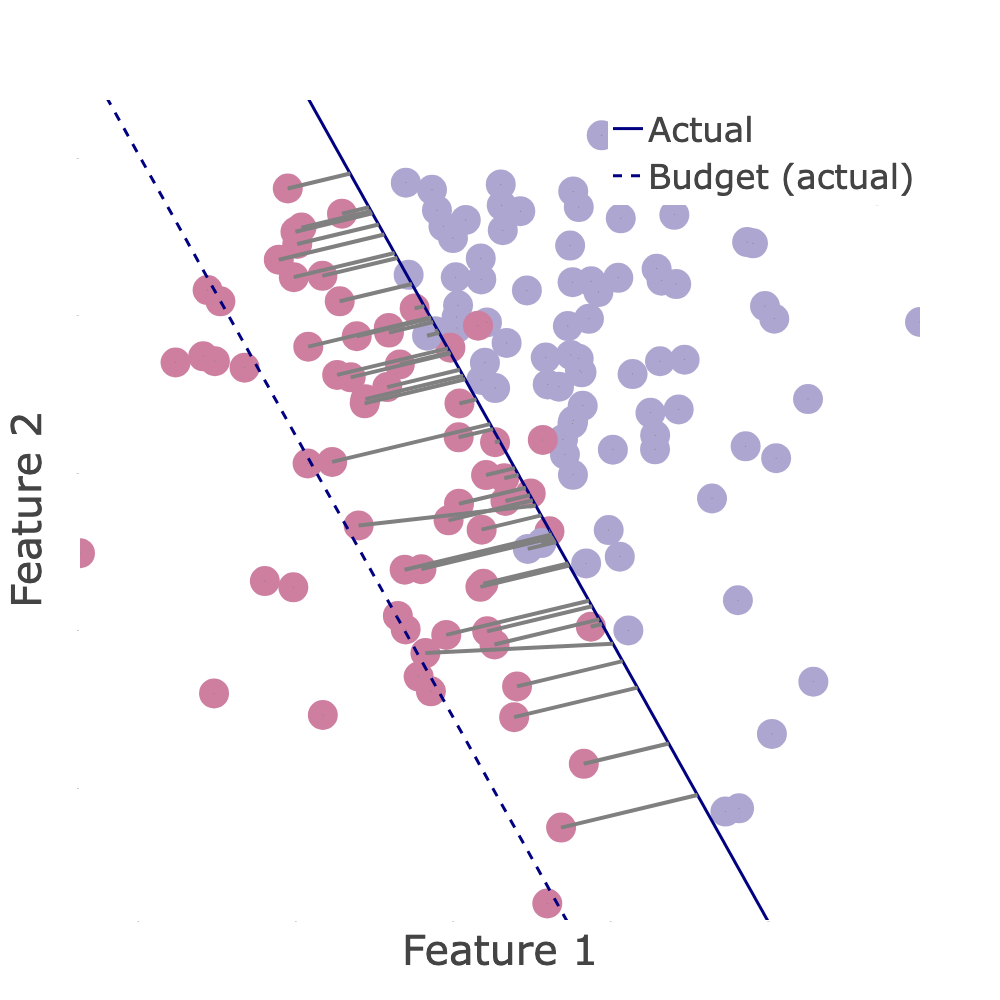
\includegraphics[width=0.9\textwidth]{Figures/quad-NB.png}
            \caption{Rational response}
            \Description[Rational response under quadratic cost]{This figure shows the rational response of agents to a known threshold classifier in 2 dimensions under quadratic cost.}
        \label{fig:NB-arrows-quad-cost}
    \end{subfigure}
    \hspace{0.01in}
    \begin{subfigure}[t]{0.22\textwidth}
        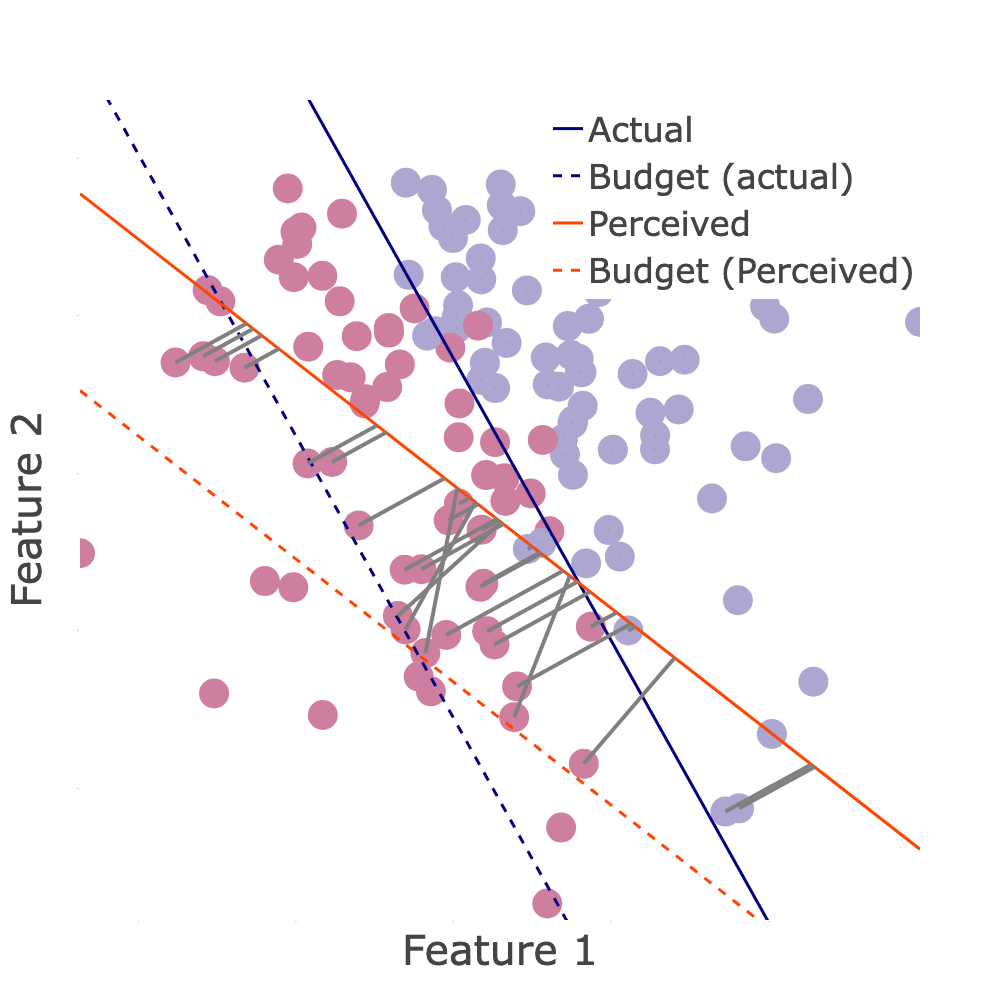
\includegraphics[width=0.9\textwidth]{Figures/quad-B.png}
        \caption{Biased response}
        \Description[Biased response under quadratic cost]{This figure shows the biased response of agents to a known threshold classifier in 2 dimensions under quadratic cost.}
        \label{fig:B-arrows-quad-cost}
    \end{subfigure}
    \caption{Strategic responses under quadratic costs.}
    \Description[Responses under quadratic cost]{This figure shows the responses of agents to a known threshold classifier in 2 dimensions under quadratic cost.}
    \label{fig:BR-illustration-quad-cost}
\end{figure} 

\paragraph{Weighted Manhattan Distance Cost Function.}
The following lemma characterizes the post-strategic features under the weighted Manhattan cost $c(\vx, \vx_0)=\sum_i c_i|x_{i}-x_{i,0}|$.
\begin{lemma}\label{lemma:manhattan-cost-band}
    Let $\ve_i$ be the unit vector with 1 in the $i$\textsuperscript{th} coordinate and 0 elsewhere, and $k = \arg\min_i \frac{c_i}{\theta_i}$. For an agent with starting feature $\vx_0$, if $\vtheta^T\vx_0 + \frac{\theta_k}{c_k}B \ge \theta_0$,
    \begin{align*}
        \vx_\text{NB} = \vx_0 + (\theta_0-\vtheta^T\vx_0)\frac{c_k}{\theta_k}\ve_k~.
    \end{align*}
    Otherwise, $\vx_\text{NB}=\vx_0$. For behaviorally biased agents, $\vx_\text{B}$ is obtained similarly by replacing $\vtheta$ with $\vw(\vtheta)$.
\end{lemma}

Figure~\ref{fig:BR-illustration-lin-cost} illustrates the best-responses of Lemma~\ref{lemma:manhattan-cost-band} for rational (non-behavioral) and biased (behavioral) agents.
Again, the set of agents who can afford to game the system to receive a positive classification, as identified in Lemma~\ref{lemma:manhattan-cost-band}, is a band below the classifier (but different from those of Lemmas~\ref{lemma:band-optimization} and \ref{lemma:quad-cost-band}). In particular, under this cost, agents spend all their budget on changing the feature with the most ``bang-for-the-buck'' $\frac{c_i}{\theta_i}$ (or perceived bang-for-the-buck $\frac{c_i}{w_i(\vtheta)}$). As seen in the two-dimensional illustration in Figure~\ref{fig:BR-illustration-lin-cost}, this means that while it is optimal for rational agents to invest only in feature 2, those with behavioral bias believe feature 1 has a better return, leading to a sub-optimal response by them. We also note that even though the movements of agents in the specified band are different from the movement for the norm-2 cost, the bands form the same regions of differing responses as in Figure~\ref{fig:BR-illustration}, where agents overshoot, undershoot, do nothing at all, or needlessly change their features, when they are behaviorally biased. 

\begin{figure}[ht]
    \centering
    \begin{subfigure}[t]{0.22\textwidth}
        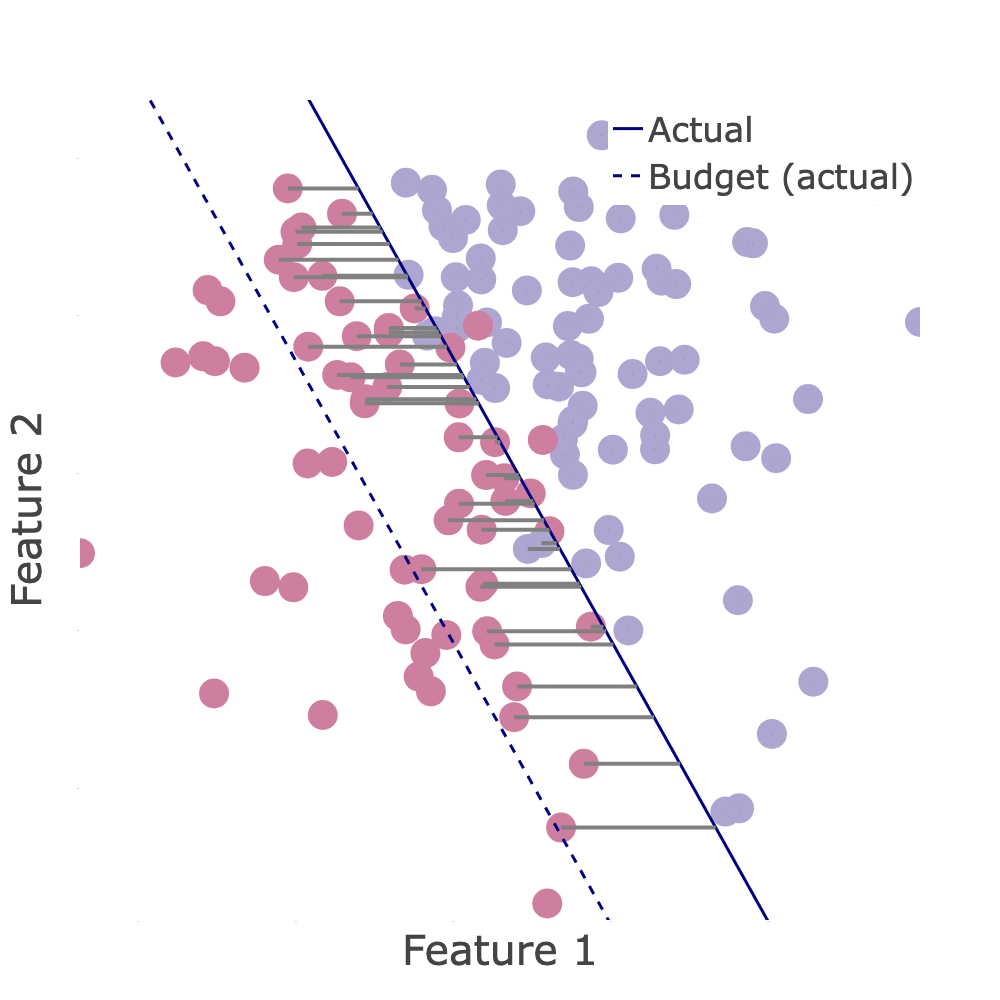
\includegraphics[width=0.9\textwidth]{Figures/lin-NB.png}
            \caption{Rational response}
            \Description[Rational response under Manhattan cost]{This figure shows the rational response of agents to a known threshold classifier in 2 dimensions under Manhattan cost.}
        \label{fig:NB-arrows-lin-cost}
    \end{subfigure}
    \hspace{0.01in}
    \begin{subfigure}[t]{0.22\textwidth}
        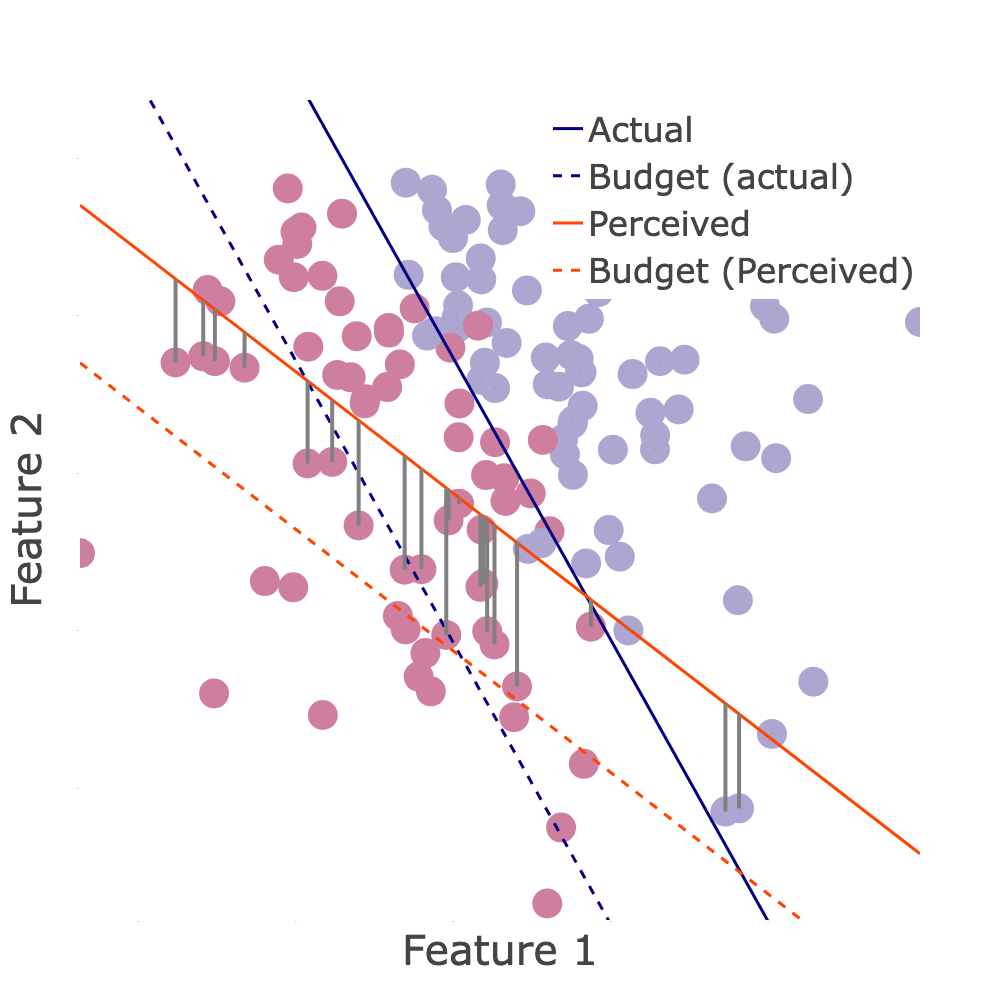
\includegraphics[width=0.9\textwidth]{Figures/lin-B.png}
        \caption{Biased response}
        \Description[Biased response under Manhattan cost]{This figure shows the biased response of agents to a known threshold classifier in 2 dimensions under Manhattan cost.}
        \label{fig:B-arrows-lin-cost}
    \end{subfigure}
    \caption{Strategic responses under Manhattan costs.}
    \Description[Responses under quadratic cost]{This figure shows the responses of agents to a known threshold classifier in 2 dimensions under Manhattan cost.}
    \label{fig:BR-illustration-lin-cost}
\end{figure}  

\paragraph{Cost Function in the User Studies.} For our human subject experiments in Section~\ref{sec:user-study}, to provide simple, yet actionable information to  participants, without the need for them to understand a specific form of cost function, we describe the cost of changing features to participants through a \emph{piecewise linear cost function}. This can be viewed as an approximation of a quadratic cost using a step function with a weighted Manhattan cost at each step, with the approximation improving as the number of steps increases (see the two-dimensional illustration in Figure~\ref{fig:2d-approx-illustration}). Specifically, in our user experiments, we break the budget $B$ into three steps of increments $B_1$, $B_2$, and $B_3$ with $B_1+B_2+B_3=B$, and assign a constant cost $c_1$, $c_2$, and $c_3$ for changing features at each increment. This means that in each step, agents face a weighted Manhattan cost, but overall, the cost is not fixed, and investing in a single feature is not optimal. 

\begin{figure}[ht]
    \centering
    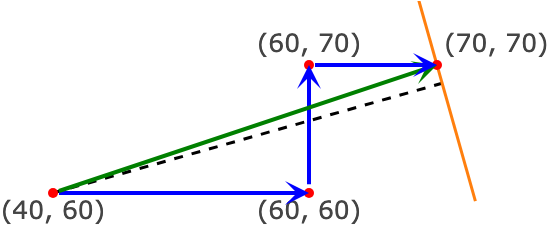
\includegraphics[width=0.8\linewidth]{Figures/illustration-single-movement.png}
    \caption{Strategic responses under a quadratic cost (green) vs. a piece-wise linear cost function (blue).}
    \Description[Responses under various costs]{This figure shows the responses of agents to a known threshold classifier in 2 dimensions under various costs with a numerical example.}
    \label{fig:2d-approx-illustration}
\end{figure}

\paragraph{More general cost functions.} We note that using more complex and general cost functions is possible. Specifically, the cost function impacts the movement trajectory of each point (agent), and while different cost functions might result in variations in the specific trajectories, the overall structure of the generic regions can remain unchanged; this is what we have observed with the $l_1$ and $l_2$ step costs functions. %For other $l_p$ norms with $p>1$ we see a different trajectory for each agent's movement but will again give us the same regions as in Figure~\ref{fig:highlighted}; the detailed analysis on cost functions is provided in Appendix~\ref{app:alternative_costs}.}

{Similarly, for $l_p$ norm cost functions we can see that the trajectory of an agent starting from $\vx_0$ is given by:
\begin{align}
    x_i = x_{0,i} - \frac{\vtheta^T\vx_0 - \theta_0}{\sum_i \frac{\theta_i^2}{|x_i-x_{0,i}^{p-2}|}}\times \frac{\theta_i}{|x_i-x_{0,i}^{p-2}|}~,
\end{align}
which will give us similar regions as shown in Figure~\ref{fig:highlighted}. That said, it is also not hard to find specific cost functions that might change the agents' trajectories in a way that alters the regions in Figure~\ref{fig:highlighted}. For instance, a fixed cost function $c(\vx,\vx_0) = c$, for all $\vx\neq\vx_0$, will allow the agents that can afford to manipulate their features to move to the decision boundary in whichever way they want. This can lead to expanding region 4 in Figure~\ref{fig:highlighted} to include regions 2 and 3. We view the analysis under such cost functions (those for which the 6 distinct regions in Figure~\ref{fig:highlighted} do not emerge) as a promising direction for future research.}
\section{Proofs}\label{sec:app-proofs}

\paragraph{Proof of Lemma~\ref{lemma:band-optimization}, Lemma~\ref{lemma:quad-cost-band}, and Lemma~\ref{lemma:manhattan-cost-band}}We show the NB case, the B case can be shown similarly. We divide the agents into two subsets: (1) Agents that will attempt to optimize and (2) agents that will not attempt to optimize. The first subset is the agents that will have a non-negative utility after optimization, i.e., will have $r-c(\vx_\text{NB}, \vx_0)$. For these agents, since their reward is constant, the optimization problem comes down to:
\begin{align}
    &\vx_\text{NB} := \argmax_\vx ~ r - c(\vx, \vx_0) \notag\\
    &\text{subject to}\quad \vtheta^T\vx = \theta_0
\end{align}
And the agents that are in the second subset will solve $\vx_\text{NB} := \argmin_\vx ~ c(\vx, \vx_0)$ which is simply $\vx_\text{NB}=\vx_0$.

\textbf{Lemma~\ref{lemma:band-optimization}:} For norm-2 cost we know this is the same as finding the closest point on a hyperplane to a given point. We know the solution for this problem is to move in the direction of the normal vector of the hyperplane by $d(\vx_0, \vtheta, \theta_0)=\frac{\theta_0-\vtheta^T\vx_0}{\norm{\vtheta}_2}$. This means that the solution for the agents in the first subset is $\vx_\text{NB} = \vx_0 + d(\vx_0, \vtheta, \theta_{0})\vtheta$.

\textbf{Lemma~\ref{lemma:quad-cost-band}} The quadratic cost is similar to norm-2 cost, by directly solving the optimization problem and having $\lambda$ to be the Lagrange multiplier for the constraint we find:
\begin{align}
    &x_{i, \text{NB}} = \frac{\lambda}{2}\frac{\theta_i}{c_i}+x_{i, 0} \text{ and } \notag\\
    &\frac{\lambda}{2} = \frac{\theta_0-\vtheta^T\vx_0}{\sum_j \frac{\theta_j^2}{c_j}}\Rightarrow x_{i, \text{NB}} = \frac{\theta_0-\vtheta^T\vx_0}{\sum_j\frac{\theta_j^2}{c_i}}\frac{\theta_i}{c_i}+x_{i, 0}
\end{align}
Which is, in some sense, a movement with a weighted distance from $\vx_0$ towards the hyperplane. 

\textbf{Lemma~\ref{lemma:manhattan-cost-band}} For the weighted Manhattan cost we are aiming to find the most efficient feature, i.e., the feature with the lowest $\frac{c_i}{\theta_i}$. 

\paragraph{Proof of Proposition~\ref{prop:under-invest-high-dim}}For a behavioral agent with $\vx_0$ that perceives $\theta_i$ as $\evw_i(\vtheta)$ to under-invest we need to have $\delta_i^{\text{B}}=d(\vx_0, \vw(\vtheta), \theta_0)\times \evw_i(\vtheta) < \delta_i^{\text{NB}}=d(\vx_0, \vtheta, \theta_0)\times \theta_i$, or $\frac{d(\vx_0, \vw(\vtheta), \theta_0)}{d(\vx_0, \vtheta, \theta_0)}<\frac{\theta_i}{\evw_i(\vtheta)}$. 

By knowing $\evw_i(\vtheta)<\theta_i$ then the agents with $d(\vx_0, \vw(\vtheta), \theta_0)\le d(\vx_0, \vtheta, \theta_0)$ will satisfy the condition since $\frac{d(\vx_0, \vw(\vtheta), \theta_0)}{d(\vx_0, \vtheta, \theta_0)}\le 1 < \frac{\theta_i}{\evw_i(\vtheta)}$ and under-invest in feature $i$. We can show the second statement similarly. 

The third statement of the proposition is a scenario where $\evw_1(\theta)<\theta_1$ where $\theta_1\ge \theta_i$ for all $i$, and we want to identify agents that will over-invest in that feature, i.e., $\frac{d(\vx_0, \vw(\vtheta), \theta_0)}{d(\vx_0, \vtheta, \theta_0)}>\frac{\theta_1}{\evw_1(\vtheta)}$. 

Since for the most important feature we have $\evw_1(\vtheta)=p(\theta_1)$, we can easily find the maximum of $\frac{\theta_1}{\evw_1(\vtheta)}$ for a given $\gamma$ by taking the derivative and using the function in \cite{Prelec1998}. This maximum occurs at $\theta^* = e^{-(\frac{1}{\gamma})^\frac{1}{\gamma-1}}$ meaning, $\frac{\theta_1}{\evw_1(\vtheta)}\le \frac{\theta^*}{\evw(\theta^*)} = \exp((\frac{1}{\gamma})^\frac{\gamma}{\gamma-1}-(\frac{1}{\gamma})^\frac{1}{\gamma-1})$. Therefore, using the same reasoning for the first two statements, agents with $\frac{d(\vx_0, \vw(\vtheta), \theta_0)}{d(\vx_0, \vtheta, \theta_0)}\ge \exp((\frac{1}{\gamma})^\frac{\gamma}{\gamma-1}-(\frac{1}{\gamma})^\frac{1}{\gamma-1})$ will over-invest in the most important feature, i.e., feature 1. {We can further write $\frac{d(\boldsymbol{x}_0, \boldsymbol{w}(\boldsymbol{\theta}), \theta_0)}{d(\boldsymbol{x}_0, \boldsymbol{\theta}, \theta_0)}\ge \exp((\frac{1}{\gamma})^\frac{\gamma}{\gamma-1}-(\frac{1}{\gamma})^\frac{1}{\gamma-1}) = \exp(\gamma^{-\frac{\gamma}{\gamma-1}}-\gamma^{-\frac{1}{\gamma-1}}) = \exp(\gamma^{\frac{\gamma}{1-\gamma}}-\gamma^{\frac{1}{1-\gamma}})$ which brings us to the expression in Proposition~\ref{prop:under-invest-high-dim}.}

\paragraph{Proof of Proposition~\ref{prop:mismatch-actual-b}}
We start the proof from the leftmost inequality in \eqref{eq:firm-loss-comp-benefit}. By the definition of $(\vtheta_\text{B}, \vtheta_{0, \text{B}})$ we can write 
\begin{align*}
    \E_{\vx\sim\mathcal{D}(\vw(\vtheta_\text{B}), \theta_{0, \text{B}})}[l(\vx, (\vtheta_\text{B}, \vtheta_{0, \text{B}}))]\le \E_{\vx\sim\mathcal{D}(\vw(\vtheta), \theta_{0})}[l(\vx, (\vtheta, \vtheta_0))    
\end{align*}
for all $(\vtheta, \vtheta_0)\neq (\vtheta_\text{B}, \vtheta_{0, \text{B}})$, i.e.,
\begin{align*}
    \sL((\vw(\vtheta_\text{B}), \theta_{0, \text{B}}), (\vtheta_\text{B}, \vtheta_{0, \text{B}}))\le \sL((\vw(\vtheta_\text{NB}), \theta_{0, \text{NB}}), (\vtheta_\text{NB}, \theta_{0, \text{NB}}))
\end{align*}
is always true. 

We next provide a characterization of the set of agents who fall within regions \framebox(7,9){1} and \framebox(7,9){3} in Figure~\ref{fig:highlighted}. These are the set of agents who will still pass the (true) decision boundary regardless of their biases. 
\begin{lemma}\label{lemma:H}
     For a given $(\vtheta, \theta_0)$, agents that satisfy $(1-\sigma(\vtheta))\theta_0\le(\vtheta-\sigma(\vtheta)\vw(\vtheta))^T\vx$, if given enough budget, will be accepted by the classifier, where $\sigma(\vtheta) \coloneqq \frac{\vtheta^T\vw(\vtheta)}{\norm{\vw(\vtheta)}^2}$ is a measure of the intensity of behavioral bias. 
\end{lemma}
\begin{proof}
    We can write agents' behavioral response as $\vx+\Delta_\text{B}$ with $\Delta_\text{B}=\frac{\theta_0-\vw(\vtheta)^T\vx}{\norm{\vw(\vtheta)}^2}\vw(\vtheta)$ for a given $(\vtheta, \theta_0)$. Agents that will have successful manipulation are the ones satisfying $\theta_0\le \vtheta^T(\vx+\Delta_\text{B})$ which, by substituting $\Delta_\text{B}$, can be written as:
\begin{align}
    &\vtheta_0\le \frac{\theta_0-\vw(\vtheta)^T\vx}{\norm{\vw(\vtheta)}^2}\vtheta^T\vw(\vtheta)+\vtheta^T\vx = \frac{\vtheta^T\vw(\vtheta)}{\norm{\vw(\vtheta)}^2}\theta_0+\notag\\
    &\bigg( \vtheta - \frac{\vtheta^T\vw(\vtheta)}{\norm{\vw(\vtheta)}^2} \vw(\vtheta) \bigg)^T \vx \Rightarrow(1-\sigma(\vtheta))\theta_0 \le (\vtheta-\sigma(\vtheta)\vw(\vtheta))^T\vx
\end{align}
    Where we defined $\sigma(\vtheta)\coloneqq\frac{\vtheta^T\vw(\vtheta)}{\norm{\vw(\vtheta}^2}$.
\end{proof}


To compare the firm's loss after biased and non-biased responses, we can break the feature space into the following regions ($\1(\cdot)$ is the indicator function):
\begin{enumerate}[label=\large\protect\textcircled{\small\arabic*}]
    \item $\1(\vtheta_\text{NB}^T\vx\ge\theta_{0, \text{NB}})$
    \item $\1(\vtheta_\text{NB}^T\vx\le\theta_{0, \text{NB}}-B)$
    \item $\1(\theta_{0, \text{NB}}-B\le\vtheta_\text{NB}^T\vx\le\theta_{0, \text{NB}})\1(\theta_{0, \text{NB}}-B\le\vw(\vtheta_\text{NB})^T\vx\le\theta_{0, \text{NB}}) \equiv \sA(\vtheta_\text{NB}, \theta_{0, \text{NB}})\cap \sA(\vw(\vtheta_\text{NB}), \theta_{0, \text{NB}})$
    \item $\1(\theta_{0, \text{NB}}-B\le\vtheta_\text{NB}^T\vx\le\theta_{0, \text{NB}})\1(\vw(\vtheta_\text{NB})^T\vx\ge\theta_{0, \text{NB}})$
    \item $\1(\theta_{0, \text{NB}}-B\le\vtheta_\text{NB}^T\vx\le\theta_{0, \text{NB}})\1(\vw(\vtheta_\text{NB})^T\vx\le\theta_{0, \text{NB}}-B)$
\end{enumerate}

We know that for $\vx\in {\Circled{1}}$ and $\vx\in\Circled{2}$, the expected loss for both response scenarios is the same since the agents in the two regions are either already qualified or will never make it to the decision boundary. Therefore, to compare the expected loss for two scenarios we would need to look at the differences in the rest of the regions. 

For $\vx\in\Circled{4}$ and $\vx\in\Circled{5}$ and biased responses, the expected loss would be the same as the non-strategic case. For $\vx\in\Circled{4}$ and $\vx\in\Circled{5}$ and the non-biased case, it could be higher or lower. For $\vx\in\Circled{3}$, the firm will have a lower (resp. higher) expected loss in the biased responses scenario if the truly unqualified agents are (resp. not) more than truly qualified agents. We furthermore focus on a subset of the region $\Circled{3}$ identified by Lemma~\ref{lemma:H}, region $\Circled{3a}$, which is the biased agents that will pass the threshold despite being biased. If we define the region identified by Lemma~\ref{lemma:H} by $\mathcal{H}(\vtheta_\text{NB}, \theta_{0, \text{NB}})$, then region $\Circled{3a}$ will be $\sA(\vtheta_\text{NB}, \theta_{0, \text{NB}})\cap \sA(\vw(\vtheta_\text{NB}), \theta_{0, \text{NB}}) \cap\mathcal{H}(\vtheta_\text{NB}, \theta_{0, \text{NB}})$. 

For a setting where the loss function rewards true positives and penalizes false positives as $-u^+ TP + u^- FP$, as higher loss is worse as we defined, we can write the following:
\begin{align}\label{eq:regions_NB}
    &\sL(\vtheta_\text{NB}, (\vtheta_\text{NB}, \theta_{0, \text{NB}}))=\mL_{\Circled{1}\cup\Circled{2}} + \notag\\
    &\int_{\vx\in\Circled{3}\cup\Circled{4}\cup\Circled{5}} \hspace{-0.9cm} \big( -u^+ p(\hat{y}=1 | \vx, y)f_1(\vx)\alpha_1 + u^- p(\hat{y}=1 | \vx, y)f_0(\vx)\alpha_0 \big) d\vx \\
    &\sL(\vw(\vtheta_\text{NB}), (\vtheta_\text{NB}, \theta_{0, \text{NB}}))=\mL_{\Circled{1}\cup\Circled{2}} + \notag\\
    &\int_{\vx\in\Circled{3a}} \big( -u^+ p(\hat{y}=1 | \vx, y)f_1(\vx)\alpha_1 + u^- p(\hat{y}=1 | \vx, y)f_0(\vx)\alpha_0 \big ) d\vx\label{eq:regions_B}
\end{align}

Where $\mL_{\Circled{1}\cup\Circled{2}}$ is the loss coming from regions $\Circled{1}$ and $\Circled{2}$ which is present in both scenarios. For $\sL(\vtheta_\text{NB}, (\vtheta_\text{NB}, \theta_{0, \text{NB}}))$, we know all the agents in $\Circled{3}\cup\Circled{4}\cup\Circled{5}$ will be accepted, i.e., $p(\hat{y}=1 | \vx\in\Circled{3}\cup\Circled{4}\cup\Circled{5}, y)=1$. Similar for $\sL(\vw(\vtheta_\text{NB}), (\vtheta_\text{NB}, \theta_{0, \text{NB}}))$ and $\vx\in\Circled{3a}$. 

We can see from \eqref{eq:regions_NB} and \eqref{eq:regions_B} that depending on the density of label 0 and label 1 agents in the region $\Circled{3a}$ and comparing it to the region $\Circled{3}\cup\Circled{4}\cup\Circled{5}$ we can have both $\sL(\vw(\vtheta_\text{NB}), (\vtheta_\text{NB}, \theta_{0, \text{NB}}))\le \sL(\vtheta_\text{NB}, (\vtheta_\text{NB}, \theta_{0, \text{NB}}))$ and $\sL(\vtheta_\text{NB},$ $(\vtheta_\text{NB}, \theta_{0, \text{NB}}))\le \sL(\vw(\vtheta_\text{NB}), (\vtheta_\text{NB}, \theta_{0, \text{NB}}))$ occur. The difference in expected loss lies in the region $\Circled{3}\cup\Circled{4}\cup\Circled{5}-\Circled{3a}$, or equivalently $\sS(\vtheta_\text{NB}, \theta_{0, \text{NB}}) \coloneqq \sA(\vtheta_\text{NB}, \theta_{0, \text{NB}})/(\sA(\vtheta_\text{NB}, \theta_{0, \text{NB}})\cap \sA(\vw(\vtheta_\text{NB}), \theta_{0, \text{NB}}) \cap\mathcal{H}(\vtheta_\text{NB}, \theta_{0, \text{NB}}))$, we can write the following for $\sL(\vtheta_\text{NB}, (\vtheta_\text{NB}, \theta_{0, \text{NB}})) - \sL(\vw(\vtheta_\text{NB}), (\vtheta_\text{NB}, \theta_{0, \text{NB}}))\le 0$ (resp. $\ge 0$):
\begin{align}
    \int_{\vx\in\sS(\vtheta_\text{NB}, \theta_{0, \text{NB}})}(-u^+f_1(\vx)\alpha_1+u^-f_0(\vx)\alpha_0)dx \le 0 \text{ (resp. $\ge$ 0)}
\end{align}

Therefore, if the density of unqualified agents is higher (resp.~lower) than the density of qualified agents over the region $\sA(\vtheta_\text{NB}, \theta_{0, \text{NB}})/$ $(\sA(\vtheta_\text{NB}, \theta_{0, \text{NB}})\cap \sA(\vw(\vtheta_\text{NB}), \theta_{0, \text{NB}}) \cap\mathcal{H}(\vtheta_\text{NB}, \theta_{0, \text{NB}}))$, then:
\begin{align*}
    &\sL(\vw(\vtheta_\text{NB}), (\vtheta_\text{NB}, \theta_{0, \text{NB}}))\le \sL(\vtheta_\text{NB}, (\vtheta_\text{NB}, \theta_{0, \text{NB}})) \notag\\
    &(\text{resp. } \sL(\vtheta_\text{NB}, (\vtheta_\text{NB}, \theta_{0, \text{NB}}))\le \sL(\vw(\vtheta_\text{NB}), (\vtheta_\text{NB}, \theta_{0, \text{NB}})))
\end{align*}

To show the last statement of the proposition, we need to compare $\sL(\vw(\vtheta_\text{NB}), (\vtheta_\text{NB}, \theta_{0, \text{NB}}))$ and $\sL(\vw(\vtheta_\text{B}), (\vtheta_\text{B}, \theta_{0, \text{B}})))$ directly. The difference between these two losses comes from the region where agents will be accepted by $(\vtheta_\text{NB}, \theta_{0, \text{NB}})$ and not by $(\vtheta_\text{B}, \theta_{0, \text{B}})$, and vice versa, after agents' response. Mathematically, for agents responding to $(\vtheta_\text{NB}, \theta_{0, \text{NB}})$ without bias, we can show the agents accepted by $(\vtheta_\text{NB}, \theta_{0, \text{NB}})$ by $\sY(\vtheta_\text{NB}, \theta_{0,\text{NB}})\cup \sA(\vtheta_\text{NB}, \theta_{0,\text{NB}})$. We want the intersection of this set with the agents not accepted by $(\vtheta_\text{B}, \theta_{0, \text{B}})$, which brings us to $\sT_1=(\sY(\vtheta_\text{NB}, \theta_{0,\text{NB}})\cup \sA(\vtheta_\text{NB}, \theta_{0,\text{NB}}))\cap \sN(\vtheta_\text{B}, \theta_{0,\text{B}})$. 

Similarly, for agents responding to $(\vtheta_\text{NB}, \theta_{0, \text{NB}})$ with bias, we can show the agents accepted by $(\vtheta_\text{B}, \theta_{0, \text{B}})$ and not by $(\vtheta_\text{NB}, \theta_{0, \text{NB}})$ by $(\sY(\vtheta_\text{B}, \theta_{0,\text{B}}) \cap \sN(\vtheta_\text{NB}, \theta_{0,\text{NB}}))/\sA(\vtheta_\text{NB}, \theta_{0,\text{NB}})$. However, in this scenario, we need to also account for agents that make it past the actual decision boundary despite being behavioral, i.e., agents in the region $\mathcal{H}(\vtheta_\text{B}, \theta_{0,\text{B}})\cap \sA(\vw(\vtheta_\text{B}), \theta_{0,\text{B}})$, bringing us to $\sT_2 = (\mathcal{H}(\vtheta_\text{B}, \theta_{0,\text{B}})\cap \sA(\vw(\vtheta_\text{B}), \theta_{0,\text{B}}))\cup ( (\sY(\vtheta_\text{B}, \theta_{0,\text{B}}) \cap \sN(\vtheta_\text{NB}, \theta_{0,\text{NB}}))/\sA(\vtheta_\text{NB}, \theta_{0,\text{NB}}) )$. 

We need the total loss from region $\sT_1$ to be lower than the total loss from the region $\sT_2$ in the two scenarios for $\sL(\vtheta_\text{NB}, (\vtheta_\text{NB}, \theta_{0, \text{NB}}))\le \sL(\vw(\vtheta_\text{B}), (\vtheta_\text{B}, \theta_{0, \text{B}}))$ to be true. Meaning that we need $\int_{\vx\in\sT_1}(-u^+$ $f_1(\vx)\alpha_1+u^-f_0(\vx)\alpha_0)d\vx \le \int_{\vx\in\sT_2}(-u^+f_1(\vx)\alpha_1+u^-f_0(\vx)\alpha_0)d\vx$ to be true for $\sL(\vtheta_\text{NB}, (\vtheta_\text{NB}, \theta_{0, \text{NB}}))\le \sL(\vw(\vtheta_\text{B}), (\vtheta_\text{B}, \theta_{0, \text{B}}))$, and the last inequality of the statement comes from the optimality condition. 
% \section{Special Case: Two Dimensions}\label{sec:special2D}
Consider a two-dimensional feature space where, without loss of generality, feature 1 has a higher weight than feature 2, and agents manipulate their features to move to the nearest point on the (perceived) decision boundary. The agents that will under-invest in the first feature ($\delta_{1_\text{B}}<\delta_{1_\text{NB}}$) will be the ones who satisfy:
 \begin{align}\label{eq:underinvest1}
     \big( \frac{\theta^2}{\norm{\vtheta}_2^2} - \frac{w(\theta)^2}{\norm{\vw(\vtheta)}_2^2} \big)x_1 + \big( \frac{\theta(1-\theta)}{\norm{\vtheta}_2^2} - \frac{w(\theta)(1-w(\theta))}{\norm{\vw(\vtheta)}_2^2} \big)x_2 < \big(\frac{w(\theta)}{\norm{\vw(\vtheta)}_2^2} - \frac{\theta}{\norm{\vtheta}_2^2} \big)\theta_0
 \end{align}
 and the agents who under-invest in the second feature ($\delta_{2_\text{B}}<\delta_{2_\text{NB}}$) will satisfy:
 \begin{align}\label{eq:underinvest2}
     \big( \frac{\theta(1-\theta)}{\norm{\vtheta}_2^2} - \frac{w(\theta)(1-w(\theta))}{\norm{\vw(\vtheta)}_2^2} \big)x_1 + \big( \frac{(1-\theta)^2}{\norm{\vtheta}_2^2} - \frac{(1-w(\theta))^2}{\norm{\vw(\vtheta)}_2^2} \big)x_2 < \big(\frac{1-w(\theta)}{\norm{\vw(\vtheta)}_2^2} - \frac{1-\theta}{\norm{\vtheta}_2^2} \big)\theta_0
 \end{align}
For agents that under-invest in only one of the features, we need one of the \eqref{eq:underinvest1} and \eqref{eq:underinvest2} to be true while the other is not. We rearrange \eqref{eq:underinvest1} and \eqref{eq:underinvest2} to get:
\begin{align}
    \textit{For under-investment in feature 1: }&\alpha x_1 + \beta x_2 < \tau\\
    \textit{For under-investment in feature 2: }&\alpha x_1 + \beta x_2 - (\bar\alpha x_1 + \bar\beta x_2 - \bar\tau) > \tau
\end{align}
Where:
\begin{align}
    &\alpha = \frac{\theta^2}{\norm{\vtheta}_2^2} - \frac{w(\theta)^2}{\norm{\vw(\vtheta)}_2^2}\quad,\quad \beta = \frac{(1-\theta)^2}{\norm{\vtheta}_2^2} - \frac{(1-w(\theta))^2}{\norm{\vw(\vtheta)}_2^2}\quad,\quad \tau = \big(\frac{w(\theta)}{\norm{\vw(\vtheta)}_2^2} - \frac{\theta}{\norm{\vtheta}_2^2} \big)\theta_0 \notag\\
    &\bar\alpha = \frac{\theta}{\norm{\vtheta}_2^2} - \frac{w(\theta)}{\norm{\vw(\vtheta)}_2^2}\quad,\quad \bar\beta = \frac{1-\theta}{\norm{\vtheta}_2^2} - \frac{1-w(\theta)}{\norm{\vw(\vtheta)}_2^2}\quad,\quad \bar\tau = \big(\frac{1}{\norm{\vw(\vtheta)}_2^2} - \frac{1}{\norm{\vtheta}_2^2} \big)\theta_0\notag
\end{align}
By defining $\xi \coloneqq \bar\alpha x_1 + \bar\beta x_2 - \bar\tau$ we can condition on the sign of $\xi$. By using $\xi$ we can say that biased agents:
\begin{enumerate}
    \item Will not under-invest in feature 1 (2) if they under-invest in feature 2 (1) and have $\xi > 0$.
    \item Under-investment (over-investment) in both features is only possible for agents with $\xi < 0$ ($\xi > 0$).
\end{enumerate}
Where:
\begin{align}\label{eq:xi}
    \xi = \big( \frac{\theta}{\norm{\vtheta}_2^2} - \frac{w(\theta)}{\norm{\vw(\vtheta)}_2^2} \big) x_1 + \big( \frac{1-\theta}{\norm{\vtheta}_2^2} - \frac{1-w(\theta)}{\norm{\vw(\vtheta)}_2^2} \big) x_2 - \big( \frac{1}{\norm{\vtheta}_2^2} - \frac{1}{\norm{\vw(\vtheta)}_2^2} \big) \theta_0
\end{align}

Using Proposition~\ref{prop:under-invest-high-dim}, a firm can use $\xi$ as a possible cost or benefit function for their algorithm to, for instance, steer individuals to over-invest in a feature that benefits them more or help them invest less in a feature with a high cost that they have been over-investing in as a result of their bias. After a closer look, \eqref{eq:xi} is the difference between line equations of actual decision boundary and perceived decision boundary.

The following special case illustrates how the agents' behavioral bias will make them under-invest or over-invest in some features in a more straightforward setting:

Consider a setting with two actionable features. We consider a case where $\norm{\vtheta}_2 = \norm{\vw(\vtheta)}_2$. This situation can occur if we look at $\vw(\vtheta)$ as a rotation transform of $\vtheta$. Furthermore, if we consider the function introduced by \cite{Prelec1998}, then for $w(\theta)<\theta$ and in two dimensions, this occurs once for each $\gamma$. This is possible because in two dimensions we can write $\theta>1-\theta$ without loss of generality and by using the function in \cite{Prelec1998} we know that for larger $\theta$ we have $w(\theta)<\theta$. We can write:
\begin{itemize}
    \item Agents that under-invest in feature 1 ($\delta_{1_\text{B}}<\delta_{1_\text{NB}}$):
    \begin{align}\label{eq:example_underinvest_1}
         (\theta+w(\theta))x_1 - (\theta+w(\theta)-1)x_2 < \theta_0
    \end{align}
    \item Agents that under-invest in feature 2 ($\delta_{2_\text{B}}<\delta_{2_\text{NB}}$):
    \begin{align}\label{eq:example_underinvest_2}
         (\theta+w(\theta))x_1 - (\theta+w(\theta)-1)x_2 - (x_1-x_2) > \theta_0
    \end{align}
\end{itemize}
By looking at \eqref{eq:example_underinvest_1} and \eqref{eq:example_underinvest_2} we can identify a few interesting subsets of agents:
\begin{itemize}
    \item Agents that under-invest in feature 1 (2) and have $x_1\ge x_2$ will over-invest in feature 2 (1). Similarly, agents that under-invest in feature 2 (1) and have $x_1\ge x_2$ will over-invest in feature 1 (2).
    \item Agents that optimally invest in feature 1 and have $x_1<x_2$ ($x_1>x_2$) will under-invest (over-invest) in feature 2. Similarly, agents that optimally invest in feature 2 and have $x_1 < x_2$ ($x_1>x_2$) will under-invest (over-invest) in feature 1. 
    \item Agents that optimally invest in feature 2 and have $x_1=x_2$ will also invest in feature 1 optimally. 
    \item Agents that under-invest in both features will have $x_1<x_2$ and agents that over-invest in both features will have $x_1>x_2$.
\begin{figure}
    \centering
    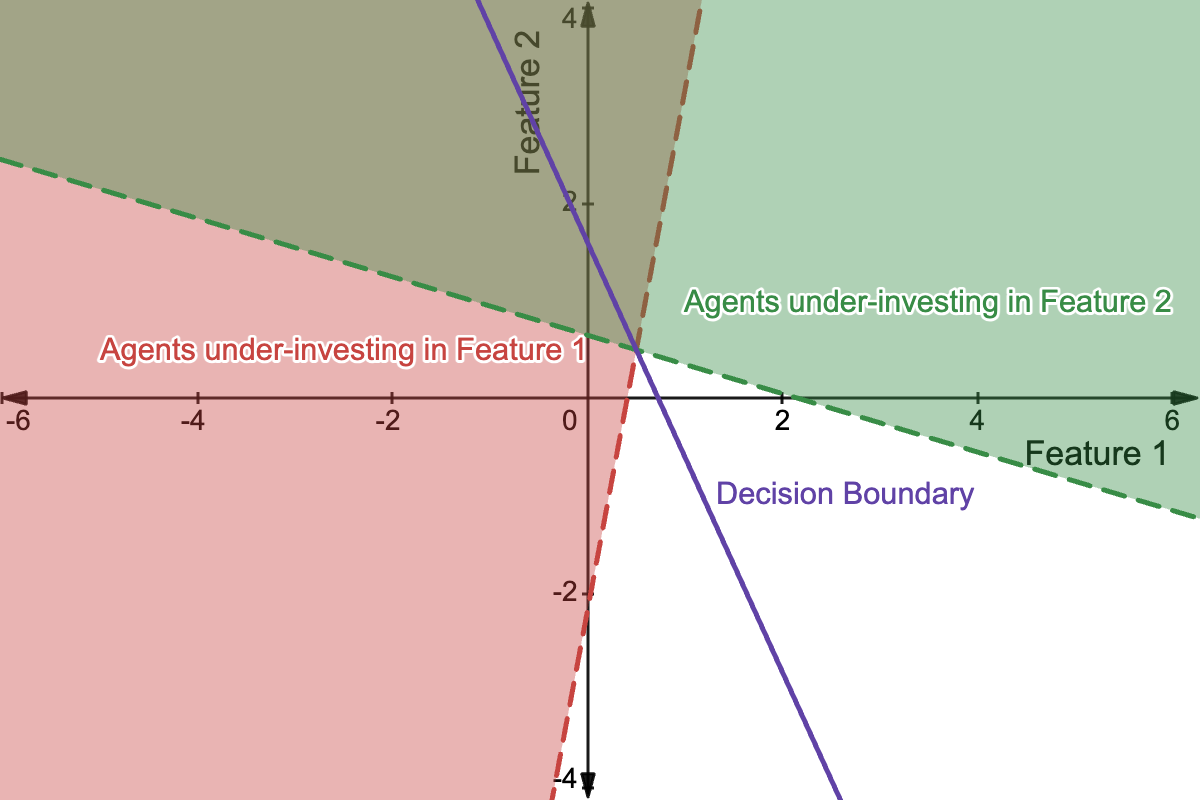
\includegraphics[width=0.5\linewidth]{Figures/desmos-graph.png}
    \caption{Caption}
    \label{fig:unde-over-invest}
\end{figure}
\end{itemize}
For instance, for $\gamma = 0.5$, $\norm{\vtheta}_2=\norm{\vw(\vtheta)}_2$ occurs when $w(\theta) = 0.5425$ and $\theta = 0.6880$ for $w(\theta)<\theta$. Therefore, for $\theta_0 = 0.5$, \eqref{eq:example_underinvest_1} and \eqref{eq:example_underinvest_2} will divide the feature space as in Figure~\ref{fig:unde-over-invest}. 
 
As seen in Figure~\ref{fig:unde-over-invest}, agents with high Feature 2 and low Feature 1 will under-invest in Feature 1 and 2. These agents will not make it to the decision boundary because of under-investment. On the other hand, the agents in the white space of Figure~\ref{fig:unde-over-invest} will over-invest in both features and pass the decision boundary. Their utility will be lower than the non-biased case since they have a higher cost due to aiming for a perceived decision boundary, but they will pass it. 
 
Compared to the non-strategic case, the firm will suffer additional loss only because of agents that over-invest. Therefore, the firm only needs to minimize the loss for agents that manipulate their features and over-invest in both features. It is necessary to note that the discussion above only tells us which agents will under-invest or over-invest in either feature and does not tell us which agents will or will not qualify. For the budgeted problem, the statements remain valid. However, not all the agents will manipulate their features, and only a subset of agents will. 


\section{Details of Numerical Experiments}\label{sec:app-numerical-details}
\paragraph{Details for Example~\ref{ex:firm-benefit-hurt} and Figure~\ref{fig:firm-benefit-hurt-dist}}For the scenario where the firm is negatively affected by the biased response is Example~\ref{ex:firm-benefit-hurt} we used $\vmu_1^T=(2, 4)$ and $\vmu_0^T=(2, 3)$ with $\Sigma_1=\begin{psmallmatrix}0.5 & 0 \\ 0 & 0.5 \end{psmallmatrix}$ and $\Sigma_0=\begin{psmallmatrix}1 & 0.5 \\ 0.5 & 1 \end{psmallmatrix}$, and we multiplied the generated data by 10. For the scenario where the firm benefits from agents' biased response we let $\vmu_1^T=(3, 5)$ and let the rest of the parameters be the same as the first scenario, i.e., $\vmu_0^T=(2, 3)$ with $\Sigma_1=\begin{psmallmatrix}0.5 & 0 \\ 0 & 0.5 \end{psmallmatrix}$ and $\Sigma_0=\begin{psmallmatrix}1 & 0.5 \\ 0.5 & 1 \end{psmallmatrix}$, and we multiplied the generated data by 10. In both scenarios, we let $B=5$. 

We used the Prelec function described in Section~\ref{sec:model} for the behavioral response. Solving the optimization problem takes a considerable amount of time for a large number of data points, here $20,000$, so we used the equivalent of the optimization problem for agents' movement and dictated the movement straight to each data point instead of solving the optimization.

To model agents' behavioral responses, we first identified the agents that would attempt to manipulate their features. Then, we used the movement function with the specified mode, either ``B'' or ``NB'', to move the data points and create a new dataset for post-response. 

For the last row of Figure~\ref{fig:firm-benefit-hurt-dist} we used $\vmu_1^T=(4, 4)$ and $\vmu_0^T=(2, 3)$ with $\Sigma_1=\begin{psmallmatrix}1 & 0 \\ 0 & 1 \end{psmallmatrix}$ and $\Sigma_0=\begin{psmallmatrix}3 & 0 \\ 0 & 1 \end{psmallmatrix}$, and we multiplied the generated data by 10. We used $B=10$.

\paragraph{Details for Figure~\ref{fig:BR-illustration}, Figure~\ref{fig:BR-illustration-quad-cost}, and Figure~\ref{fig:BR-illustration-lin-cost}} We generated 150 data points using different distributions for each feature. Feature 1 was sampled from $\mathcal{N}(700, 200)-\mathcal{D}((0, 20, 50, 100),(0.6, 0.2, 0.1, 0.1))$ where the second term is a discrete distribution selecting 0 with $p=0.6$, 20 with $p=0.2$, 50 with $0.1$, and 100 with $p=0.1$. Feature 2 was sampled from $1500-\Gamma(4, 100)$. We used a $Score$ column to label each individual for later. The score was calculated from the feature weights $(0.65, 0.35)$. We then used a sigmoid function to assign approval probability and label the sampled data points: $\frac{1}{1+\exp(-0.8\times (\frac{x}{10}-80))}$. We assigned the labels using the calculated approval probability and a random number generator. After generating the dataset, we used two copies, one for behavioral response and one for non-behavioral response. 

In Figure~\ref{fig:BR-illustration}, for agents' response to the algorithm, we calculated the agents that can afford the response with a budget of $B=100$ and performed an optimization problem on only those agents. We solved a cost minimization problem for each agent in the band specified by Lemma~\ref{lemma:band-optimization}: $\argmin_\vx cost=\norm{\vx-\vx_0}_2$ s.t. $\vtheta^T\vx\ge\theta_0$. For the behavioral case, we used $\gamma=0.5$, and the optimization problem $\argmin_\vx cost=\norm{\vx-\vx_0}_2$ s.t. $\vw(\vtheta)^T\vx\ge\theta_0$. 

In Figure~\ref{fig:BR-illustration-quad-cost}, for agents' response to the algorithm, we calculated the agents that can afford the response with a budget of $B=100$ and performed an optimization problem on only those agents. We solved a cost minimization problem for each agent in the band specified by Lemma~\ref{lemma:quad-cost-band}: $\argmin_\vx cost=\sum_i c_i(x_i-x_{0, i})^2$ s.t. $\vtheta^T\vx\ge\theta_0$. For the behavioral case, we used $\gamma=0.5$, and the optimization problem $\argmin_\vx cost=\sum_i c_i(x_i-x_{0, i})^2$ s.t. $\vw(\vtheta)^T\vx\ge\theta_0$. 

In Figure~\ref{fig:BR-illustration-lin-cost}, for agents' response to the algorithm, we calculated the agents that can afford the response with a budget of $B=100$ and performed an optimization problem on only those agents. We solved a cost minimization problem for each agent in the band specified by Lemma~\ref{lemma:manhattan-cost-band}: $\argmin_\vx cost=\vc^T|\vx-\vx_0|$ s.t. $\vtheta^T\vx\ge\theta_0$. For the behavioral case, we used $\gamma=0.5$, and the optimization problem $\argmin_\vx cost=\vc^T|\vx-\vx_0|$ s.t. $\vw(\vtheta)^T\vx\ge\theta_0$. 
%\section{Agents' Welfare}\label{app:welfare}
Figure~\ref{fig:SW-regions} highlights the change in utility when agents are behaviorally biased (vs. when they were rational) across different regions in the feature space, with the regions generated based on the firm's optimal choice of threshold and agents' responses to it. In particular, the utility of agents in the green-highlighted region (this is $\sY(\vtheta_\text{B}, \theta_{0,\text{B}}) \cap \sN(\vtheta_\text{NB}, \theta_{0,\text{NB}})$ in Proposition~\ref{prop:mismatch-actual-b}) increases when they are behaviorally biased. One subset of agents in this region are those 
%$\sY(\vtheta_\text{B}, \theta_{0,\text{B}}) \cap \sN(\vtheta_\text{NB}, \theta_{0,\text{NB}})\cap \sA(\vtheta_\text{NB}, \theta_{0, \text{NB}})$ where 
who in the rational case exert effort to get admitted and have a utility $r-c(\vx,\vx_0)$, whereas in the behaviorally biased case they attain utility $r > r-c(\vx,\vx_0)$ as they get admitted without any effort (and they correctly assume so). Another one is %subset is $(\sY(\vtheta_\text{B}, \theta_{0,\text{B}}) \cap \sN(\vtheta_\text{NB}, \theta_{0,\text{NB}}))/\sA(\vtheta_\text{NB}, \theta_{0,\text{NB}})$ which is 
the subset of agents who would not try to get to the decision boundary in the rational case (and so have utility of $0$), but in the behavioral case, they are receiving utility $r$ without any movement and due to the change of the decision boundary. For the numerical example in the bottom row of Figure~\ref{fig:firm-benefit-hurt-dist}, there are more agents in this green-highlighted region than in the remaining red-highlighted regions (where biased agents have lower utility than rational agents), leading to an overall higher welfare for all agents when they are biased compared to when they were rational. 

\begin{figure}[ht]
    \centering
    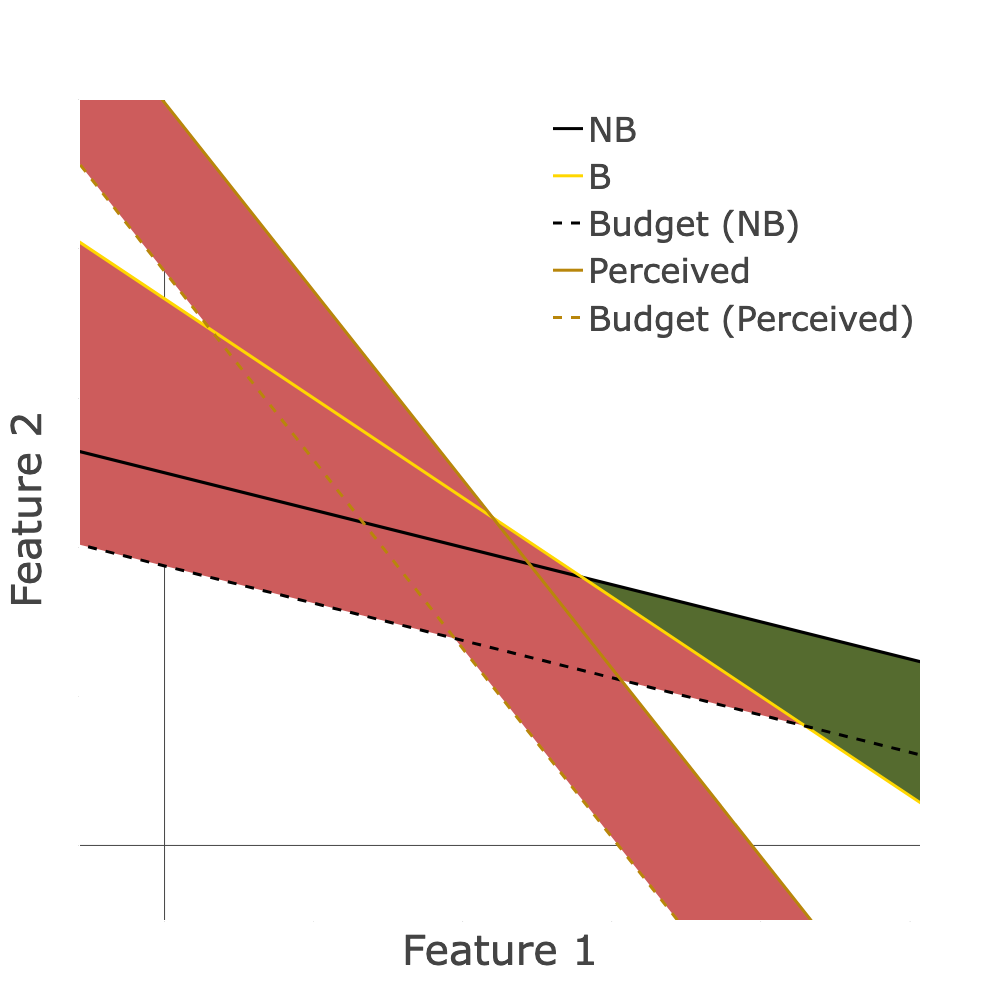
\includegraphics[width=0.4\linewidth]{Figures/SW_highlighted regions.png}
    \caption{Regions where agents have higher (green) or lower (red) utility when biased vs. when rational.}
    \Description[Welfare regions]{Regions where agents have higher (green) or lower (red) utility when biased vs. when rational.}
    \label{fig:SW-regions}
\end{figure}
\section{Piece-wise Cost Function Solution}\label{sec:app-piece-wise-sol}
Consider a setting similar to the piece-wise cost function described. To decide the feature to spend $B_1$ of the budget, we are comparing $\frac{c_1}{\theta_1}$, $\frac{c_1}{\theta_2}$, and $\frac{c_1}{\theta_3}$ as they all have the same cost for the first step of the budget. Without loss of generality imagine we have $\frac{c_1}{\theta_1} < \frac{c_1}{\theta_2} < \frac{c_1}{\theta_3}$, therefore, we choose to allocate the $B_1$ amount of our budget to the first feature. For $B_2$, we do a similar comparison but we have to use $c_2$ for the first feature since the first feature is now in the second step, i.e., we compare $\frac{c_2}{\theta_1}$, $\frac{c_1}{\theta_2}$, and $\frac{c_1}{\theta_3}$. This could lead to resulting in investing in another feature, for example, if we have $\frac{c_1}{\theta_2} < \frac{c_2}{\theta_1} < \frac{c_1}{\theta_3}$, we would choose the second feature and invest $B_2$ in that feature. We continue this reasoning until we have reached the boundary. We designed our user study so the participants did not need to calculate if they reached the decision boundary and had all participants spend all their budgets. 

As seen in Figure~\ref{fig:2d-approx-illustration}, the quadratic cost movement differs from norm-2 movement, which moves the point to the closest point on the decision boundary. The piece-wise function we use for our user study is similar to a quadratic cost function with $c_2=0.85c_1$ and a decision boundary $0.78x_1+0.22x_2=70$ for the two-dimensional case. 

% \section{User Study Questions}
% \clearpage
\section{Survey Questionnaire}\label{sec:app-survey}

This appendix contains the full text of the survey used in this study. The scenarios were assigned randomly. 

\subsection{Scenario 1 - Familiar}
Your friend is applying for a job and needs help. The company they are applying to uses an AI (Artificial Intelligence) tool that helps with hiring. The AI looks at two factors: the resume and the cover letter.

Right now, their score is 40 out of 100 on the resume and 60 out of 100 on the cover letter.

The company says each factor affects the final decision differently, as shown below in the graph.
\begin{figure}[ht]
    \centering
    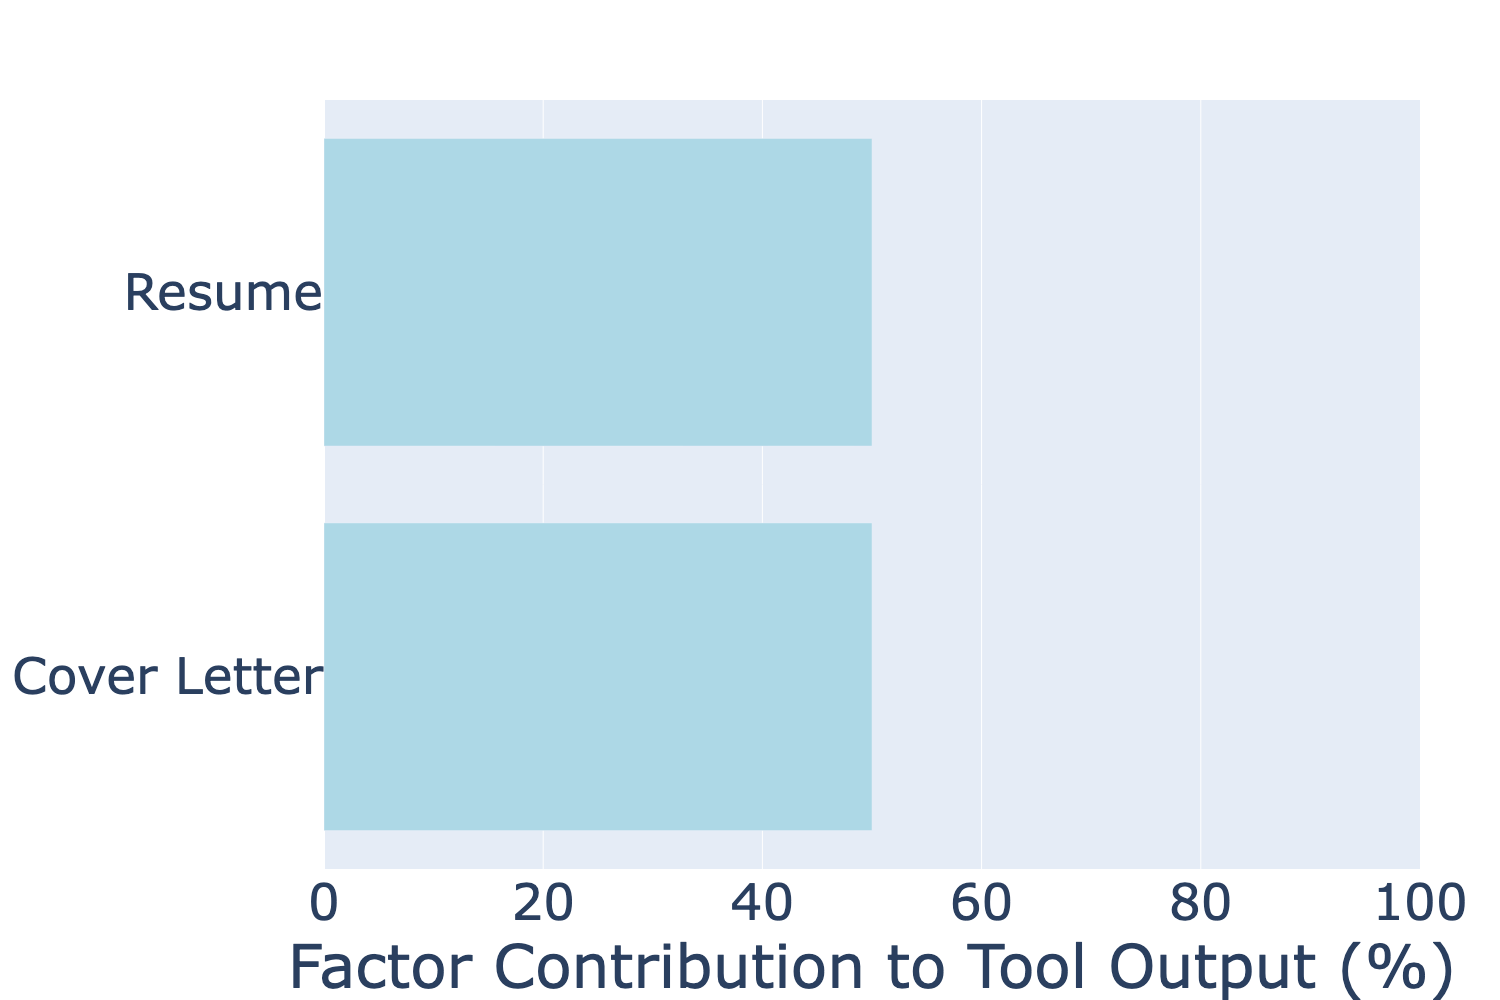
\includegraphics[width=0.4\textwidth]{Figures/2-equal.png}
    \caption{Feature weights for Scenario 1 - Familiar}
    \Description[Survey text for scenario 1 - Familiar]{The weights for scenario 1: Two features (equal)}
    \label{fig:survey-weights-scenario1}
\end{figure}

Your friend has 10 hours to get ready for the application. You want to help them decide how to use their time to improve their chances of getting a positive recommendation from the AI tool.

Your friend’s per-hour productivity rate in improving their score for each factor is as follows:
\begin{figure}[ht]
    \centering
    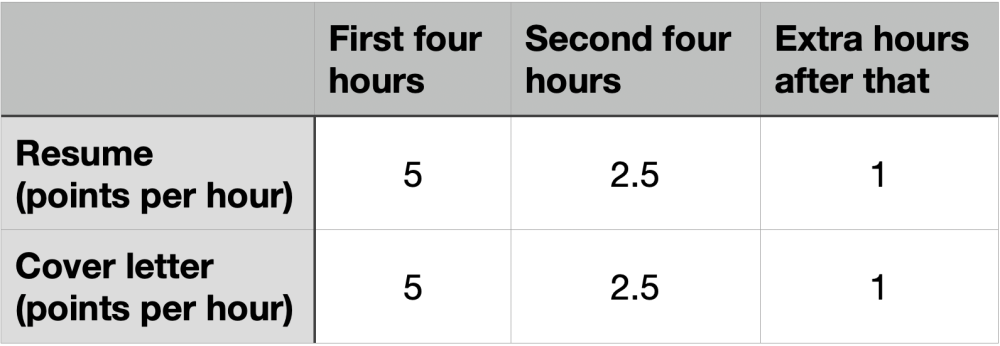
\includegraphics[width=0.5\textwidth]{Figures/cost-two.png}
    \caption{Productivity rate for Scenario 1}
    \Description[Survey text for scenario 1]{The cost description for two features}
    \label{fig:survey-cost-scenario1}
\end{figure}

The ten participants whose answers are closest to the best use of time will each receive a \$5 bonus.

\begin{itemize}
    \item Resume: \underline{\hspace{3cm}}
    \item Cover letter: \underline{\hspace{3cm}}
    \item Total: [Resume + Cover letter]
\end{itemize}


% \newpage
\subsection{Scenario 2 - Familiar}
Your friend is applying for a job and needs help. The company they are applying to uses an AI (Artificial Intelligence) tool that helps with hiring. The AI looks at two factors: the resume and the cover letter.

Right now, their score is 40 out of 100 on the resume and 60 out of 100 on the cover letter.

The company says each factor affects the final decision differently, as shown below in the graph.
\begin{figure}[ht]
    \centering
    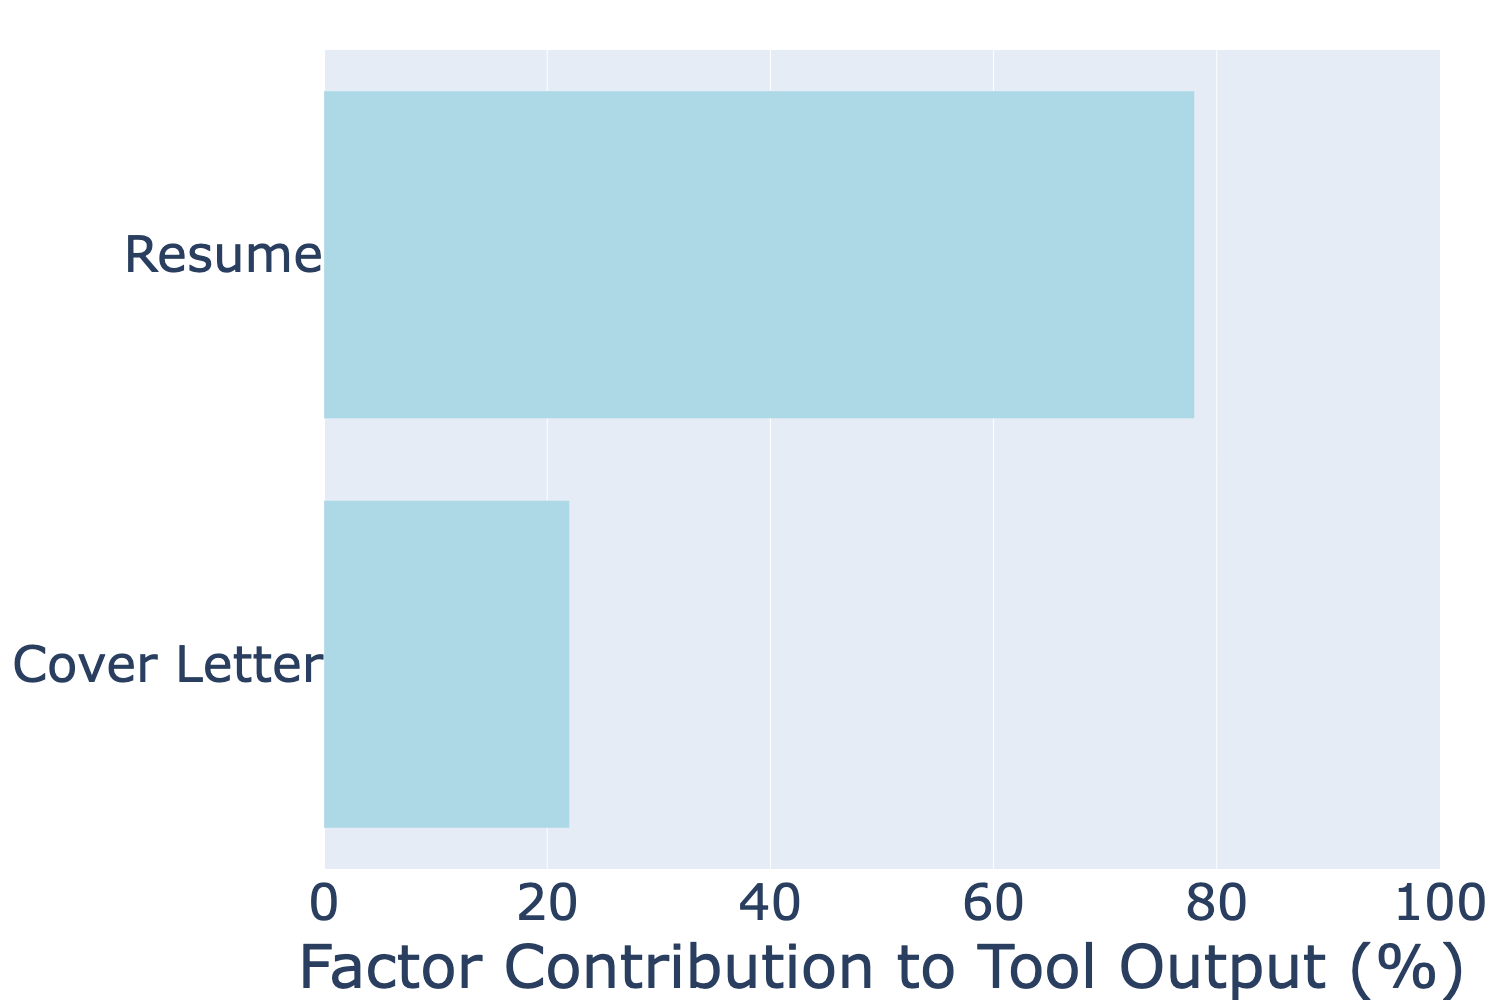
\includegraphics[width=0.4\textwidth]{Figures/2-unequal.png}
    \caption{Feature weights for Scenario 2 - Familiar}
    \Description[Survey text for scenario 2 - Familiar]{The weights for scenario 2: Two features (unequal)}
    \label{fig:survey-weights-scenario2}
\end{figure}

Your friend has 10 hours to get ready for the application. You want to help them decide how to use their time to improve their chances of getting a positive recommendation from the AI tool.

Your friend’s per-hour productivity rate in improving their score for each factor is as follows:
\begin{figure}[ht]
    \centering
    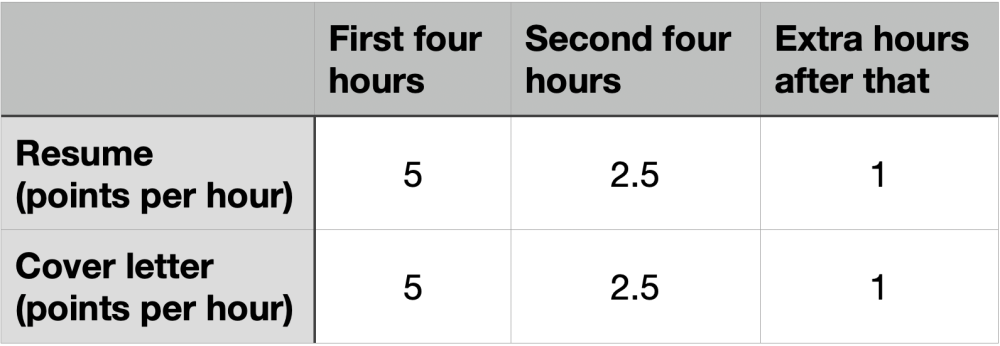
\includegraphics[width=0.5\textwidth]{Figures/cost-two.png}
    \caption{Productivity rate for Scenario 2 - Familiar}
    \Description[Survey text for scenario 2 - Familiar]{The cost description for two features}
    \label{fig:survey-cost-scenario2}
\end{figure}

The ten participants whose answers are closest to the best use of time will each receive a \$5 bonus.

\begin{itemize}
    \item Resume: \underline{\hspace{3cm}}
    \item Cover letter: \underline{\hspace{3cm}}
    \item Total: [Resume + Cover letter]
\end{itemize}


% \newpage
\subsection{Scenario 3 - Familiar}
Your friend is applying for a job and needs help. The company they are applying to uses an AI (Artificial Intelligence) tool that helps with hiring. The AI looks at four factors: the resume, the cover letter, LinkedIn profile, and on-site interview score.

Right now, their score is 60 out of 100 for on-site interview, 40 out of 100 on the resume, 60 out of 100 on the cover letter, and 65 out of 100 on the LinkedIn profile.

The company says each factor affects the final decision differently, as shown below in the graph.
\begin{figure}[ht]
    \centering
    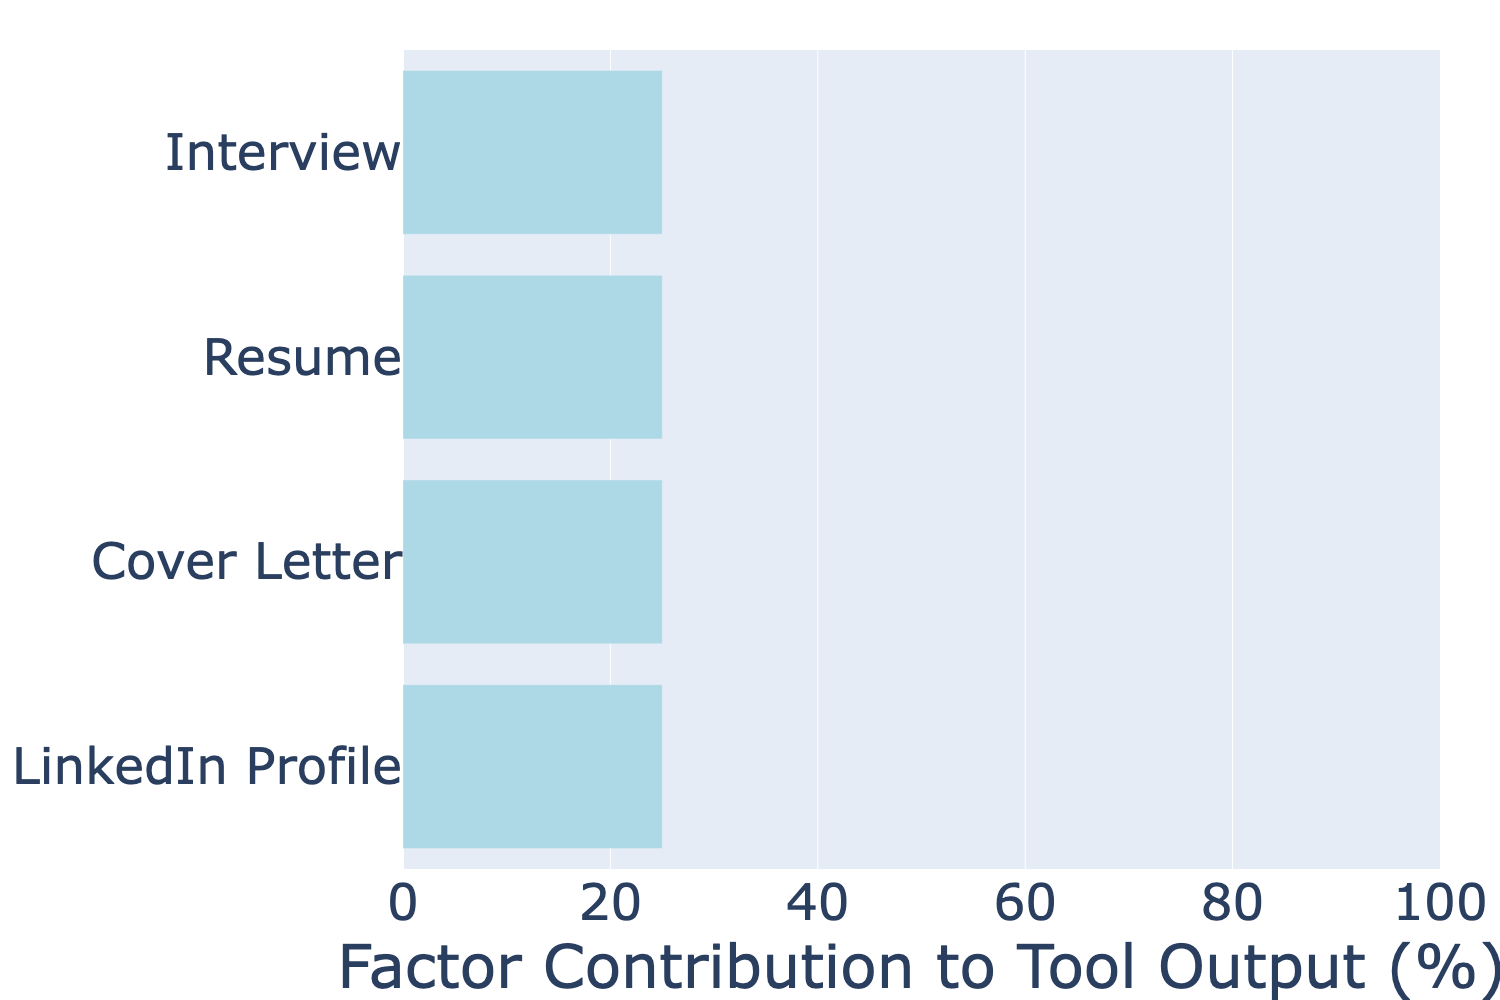
\includegraphics[width=0.4\textwidth]{Figures/4-equal.png}
    \caption{Feature weights for Scenario 3 - Familiar}
    \Description[Survey text for scenario 3 - Familiar]{The weights for scenario 3: Four features (equal)}
    \label{fig:survey-weights-scenario3}
\end{figure}

Your friend has 10 hours to get ready for the application. You want to help them decide how to use their time to improve their chances of getting a positive recommendation from the AI tool.

Your friend’s per-hour productivity rate in improving their score for each factor is as follows:
\begin{figure}[ht]
    \centering
    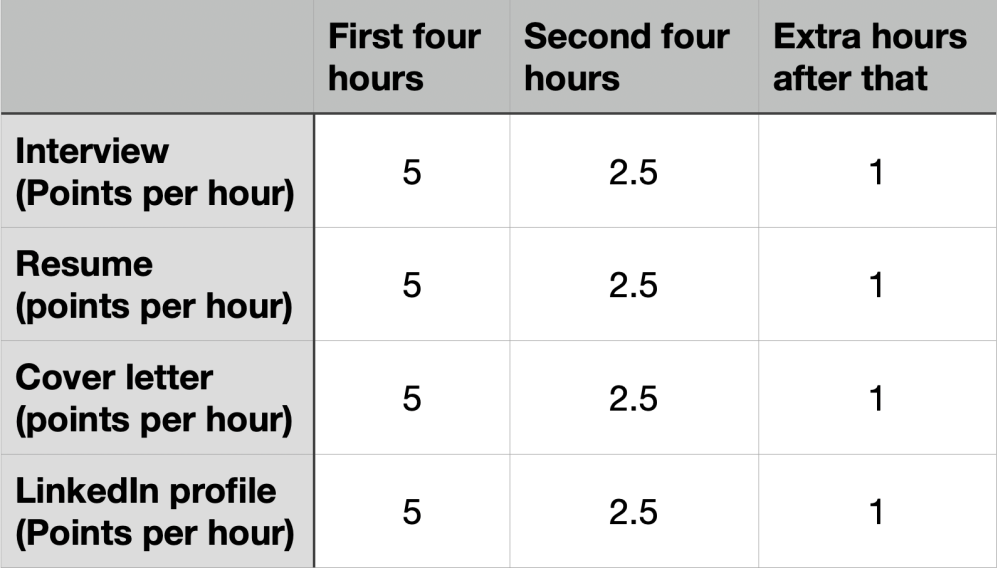
\includegraphics[width=0.4\textwidth]{Figures/cost-four.png}
    \caption{Productivity rate for Scenario 3 - Familiar}
    \Description[Survey text for scenario 3 - Familiar]{The cost description for four features}
    \label{fig:survey-cost-scenario3}
\end{figure}

The ten participants whose answers are closest to the best use of time will each receive a \$5 bonus.

\begin{itemize}
    \item Interview: \underline{\hspace{3cm}}
    \item Resume: \underline{\hspace{3cm}}
    \item Cover letter: \underline{\hspace{3cm}}
    \item LinkedIn profile: \underline{\hspace{3cm}}
    \item Total: [Interview + Resume + Cover letter + LinkedIn profile]
\end{itemize}


% \newpage
\subsection{Scenario 4 - Familiar}
Your friend is applying for a job and needs help. The company they are applying to uses an AI (Artificial Intelligence) tool that helps with hiring. The AI looks at four factors: the resume, the cover letter, LinkedIn profile, and on-site interview score.

Right now, their score is 60 out of 100 for on-site interview, 40 out of 100 on the resume, 60 out of 100 on the cover letter, and 65 out of 100 on the LinkedIn profile.

The company says each factor affects the final decision differently, as shown below in the graph.
\begin{figure}[ht]
    \centering
    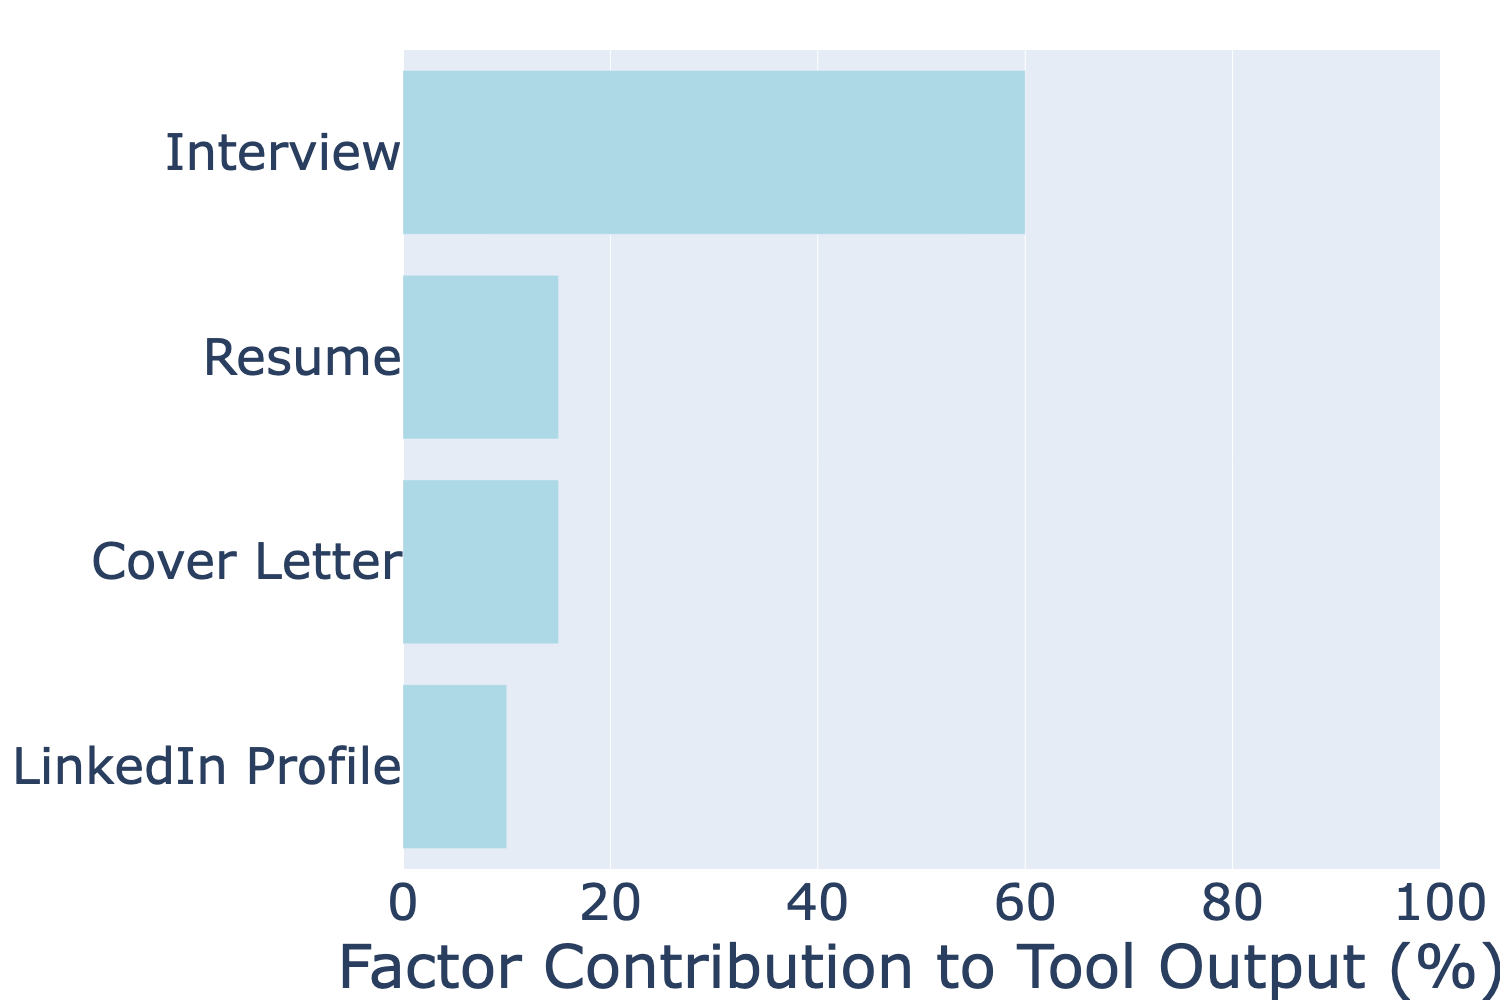
\includegraphics[width=0.4\textwidth]{Figures/4-unequal.png}
    \caption{Feature weights for Scenario 4 - Familiar}
    \Description[Survey text for scenario 4 - Familiar]{The weights for scenario 4: Four features (unequal)}
    \label{fig:survey-weights-scenario4}
\end{figure}

Your friend has 10 hours to get ready for the application. You want to help them decide how to use their time to improve their chances of getting a positive recommendation from the AI tool.

Your friend’s per-hour productivity rate in improving their score for each factor is as follows:
\begin{figure}[ht]
    \centering
    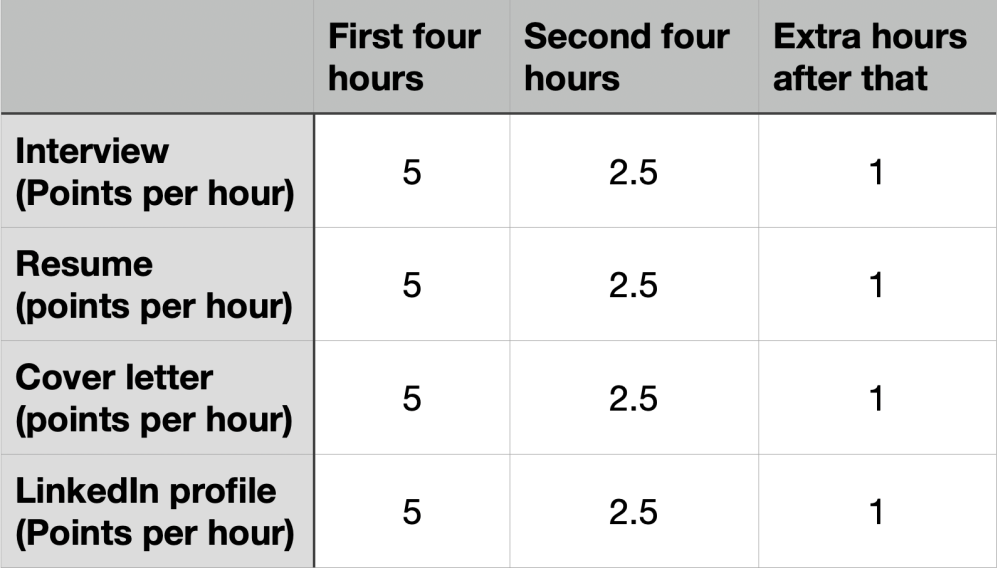
\includegraphics[width=0.4\textwidth]{Figures/cost-four.png}
    \caption{Productivity rate for Scenario 4 - Familiar}
    \Description[Survey text for scenario 4 - Familiar]{The cost description for four features}
    \label{fig:survey-cost-scenario4}
\end{figure}

The ten participants whose answers are closest to the best use of time will each receive a \$5 bonus.

\begin{itemize}
    \item Interview: \underline{\hspace{3cm}}
    \item Resume: \underline{\hspace{3cm}}
    \item Cover letter: \underline{\hspace{3cm}}
    \item LinkedIn profile: \underline{\hspace{3cm}}
    \item Total: [Interview + Resume + Cover letter + LinkedIn profile]
\end{itemize}


% \subsection{Satisfaction}
% \begin{enumerate}
%     \item The system was easy to use
%     \begin{itemize}
%         \item[ ] Extremely difficult (1)
%         \item[ ] Somewhat difficult (2)
%         \item[ ] Neither easy nor difficult (3)
%         \item[ ] Somewhat easy (4)
%         \item[ ] Extremely easy (5)
%     \end{itemize}
    
%     \item The explanation of how the tool works was useful for my goals
%     \begin{itemize}
%         \item[ ] Strongly disagree (1)
%         \item[ ] Somewhat disagree (2)
%         \item[ ] Neither agree nor disagree (3)
%         \item[ ] Somewhat agree (4)
%         \item[ ] Strongly agree (5)
%     \end{itemize}

%     \item Rate your satisfaction with the explanation
%     \begin{itemize}
%         \item[ ] Extremely dissatisfied (1)
%         \item[ ] Somewhat dissatisfied (2)
%         \item[ ] Neither satisfied nor dissatisfied (3)
%         \item[ ] Somewhat satisfied (4)
%         \item[ ] Extremely satisfied (5)
%     \end{itemize}
% \end{enumerate}

% \subsection{Understanding}
% \begin{enumerate}
%     \item I understand the explanation of how the tool works
%     \begin{itemize}
%         \item[ ] Not well at all (1)
%         \item[ ] Slightly well (2)
%         \item[ ] Moderately well (3)
%         \item[ ] Very well (4)
%         \item[ ] Extremely well (5)
%     \end{itemize}
    
%     \item How confident are you in your answer
%     \begin{itemize}
%         \item[ ] Very confident (1)
%         \item[ ] Somewhat confident (2)
%         \item[ ] Neither confident nor unsure (3)
%         \item[ ] Somewhat unsure (4)
%         \item[ ] Very unsure (5)
%     \end{itemize}

%     \item Assume the organization's tool gives the following weights: Resume (70\%) and cover letter (30\%) A person has a score of 50 out of 100 for resume and 50 out of 100 for cover letter. They spend all their time to improve their cover letter. Is this the best use of their time?
%     \begin{itemize}
%         \item[ ] Yes
%         \item[ ] No
%     \end{itemize}
% \end{enumerate}

% \subsection{Trust}
% \begin{enumerate}
%     \item Do you think that the system is trustworthy?
%     \begin{itemize}
%         \item[ ] Very safe (1)
%         \item[ ] Somewhat safe (2)
%         \item[ ] Neither safe nor unsafe (3)
%         \item[ ] Somewhat dangerous (4)
%         \item[ ] Very dangerous (5)
%     \end{itemize}
    
%     \item Is the tool efficient at what is does?
%     \begin{itemize}
%         \item[ ] Definitely not (1)
%         \item[ ] Probably not (2)
%         \item[ ] Might or might not (3)
%         \item[ ] Probably yes (4)
%         \item[ ] Definitely yes (5)
%     \end{itemize}

%     \item What is your confidence in the tool?
%     \begin{itemize}
%         \item[ ] None at all (1)
%         \item[ ] A little (2) 
%         \item[ ] A moderate amount (3)
%         \item[ ] A lot (4)
%         \item[ ] A great deal (5)
%     \end{itemize}
% \end{enumerate}

% \subsection{Task Performance}
% \begin{enumerate}
%     \item How difficult was the task?
%     \begin{itemize}
%         \item[ ] Extremely difficult (1)
%         \item[ ] Somewhat difficult (2)
%         \item[ ] Neither easy nor difficult (3)
%         \item[ ] Somewhat easy (4)
%         \item[ ] Extremely easy (5)
%     \end{itemize}
    
%     \item How successful were you at the task?
%     \begin{itemize}
%         \item[ ] Very unsuccessful (1)
%         \item[ ] Somewhat unsuccessful (2)
%         \item[ ] Neither successful not unsuccessful (3)
%         \item[ ] Somewhat successful (4)
%         \item[ ] Very successful (5)
%     \end{itemize}

%     \item How mentally demanding was the task?
%     \begin{itemize}
%         \item[ ] Very low (1)
%         \item[ ] Somewhat low (2)
%         \item[ ] Neither low nor high (3)
%         \item[ ] Somewhat high (4)
%         \item[ ] Very high (5)
%     \end{itemize}
% \end{enumerate}

% \subsection{Tech Familiarity}
% How familiar are you with the following computer and internet related items? Please don't look up anything about the terms below, as we want to know your responses based on the information you already have.
% \begin{table}[ht]
% \caption{} 
% \begin{center}
%     \begin{tabular}{llllll}
%     & \thead{Not familiar \\ at all}  & \thead{Slightly\\ familiar} & \thead{Moderately\\ familiar} & \thead{Very\\ familiar} & \thead{Extremely\\ familiar} \\
%     \hline
%     \makecell{Backpropagation} \\
%     \makecell{k-Nearest Neighbors (KNN)} \\
%     \makecell{Citrus++} \\
%     \makecell{Support Vector Machines (SVM)} \\
%     \makecell{Data Reversion} \\
%     \makecell{PyCharm} \\
%     \end{tabular}
% \end{center}
% \end{table}

% \subsection{Demographics}
% Please state your gender
% \begin{itemize}
%     \item Male
%     \item Female
%     \item Non-binary / gender non-conforming
%     \item Prefer not to say
%     \item Prefer to self-describe: \underline{\hspace{3cm}}
% \end{itemize}

% How old are you? (e.g. 19) \underline{\hspace{3cm}}

% Please state your ethnicity
% \begin{itemize}
%     \item American Indian, Alaska native
%     \item Asian
%     \item Black, African American
%     \item Hispanic, Latino, or Spanish
%     \item Middle Eastern and North African Native Hawaiian or Other Pacific Islander 
%     \item White
%     \item Prefer not to say
% \end{itemize}

% What is the highest level of education you have completed?
% \begin{itemize}
%     \item Less than a high school diploma
%     \item High school degree or equivalent (e.g. GED)
%     \item Technical, trade or vocational school AFTER high school
%     \item Some college, no degree
%     \item 2 year college (e.g. AA, AS)
%     \item 4 year college (e.g. BA, BS)
%     \item Prefer not to say
% \end{itemize}
% \newpage
\subsection{Scenario 1 - Unfamiliar}
Your friend has been diagnosed with Coronary Artery Disease (CAD) and needs to improve their health metrics to reduce the risk of a future heart attack. Their cardiologist uses an AI (Artificial Intelligence) tool to assess the likelihood of a major cardiovascular event. The AI evaluates four key health factors: LDL cholesterol (low-density lipoprotein), VO2 max (aerobic fitness), arterial stiffness index, and inflammatory markers (C-reactive protein, CRP).

Currently, their scores are as follows (higher score means healthier):
\begin{itemize}
    \item LDL Cholesterol: 60 out of 100
    \item VO2 Max: 40 out of 100
    \item Arterial Stiffness Index: 60 out of 100
    \item Inflammatory Markers: 65 out of 100
\end{itemize}

Each factor has a different weight in the AI’s calculation, as shown in the graph below. Some factors are more critical than others for reducing overall risk.
\begin{figure}[ht]
    \centering
    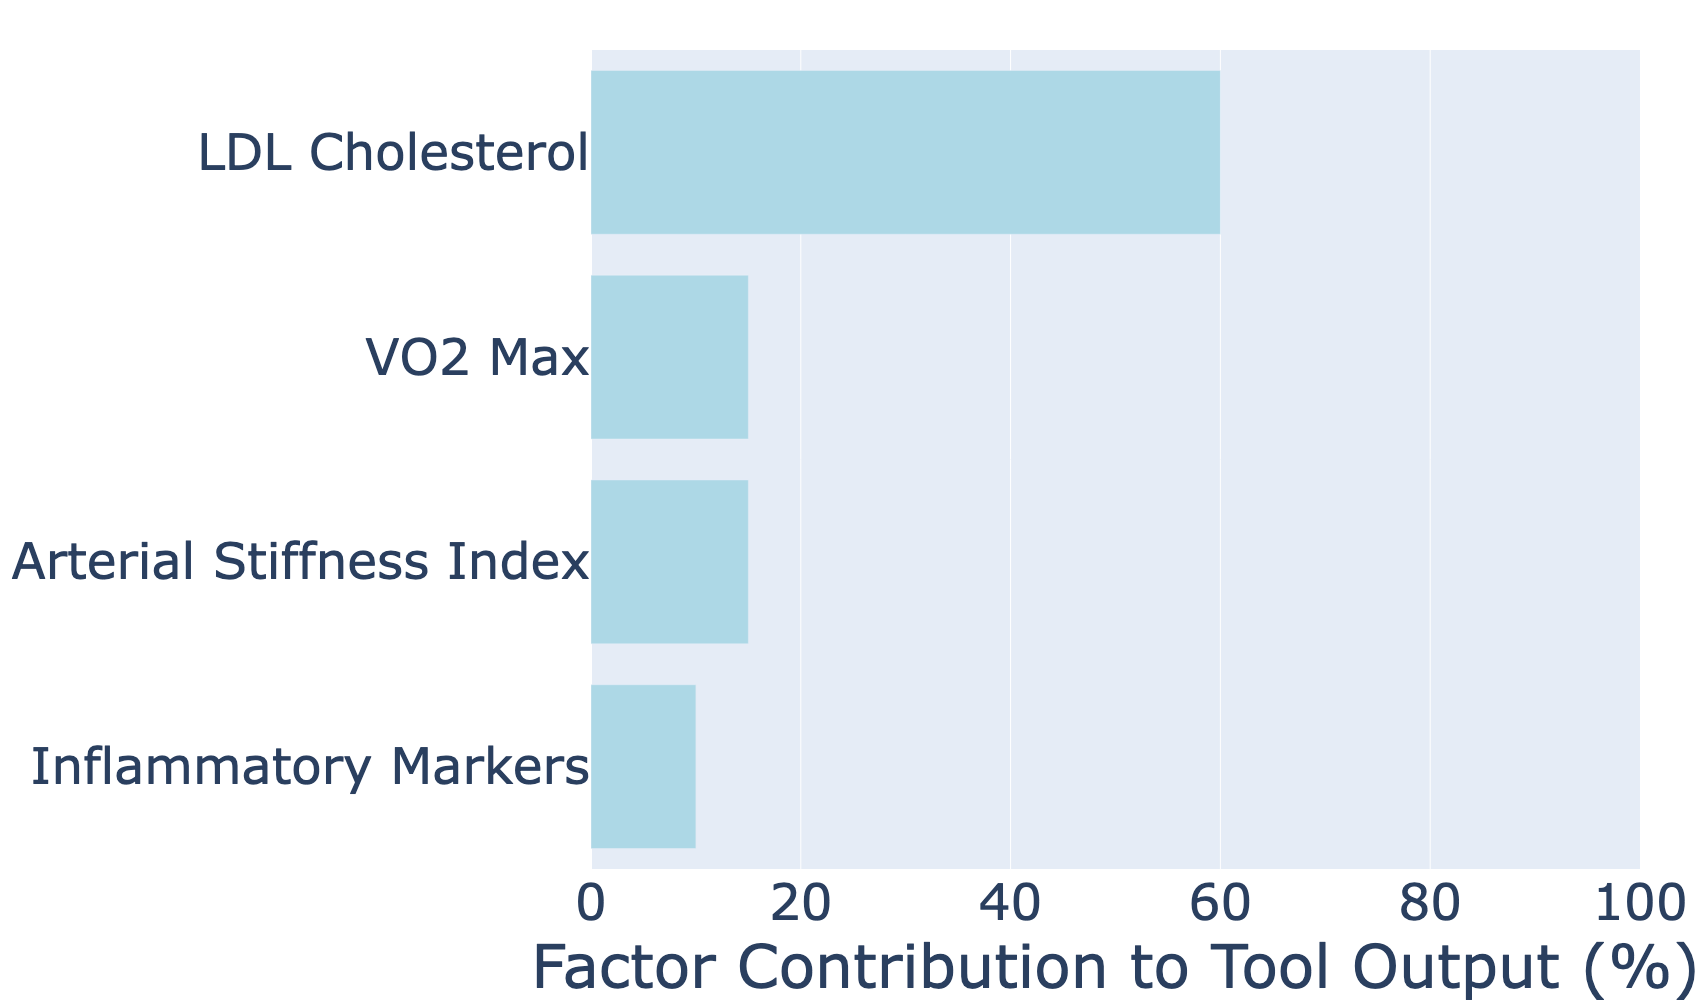
\includegraphics[width=0.4\textwidth]{Figures/4_unf_unbal.png}
    \caption{Feature weights for Scenario 1 - Unfamiliar}
    \Description[Survey text for scenario 1 - Unfamiliar]{The weights for scenario 1: 4 features (unequal)}
    \label{fig:survey-weights-scenario1-unf}
\end{figure}

Your friend has 10 weeks to improve these scores before their next check-up. You want to help them decide how to allocate their time and efforts to reduce their risk of a cardiovascular event.

Your friend’s per-hour productivity rate in improving their score for each factor is as follows:

\begin{figure}[ht]
    \centering
    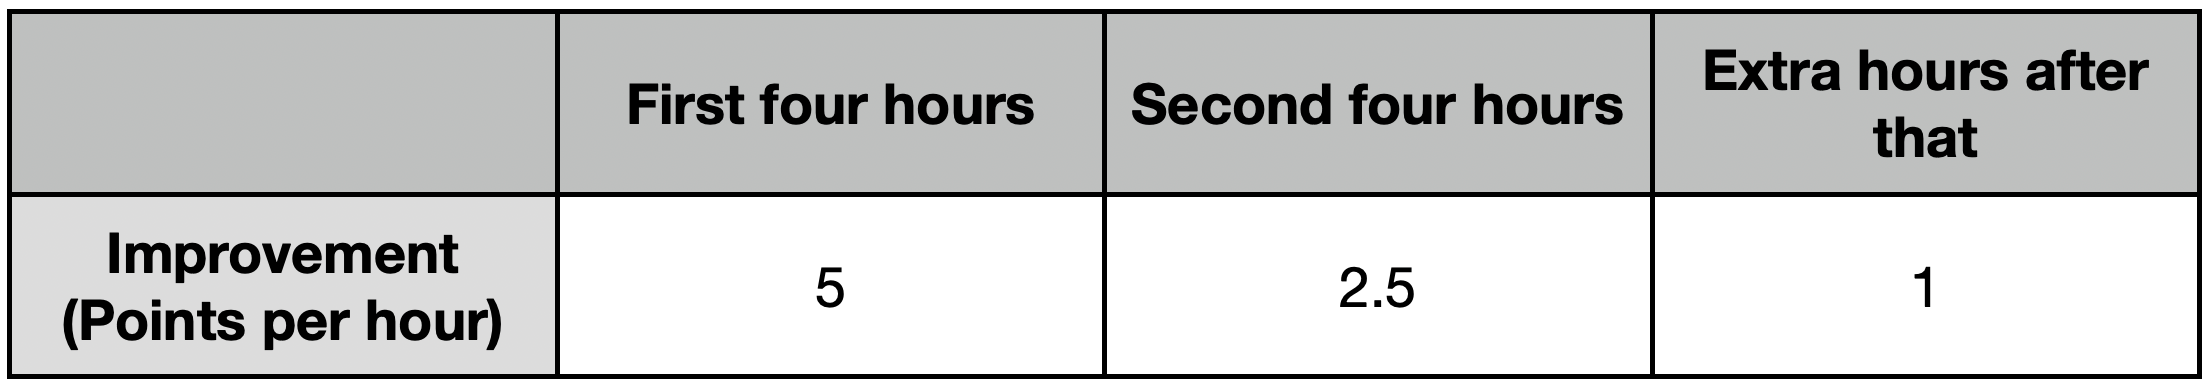
\includegraphics[width=0.5\textwidth]{Figures/rate-unf.png}
    \caption{Productivity rate for Scenario 1 - Unfamiliar}
    \Description[Survey text for scenario 1 - Unfamiliar]{The cost description}
    \label{fig:survey-cost-scenario1-unf}
\end{figure}

Based on this, how should your friend use their 10 weeks improving the factors to maximize their chances of a healthy outcome?

The ten participants whose answers are closest to the best use of time will each receive a \$5 bonus. 

\begin{itemize}
    \item LDL cholesterol (diet): \underline{\hspace{2cm}}
    \item VO2 max (exercise): \underline{\hspace{2cm}}
    \item Arterial Stiffness Index (yoga and medications): \underline{\hspace{2cm}}
    \item Inflammatory Markers (stress and sleep): \underline{\hspace{2cm}}
    \item Total: [VO2 max + LDL cholesterol + Arterial Stiffness Index + Inflammatory Markers]
\end{itemize}

% \newpage
\subsection{Scenario 2 - Unfamiliar}
Your friend has been diagnosed with Coronary Artery Disease (CAD) and needs to improve their health metrics to reduce the risk of a future heart attack. Their cardiologist uses an AI (Artificial Intelligence) tool to assess the likelihood of a major cardiovascular event. The AI evaluates four key health factors: LDL cholesterol (low-density lipoprotein), VO2 max (aerobic fitness), arterial stiffness index, and inflammatory markers (C-reactive protein, CRP).

Currently, their scores are as follows (higher score means healthier):
\begin{itemize}
    \item LDL Cholesterol: 60 out of 100
    \item VO2 Max: 40 out of 100
    \item Arterial Stiffness Index: 60 out of 100
    \item Inflammatory Markers: 65 out of 100
\end{itemize}

Each factor has a different weight in the AI’s calculation, as shown in the graph below. Some factors are more critical than others for reducing overall risk.
\begin{figure}[ht]
    \centering
    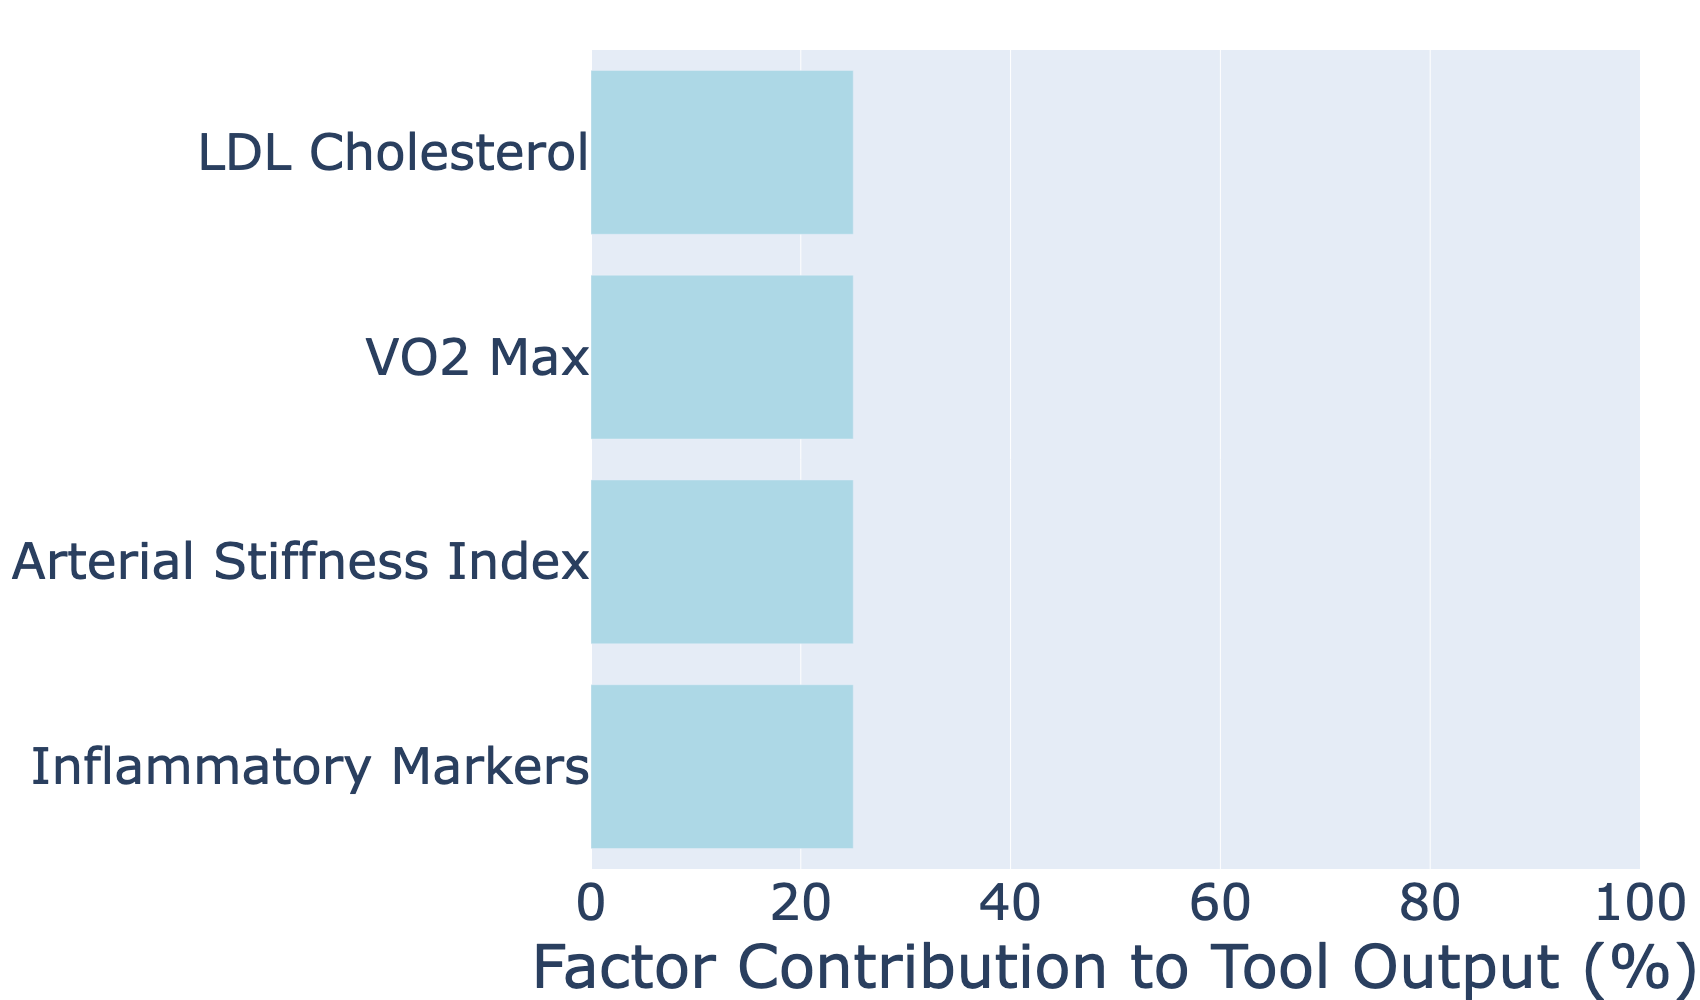
\includegraphics[width=0.4\textwidth]{Figures/4_unf_bal.png}
    \caption{Feature weights for Scenario 2 - Unfamiliar}
    \Description[Survey text for scenario 2 - Unfamiliar]{The weights for scenario 1: 4 features (equal)}
    \label{fig:survey-weights-scenario2-unf}
\end{figure}

Your friend has 10 weeks to improve these scores before their next check-up. You want to help them decide how to allocate their time and efforts to reduce their risk of a cardiovascular event.

Your friend’s per-hour productivity rate in improving their score for each factor is as follows:

\begin{figure}[ht]
    \centering
    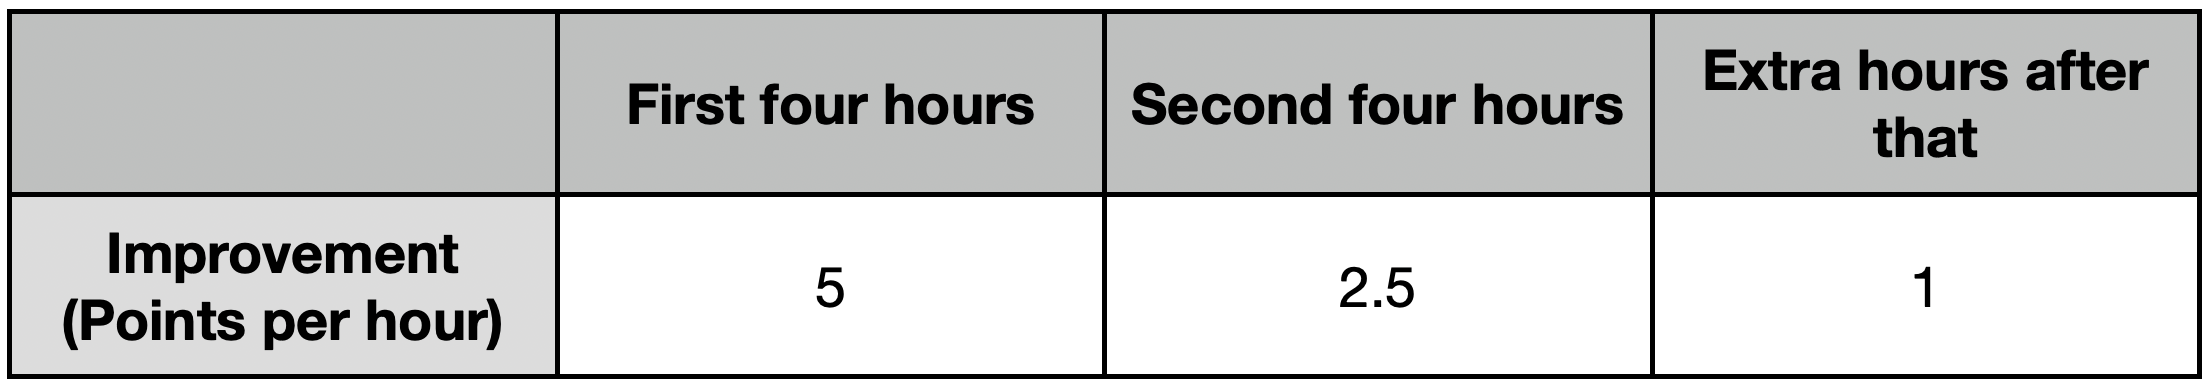
\includegraphics[width=0.5\textwidth]{Figures/rate-unf.png}
    \caption{Productivity rate for Scenario 2 - Unfamiliar}
    \Description[Survey text for scenario 2 - Unfamiliar]{The cost description}
    \label{fig:survey-cost-scenario2-unf}
\end{figure}

Based on this, how should your friend use their 10 weeks improving the factors to maximize their chances of a healthy outcome?

The ten participants whose answers are closest to the best use of time will each receive a \$5 bonus. 

\begin{itemize}
    \item LDL cholesterol (diet): \underline{\hspace{2cm}}
    \item VO2 max (exercise): \underline{\hspace{2cm}}
    \item Arterial Stiffness Index (yoga and medications): \underline{\hspace{2cm}}
    \item Inflammatory Markers (stress and sleep): \underline{\hspace{2cm}}
    \item Total: [VO2 max + LDL cholesterol + Arterial Stiffness Index + Inflammatory Markers]
\end{itemize}

% \newpage
\subsection{Scenario 3 - Unfamiliar}
Your friend has been diagnosed with Coronary Artery Disease (CAD) and needs to improve their health metrics to reduce the risk of a future heart attack. Their cardiologist uses an AI (Artificial Intelligence) tool to assess the likelihood of a major cardiovascular event. The AI evaluates two key health factors: LDL cholesterol (low-density lipoprotein) and VO2 max (aerobic fitness).

Currently, their scores are as follows (higher score means healthier):
\begin{itemize}
    \item LDL Cholesterol: 60 out of 100
    \item VO2 Max: 40 out of 100
\end{itemize}

Each factor has a different weight in the AI’s calculation, as shown in the graph below. Some factors are more critical than others for reducing overall risk.
\begin{figure}[ht]
    \centering
    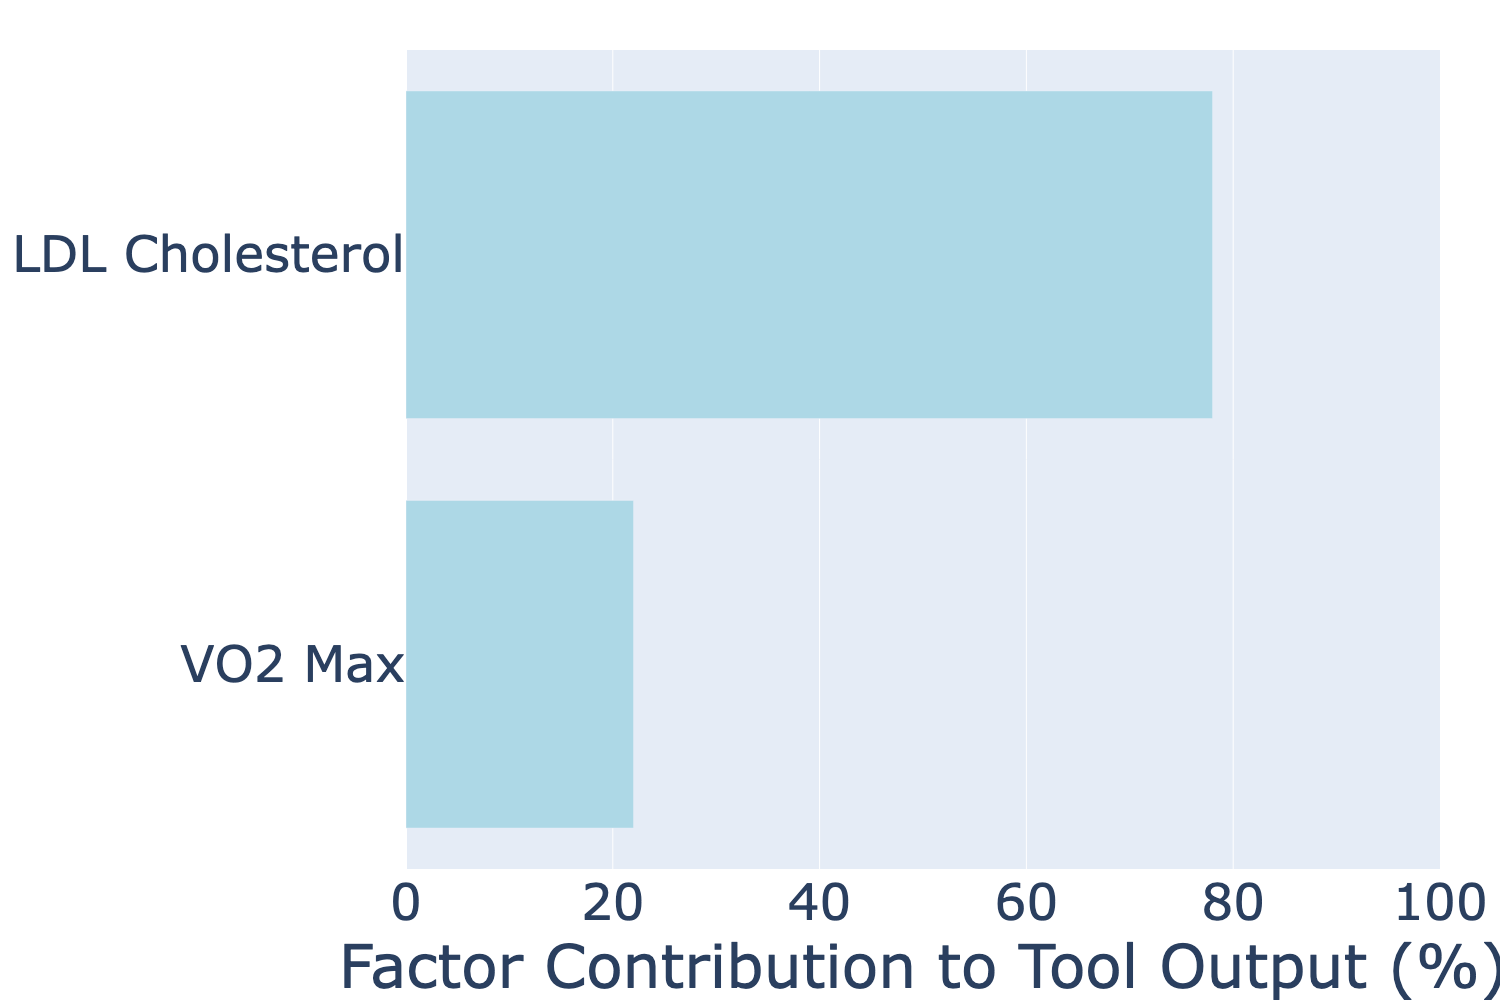
\includegraphics[width=0.4\textwidth]{Figures/2_unf_unbal.png}
    \caption{Feature weights for Scenario 3 - Unfamiliar}
    \Description[Survey text for scenario 3 - Unfamiliar]{The weights for scenario 1: 2 features (unequal)}
    \label{fig:survey-weights-scenario3-unf}
\end{figure}

Your friend has 10 weeks to improve these scores before their next check-up. You want to help them decide how to allocate their time and efforts to reduce their risk of a cardiovascular event.

Your friend’s per-hour productivity rate in improving their score for each factor is as follows:

\begin{figure}[ht]
    \centering
    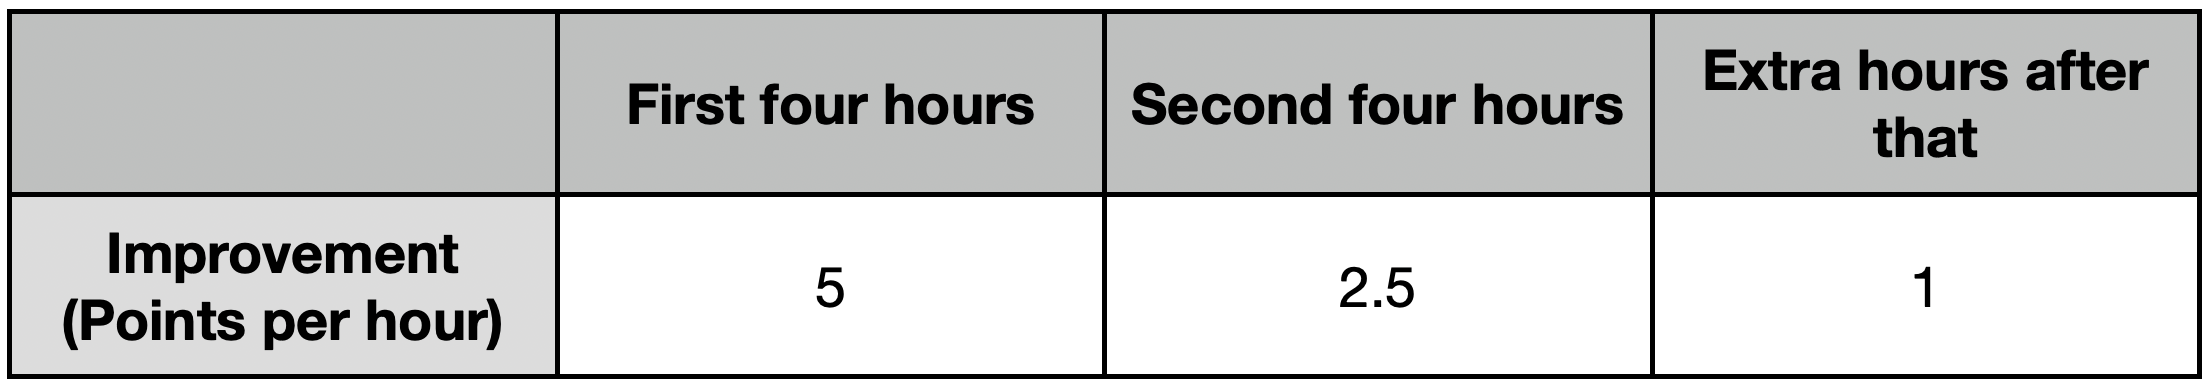
\includegraphics[width=0.4\textwidth]{Figures/rate-unf.png}
    \caption{Productivity rate for Scenario 3 - Unfamiliar}
    \Description[Survey text for scenario 3 - Unfamiliar]{The cost description}
    \label{fig:survey-cost-scenario3-unf}
\end{figure}

Based on this, how should your friend use their 10 weeks improving the factors to maximize their chances of a healthy outcome?

The ten participants whose answers are closest to the best use of time will each receive a \$5 bonus. 

\begin{itemize}
    \item LDL cholesterol (diet): \underline{\hspace{3cm}}
    \item VO2 max (exercise): \underline{\hspace{3cm}}
    \item Total: [VO2 max + LDL cholesterol]
\end{itemize}

% \newpage
\subsection{Scenario 4 - Unfamiliar}
Your friend has been diagnosed with Coronary Artery Disease (CAD) and needs to improve their health metrics to reduce the risk of a future heart attack. Their cardiologist uses an AI (Artificial Intelligence) tool to assess the likelihood of a major cardiovascular event. The AI evaluates two key health factors: LDL cholesterol (low-density lipoprotein) and VO2 max (aerobic fitness).

Currently, their scores are as follows (higher score means healthier):
\begin{itemize}
    \item LDL Cholesterol: 60 out of 100
    \item VO2 Max: 40 out of 100
\end{itemize}

Each factor has a different weight in the AI’s calculation, as shown in the graph below. Some factors are more critical than others for reducing overall risk.
\begin{figure}[ht]
    \centering
    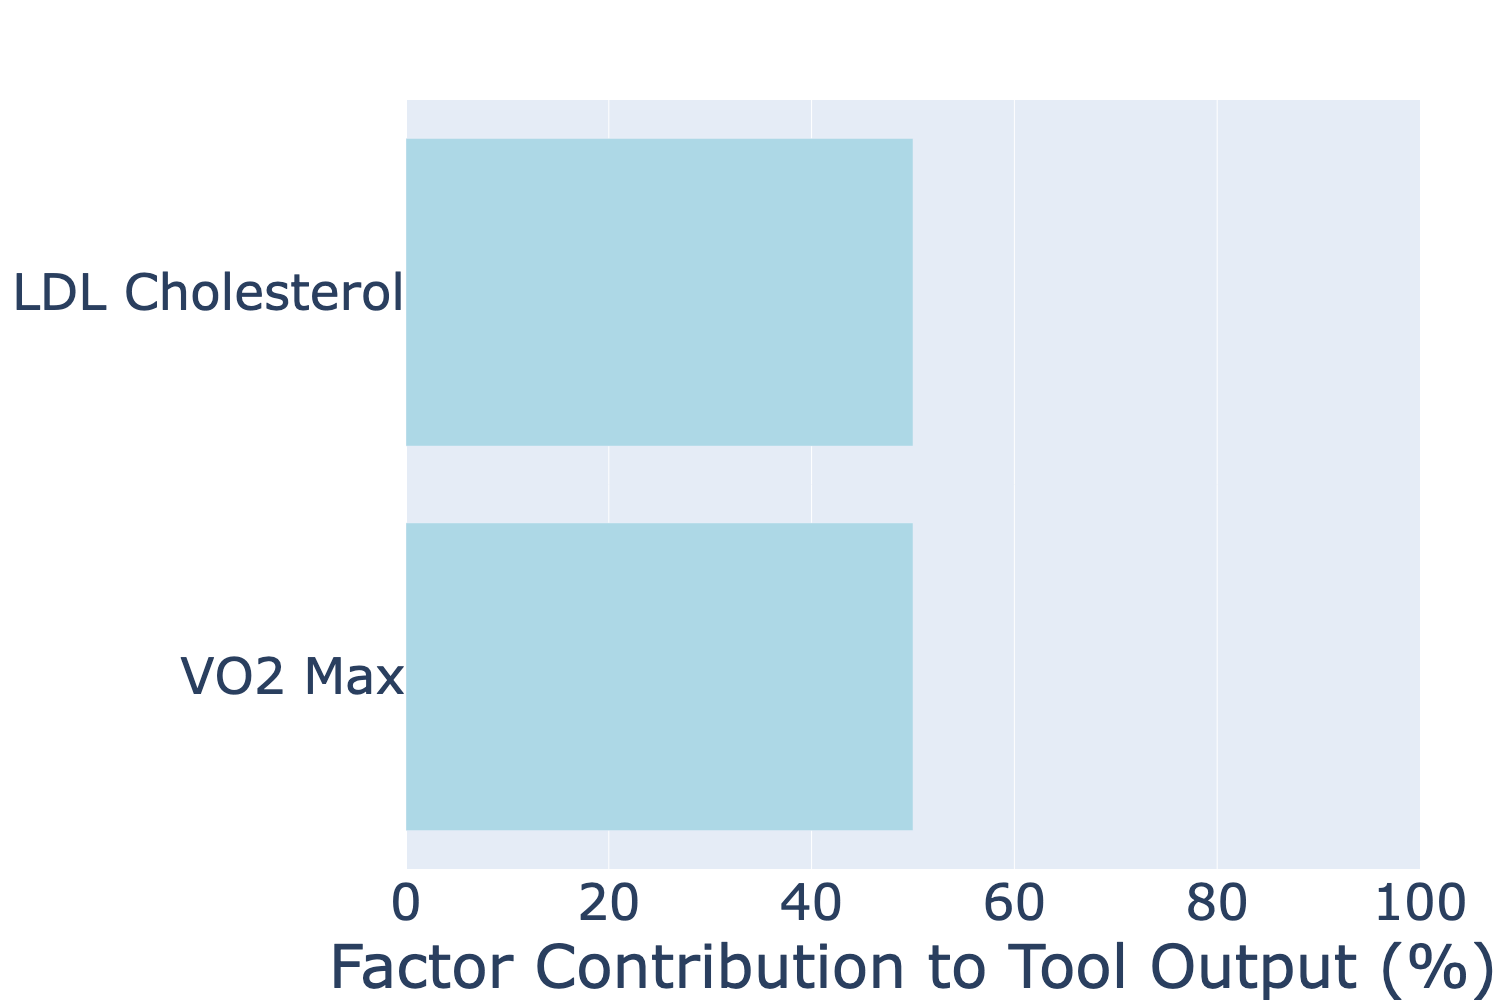
\includegraphics[width=0.4\textwidth]{Figures/2_unf_bal.png}
    \caption{Feature weights for Scenario 4 - Unfamiliar}
    \Description[Survey text for scenario 4 - Unfamiliar]{The weights for scenario 1: 2 features (equal)}
    \label{fig:survey-weights-scenario4-unf}
\end{figure}

Your friend has 10 weeks to improve these scores before their next check-up. You want to help them decide how to allocate their time and efforts to reduce their risk of a cardiovascular event.

Your friend’s per-hour productivity rate in improving their score for each factor is as follows:

\begin{figure}[ht]
    \centering
    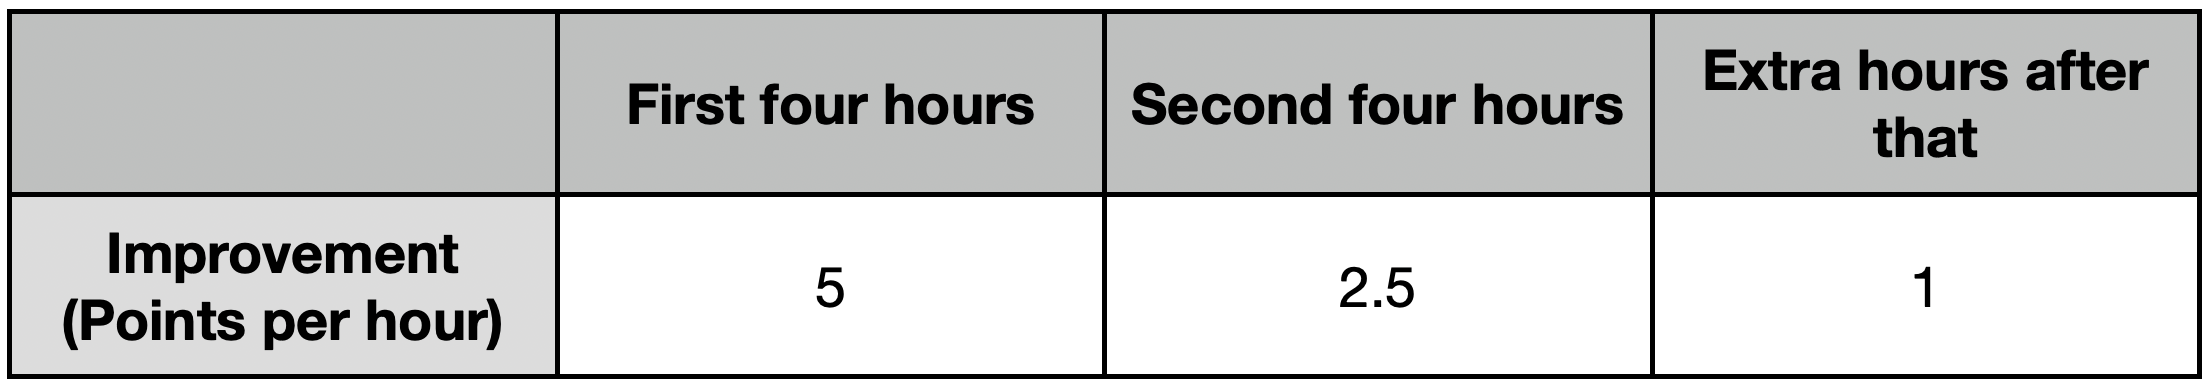
\includegraphics[width=0.5\textwidth]{Figures/rate-unf.png}
    \caption{Productivity rate for Scenario 4 - Unfamiliar}
    \Description[Survey text for scenario 4 - Unfamiliar]{The cost description}
    \label{fig:survey-cost-scenario4-unf}
\end{figure}

Based on this, how should your friend use their 10 weeks improving the factors to maximize their chances of a healthy outcome?

The ten participants whose answers are closest to the best use of time will each receive a \$5 bonus. 

\begin{itemize}
    \item LDL cholesterol (diet): \underline{\hspace{3cm}}
    \item VO2 max (exercise): \underline{\hspace{3cm}}
    \item Total: [VO2 max + LDL cholesterol]
\end{itemize}
{% \clearpage
\section{Statistical Analysis of The User Study}\label{sec:app-stats-survey}
% In this section we provide statistical details and analysis of the user study results. To begin with, we use Kullback-Leibler (KL) Divergence to compare the distributions of multi-dimensional responses between the different conditions. This allows us to measure how different the response distributions are without flattening them. The results of the KL divergence analysis is as follows:
% \begin{itemize}
%     \item There is a noticeable divergence between the distributions of balanced and unbalanced scenarios for 2-features in the familiar context (KL Divergence: 1400.53)
%     \item The KL divergence between the distributions of balanced and unbalanced scenarios for 2-features in the unfamiliar context is higher than the familiar context (KL Divergence: 2344.15). 
%     \item There is a noticeable divergence between the distributions of balanced and unbalanced scenarios for 4-features in the familiar context (KL Divergence: 324596.76)
%     \item There is a noticeable divergence between the distributions of balanced and unbalanced scenarios for 4-features in the unfamiliar context (KL Divergence: 762145.96)
% \end{itemize}


% This tells us that the distribution of balanced and unbalanced scenarios are different in all of the scenarios. The KL divergence for 4-feature scenarios are much higher than the KL divergence for 2-feature scenarios suggesting that the impact of having unbalanced features when we have more features is higher. That said, the large KL divergence for 4-feature scenarios can be a result of dimensionality. This can because in higher-dimensional spaces, distributions have more ways to differ from each other, leading to greater dissimilarity. As the number of dimensions increases, the volume of space increases exponentially, and distributions in higher dimensions tend to become more sparse, making it more likely that the two distributions differ in areas of the space.

% In Figure~\ref{fig:ks-test} we visualized the differences in investments in the most important feature using their distributions. We compare the distributions of balanced an unbalanced cases and we use the same feature for balanced scenarios (first feature in all the scenarios). The KS statistics in Table~\ref{table:KS-stats} tells us that there is a significant difference in the investment in the most important feature between balanced and unbalanced cases when the context is unfamiliar. 

% \begin{figure}[ht]
%     \centering
%     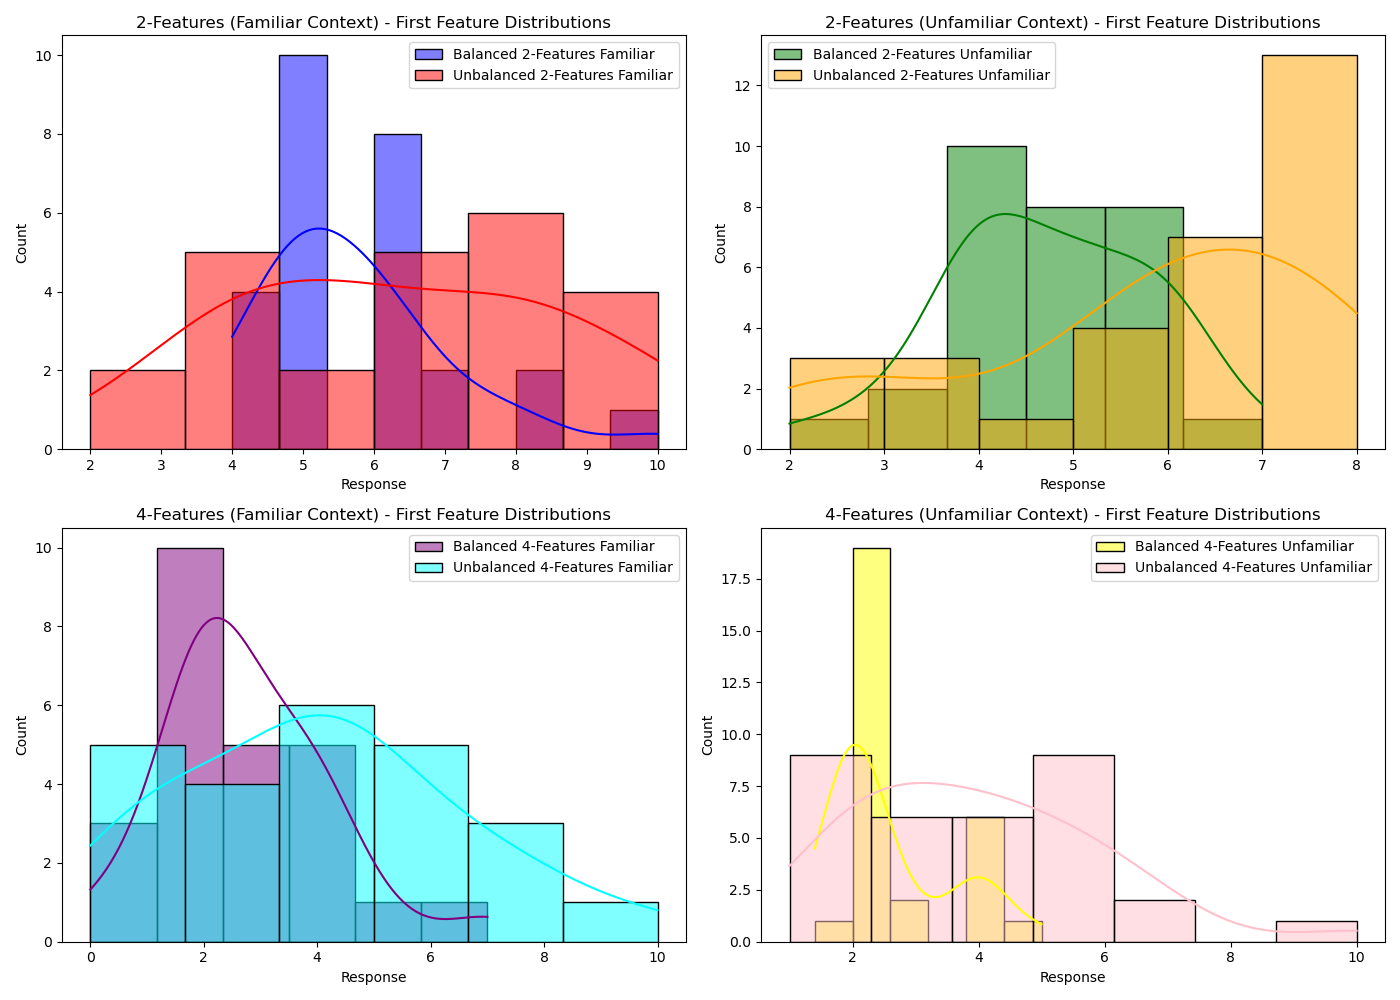
\includegraphics[width=0.7\linewidth]{Figures/ks_test_distributions.png}
%     \caption{Comparison of the distributions of the investments in the most important feature in balanced and unbalanced scenarios for 2-feature and 4-feature tasks in familiar and unfamiliar contexts.}
%     \Description[distribution comparisons]{Comparison of the distributions of balanced and unbalanced scenarios for 2-feature and 4-feature tasks in familiar and unfamiliar contexts.}
%     \label{fig:ks-test}
% \end{figure}

% \begin{table}[ht]
%     \caption{KS test statistics}\label{table:KS-stats}
%     \begin{center}
%         \begin{tabular}{lll}
%          &\textbf{KS statistic} &\textbf{P-value} \\
%         \hline \\[-4.8pt]
%         2-features (Familiar) & 0.31 & 0.15 \\
%         2-features (Unfamiliar) & 0.39 & 0.01 \\
%         4-features (Familiar) & 0.34 & 0.09 \\
%         4-features (Unfamiliar) & 0.45 & 0.002
%         \end{tabular}
%     \end{center}
% \end{table}
\begin{table*}[t]
    \caption{Mean and variance statistics}\label{table:mv-stats}
    \begin{center}
        \begin{tabular}{lllll}
         & Feature 1 ($\mu$, $\sigma^2$) & Feature 2 ($\mu$, $\sigma^2$) & Feature 3 ($\mu$, $\sigma^2$) & Feature 4 ($\mu$, $\sigma^2$)\\
        \hline \\[-4.8pt]
        2-features balanced (Familiar) & (5.74, 1.87) & (4.26, 1.87) & -- & -- \\
        2-features unbalanced (Familiar) & (6.31, 5.39) & (3.69, 5.39) & -- & -- \\
        4-features balanced (Familiar) & (2.76, 2.11) & (4.32, 3.64) & (1.68, 0.73) & (1.24, 0.77) \\
        4-features unbalanced (Familiar) & (4.06, 6.35) & (2.52, 1.81) & (1.73, 0.98) & (1.69, 2.34) \\
        2-features balanced (Unfamiliar) & (4.73, 1.25) & (5.27, 1.25) & -- & -- \\
        2-features unbalanced (Unfamiliar) & (5.74, 3.65) & (4.26, 3.65) & -- & -- \\
        4-features balanced (Unfamiliar) & (2.59, 0.90) & (3.43, 1.57) & (2.04, 0.33) & (1.94, 0.96) \\
        4-features unbalanced (Unfamiliar) & (3.97, 3.97) & (2.59, 1.21) & (1.72, 0.70) & (1.72, 1.85) 
        \end{tabular}
    \end{center}
\end{table*}

The mean and variance for investments in each scenario can be seen in Table~\ref{table:mv-stats}. As we can see the variance for unfamiliar cases are generally lower than the familiar cases. We can also see the increase in mean of the most important feature as we go from balanced cases to unbalanced cases. 

Comparing balanced and unbalanced cases, we can see higher variances in unbalanced cases. In both 2-feature and 4-feature unbalanced scenarios, we generally see a higher variance for at least one feature (often the ``most important'' feature). For Instance, in 2-features (Familiar), the variance jumps from 1.87 (balanced) to 5.39 (unbalanced) for each feature, indicating participants were much less consistent about how they allocated time when features were unbalanced. We also see greater mean differences in unbalanced cases. In unbalanced scenarios, the gap between the means of the ``most important'' and ``least important'' features tends to be larger. For example, 2-features (Familiar) goes from (5.74 vs. 4.26) in balanced (a 1.48 difference) to (6.31 vs. 3.69) in unbalanced (a 2.62 difference). 
If we compare the cases based on the number of features, we see more concentrated investments. In 2-feature scenarios, participants often put higher average investment (e.g., 5–6 hours) into the more important feature, with moderate variance. For four features, we see lower means per feature but spread out. With four features, each feature's mean is lower because participants are splitting the same total budget (10 hours) across more options. We still see unbalanced vs. balanced patterns: In 4-features balanced (Familiar), the second feature has the highest mean (4.32) but also a fairly high variance (3.64). In 4-features unbalanced (Familiar), Feature 1 jumps to a higher mean (4.06) with a large variance (6.35), suggesting participants differ widely on how much to allocate to that top feature.
}


\vfill

% \end{document}





\end{document}
\endinput
%%
%% End of file `sample-manuscript.tex'.
